% Options for packages loaded elsewhere
\PassOptionsToPackage{unicode}{hyperref}
\PassOptionsToPackage{hyphens}{url}
\documentclass[
]{article}
\usepackage{xcolor}
\usepackage[margin=1in]{geometry}
\usepackage{amsmath,amssymb}
\setcounter{secnumdepth}{-\maxdimen} % remove section numbering
\usepackage{iftex}
\ifPDFTeX
  \usepackage[T1]{fontenc}
  \usepackage[utf8]{inputenc}
  \usepackage{textcomp} % provide euro and other symbols
\else % if luatex or xetex
  \usepackage{unicode-math} % this also loads fontspec
  \defaultfontfeatures{Scale=MatchLowercase}
  \defaultfontfeatures[\rmfamily]{Ligatures=TeX,Scale=1}
\fi
\usepackage{lmodern}
\ifPDFTeX\else
  % xetex/luatex font selection
\fi
% Use upquote if available, for straight quotes in verbatim environments
\IfFileExists{upquote.sty}{\usepackage{upquote}}{}
\IfFileExists{microtype.sty}{% use microtype if available
  \usepackage[]{microtype}
  \UseMicrotypeSet[protrusion]{basicmath} % disable protrusion for tt fonts
}{}
\makeatletter
\@ifundefined{KOMAClassName}{% if non-KOMA class
  \IfFileExists{parskip.sty}{%
    \usepackage{parskip}
  }{% else
    \setlength{\parindent}{0pt}
    \setlength{\parskip}{6pt plus 2pt minus 1pt}}
}{% if KOMA class
  \KOMAoptions{parskip=half}}
\makeatother
\usepackage{color}
\usepackage{fancyvrb}
\newcommand{\VerbBar}{|}
\newcommand{\VERB}{\Verb[commandchars=\\\{\}]}
\DefineVerbatimEnvironment{Highlighting}{Verbatim}{commandchars=\\\{\}}
% Add ',fontsize=\small' for more characters per line
\usepackage{framed}
\definecolor{shadecolor}{RGB}{248,248,248}
\newenvironment{Shaded}{\begin{snugshade}}{\end{snugshade}}
\newcommand{\AlertTok}[1]{\textcolor[rgb]{0.94,0.16,0.16}{#1}}
\newcommand{\AnnotationTok}[1]{\textcolor[rgb]{0.56,0.35,0.01}{\textbf{\textit{#1}}}}
\newcommand{\AttributeTok}[1]{\textcolor[rgb]{0.13,0.29,0.53}{#1}}
\newcommand{\BaseNTok}[1]{\textcolor[rgb]{0.00,0.00,0.81}{#1}}
\newcommand{\BuiltInTok}[1]{#1}
\newcommand{\CharTok}[1]{\textcolor[rgb]{0.31,0.60,0.02}{#1}}
\newcommand{\CommentTok}[1]{\textcolor[rgb]{0.56,0.35,0.01}{\textit{#1}}}
\newcommand{\CommentVarTok}[1]{\textcolor[rgb]{0.56,0.35,0.01}{\textbf{\textit{#1}}}}
\newcommand{\ConstantTok}[1]{\textcolor[rgb]{0.56,0.35,0.01}{#1}}
\newcommand{\ControlFlowTok}[1]{\textcolor[rgb]{0.13,0.29,0.53}{\textbf{#1}}}
\newcommand{\DataTypeTok}[1]{\textcolor[rgb]{0.13,0.29,0.53}{#1}}
\newcommand{\DecValTok}[1]{\textcolor[rgb]{0.00,0.00,0.81}{#1}}
\newcommand{\DocumentationTok}[1]{\textcolor[rgb]{0.56,0.35,0.01}{\textbf{\textit{#1}}}}
\newcommand{\ErrorTok}[1]{\textcolor[rgb]{0.64,0.00,0.00}{\textbf{#1}}}
\newcommand{\ExtensionTok}[1]{#1}
\newcommand{\FloatTok}[1]{\textcolor[rgb]{0.00,0.00,0.81}{#1}}
\newcommand{\FunctionTok}[1]{\textcolor[rgb]{0.13,0.29,0.53}{\textbf{#1}}}
\newcommand{\ImportTok}[1]{#1}
\newcommand{\InformationTok}[1]{\textcolor[rgb]{0.56,0.35,0.01}{\textbf{\textit{#1}}}}
\newcommand{\KeywordTok}[1]{\textcolor[rgb]{0.13,0.29,0.53}{\textbf{#1}}}
\newcommand{\NormalTok}[1]{#1}
\newcommand{\OperatorTok}[1]{\textcolor[rgb]{0.81,0.36,0.00}{\textbf{#1}}}
\newcommand{\OtherTok}[1]{\textcolor[rgb]{0.56,0.35,0.01}{#1}}
\newcommand{\PreprocessorTok}[1]{\textcolor[rgb]{0.56,0.35,0.01}{\textit{#1}}}
\newcommand{\RegionMarkerTok}[1]{#1}
\newcommand{\SpecialCharTok}[1]{\textcolor[rgb]{0.81,0.36,0.00}{\textbf{#1}}}
\newcommand{\SpecialStringTok}[1]{\textcolor[rgb]{0.31,0.60,0.02}{#1}}
\newcommand{\StringTok}[1]{\textcolor[rgb]{0.31,0.60,0.02}{#1}}
\newcommand{\VariableTok}[1]{\textcolor[rgb]{0.00,0.00,0.00}{#1}}
\newcommand{\VerbatimStringTok}[1]{\textcolor[rgb]{0.31,0.60,0.02}{#1}}
\newcommand{\WarningTok}[1]{\textcolor[rgb]{0.56,0.35,0.01}{\textbf{\textit{#1}}}}
\usepackage{graphicx}
\makeatletter
\newsavebox\pandoc@box
\newcommand*\pandocbounded[1]{% scales image to fit in text height/width
  \sbox\pandoc@box{#1}%
  \Gscale@div\@tempa{\textheight}{\dimexpr\ht\pandoc@box+\dp\pandoc@box\relax}%
  \Gscale@div\@tempb{\linewidth}{\wd\pandoc@box}%
  \ifdim\@tempb\p@<\@tempa\p@\let\@tempa\@tempb\fi% select the smaller of both
  \ifdim\@tempa\p@<\p@\scalebox{\@tempa}{\usebox\pandoc@box}%
  \else\usebox{\pandoc@box}%
  \fi%
}
% Set default figure placement to htbp
\def\fps@figure{htbp}
\makeatother
\setlength{\emergencystretch}{3em} % prevent overfull lines
\providecommand{\tightlist}{%
  \setlength{\itemsep}{0pt}\setlength{\parskip}{0pt}}
\usepackage{bookmark}
\IfFileExists{xurl.sty}{\usepackage{xurl}}{} % add URL line breaks if available
\urlstyle{same}
\hypersetup{
  hidelinks,
  pdfcreator={LaTeX via pandoc}}

\author{}
\date{\vspace{-2.5em}}

\begin{document}

\section{Package Downloads}\label{package-downloads}

\begin{Shaded}
\begin{Highlighting}[]
\CommentTok{\# Run this chunk top{-}to{-}bottom in a fresh R session to ensure all required}
\CommentTok{\# packages are available. It safely skips anything already installed.}

\NormalTok{cran\_repo }\OtherTok{\textless{}{-}} \StringTok{"https://cloud.r{-}project.org"}
\FunctionTok{options}\NormalTok{(}\AttributeTok{repos =} \FunctionTok{c}\NormalTok{(}\AttributeTok{CRAN =}\NormalTok{ cran\_repo))}

\ControlFlowTok{if}\NormalTok{ (}\SpecialCharTok{!}\FunctionTok{requireNamespace}\NormalTok{(}\StringTok{"BiocManager"}\NormalTok{, }\AttributeTok{quietly =} \ConstantTok{TRUE}\NormalTok{)) \{}
  \FunctionTok{install.packages}\NormalTok{(}\StringTok{"BiocManager"}\NormalTok{, }\AttributeTok{repos =}\NormalTok{ cran\_repo)}
\NormalTok{\}}

\NormalTok{BiocManager}\SpecialCharTok{::}\FunctionTok{install}\NormalTok{(}\AttributeTok{version =} \StringTok{"3.21"}\NormalTok{, }\AttributeTok{ask =} \ConstantTok{FALSE}\NormalTok{, }\AttributeTok{update =} \ConstantTok{FALSE}\NormalTok{)}

\NormalTok{install\_if\_missing }\OtherTok{\textless{}{-}} \ControlFlowTok{function}\NormalTok{(pkgs, installer) \{}
\NormalTok{  missing\_pkgs }\OtherTok{\textless{}{-}}\NormalTok{ pkgs[}\SpecialCharTok{!}\FunctionTok{vapply}\NormalTok{(pkgs, requireNamespace,}
                               \AttributeTok{FUN.VALUE =} \FunctionTok{logical}\NormalTok{(}\DecValTok{1}\NormalTok{), }\AttributeTok{quietly =} \ConstantTok{TRUE}\NormalTok{)]}
  \ControlFlowTok{if}\NormalTok{ (}\FunctionTok{length}\NormalTok{(missing\_pkgs) }\SpecialCharTok{\textgreater{}} \DecValTok{0}\NormalTok{) \{}
    \FunctionTok{installer}\NormalTok{(missing\_pkgs)}
\NormalTok{  \}}
  \FunctionTok{invisible}\NormalTok{(}\ConstantTok{NULL}\NormalTok{)}
\NormalTok{\}}

\FunctionTok{install\_if\_missing}\NormalTok{(}
  \AttributeTok{pkgs =} \FunctionTok{c}\NormalTok{(}\StringTok{"devtools"}\NormalTok{, }\StringTok{"GenomeInfoDb"}\NormalTok{, }\StringTok{"tidyverse"}\NormalTok{),}
  \AttributeTok{installer =} \ControlFlowTok{function}\NormalTok{(pkgs) }\FunctionTok{install.packages}\NormalTok{(pkgs, }\AttributeTok{repos =}\NormalTok{ cran\_repo)}
\NormalTok{)}

\FunctionTok{install\_if\_missing}\NormalTok{(}
  \AttributeTok{pkgs =} \FunctionTok{c}\NormalTok{(}\StringTok{"DESeq2"}\NormalTok{, }\StringTok{"org.Hs.eg.db"}\NormalTok{),}
  \AttributeTok{installer =} \ControlFlowTok{function}\NormalTok{(pkgs) BiocManager}\SpecialCharTok{::}\FunctionTok{install}\NormalTok{(pkgs, }\AttributeTok{ask =} \ConstantTok{FALSE}\NormalTok{, }\AttributeTok{update =} \ConstantTok{FALSE}\NormalTok{)}
\NormalTok{)}
\end{Highlighting}
\end{Shaded}

\section{Section 1}\label{section-1}

\subsection{Section 1a}\label{section-1a}

\begin{Shaded}
\begin{Highlighting}[]
\CommentTok{\# Attach the library}
\FunctionTok{library}\NormalTok{(org.Hs.eg.db)}
\end{Highlighting}
\end{Shaded}

\begin{verbatim}
## Loading required package: AnnotationDbi
\end{verbatim}

\begin{verbatim}
## Loading required package: stats4
\end{verbatim}

\begin{verbatim}
## Loading required package: BiocGenerics
\end{verbatim}

\begin{verbatim}
## Loading required package: generics
\end{verbatim}

\begin{verbatim}
## 
## Attaching package: 'generics'
\end{verbatim}

\begin{verbatim}
## The following objects are masked from 'package:base':
## 
##     as.difftime, as.factor, as.ordered, intersect, is.element, setdiff,
##     setequal, union
\end{verbatim}

\begin{verbatim}
## 
## Attaching package: 'BiocGenerics'
\end{verbatim}

\begin{verbatim}
## The following objects are masked from 'package:stats':
## 
##     IQR, mad, sd, var, xtabs
\end{verbatim}

\begin{verbatim}
## The following objects are masked from 'package:base':
## 
##     anyDuplicated, aperm, append, as.data.frame, basename, cbind,
##     colnames, dirname, do.call, duplicated, eval, evalq, Filter, Find,
##     get, grep, grepl, is.unsorted, lapply, Map, mapply, match, mget,
##     order, paste, pmax, pmax.int, pmin, pmin.int, Position, rank,
##     rbind, Reduce, rownames, sapply, saveRDS, table, tapply, unique,
##     unsplit, which.max, which.min
\end{verbatim}

\begin{verbatim}
## Loading required package: Biobase
\end{verbatim}

\begin{verbatim}
## Welcome to Bioconductor
## 
##     Vignettes contain introductory material; view with
##     'browseVignettes()'. To cite Bioconductor, see
##     'citation("Biobase")', and for packages 'citation("pkgname")'.
\end{verbatim}

\begin{verbatim}
## Loading required package: IRanges
\end{verbatim}

\begin{verbatim}
## Loading required package: S4Vectors
\end{verbatim}

\begin{verbatim}
## 
## Attaching package: 'S4Vectors'
\end{verbatim}

\begin{verbatim}
## The following object is masked from 'package:utils':
## 
##     findMatches
\end{verbatim}

\begin{verbatim}
## The following objects are masked from 'package:base':
## 
##     expand.grid, I, unname
\end{verbatim}

\begin{verbatim}
## 
## Attaching package: 'IRanges'
\end{verbatim}

\begin{verbatim}
## The following object is masked from 'package:grDevices':
## 
##     windows
\end{verbatim}

\begin{verbatim}
## 
\end{verbatim}

\begin{Shaded}
\begin{Highlighting}[]
\CommentTok{\# We will need this so we can use the pipe: \%\textgreater{}\%}
\FunctionTok{library}\NormalTok{(magrittr)}

\CommentTok{\# Create the data folder if it doesn\textquotesingle{}t exist}
\ControlFlowTok{if}\NormalTok{ (}\SpecialCharTok{!}\FunctionTok{dir.exists}\NormalTok{(}\StringTok{"data"}\NormalTok{)) \{}
  \FunctionTok{dir.create}\NormalTok{(}\StringTok{"data"}\NormalTok{)}
\NormalTok{\}}

\CommentTok{\# Define the file path to the plots directory}
\NormalTok{plots\_dir }\OtherTok{\textless{}{-}} \StringTok{"plots"}

\CommentTok{\# Create the plots folder if it doesn\textquotesingle{}t exist}
\ControlFlowTok{if}\NormalTok{ (}\SpecialCharTok{!}\FunctionTok{dir.exists}\NormalTok{(plots\_dir)) \{}
  \FunctionTok{dir.create}\NormalTok{(plots\_dir)}
\NormalTok{\}}

\CommentTok{\# Define the file path to the results directory}
\NormalTok{results\_dir }\OtherTok{\textless{}{-}} \StringTok{"results"}

\CommentTok{\# Create the results folder if it doesn\textquotesingle{}t exist}
\ControlFlowTok{if}\NormalTok{ (}\SpecialCharTok{!}\FunctionTok{dir.exists}\NormalTok{(results\_dir)) \{}
  \FunctionTok{dir.create}\NormalTok{(results\_dir)}
\NormalTok{\}}

\CommentTok{\# Define the file path to the data directory}
\NormalTok{data\_dir }\OtherTok{\textless{}{-}} \FunctionTok{file.path}\NormalTok{(}\StringTok{"data"}\NormalTok{, }\StringTok{"SRP192714"}\NormalTok{)}

\CommentTok{\# Declare the file path to the gene expression matrix file}
\NormalTok{data\_file }\OtherTok{\textless{}{-}} \FunctionTok{file.path}\NormalTok{(data\_dir, }\StringTok{"SRP192714.tsv"}\NormalTok{)}

\CommentTok{\# Read in data TSV file}
\NormalTok{expression\_df }\OtherTok{\textless{}{-}}\NormalTok{ readr}\SpecialCharTok{::}\FunctionTok{read\_tsv}\NormalTok{(data\_file) }\SpecialCharTok{\%\textgreater{}\%}
\NormalTok{  tibble}\SpecialCharTok{::}\FunctionTok{column\_to\_rownames}\NormalTok{(}\StringTok{"Gene"}\NormalTok{)}
\end{Highlighting}
\end{Shaded}

\begin{verbatim}
## Rows: 43363 Columns: 1022
\end{verbatim}

\begin{verbatim}
## -- Column specification --------------------------------------------------------
## Delimiter: "\t"
## chr    (1): Gene
## dbl (1021): SRR8907879, SRR8907880, SRR8907881, SRR8907882, SRR8907883, SRR8...
## 
## i Use `spec()` to retrieve the full column specification for this data.
## i Specify the column types or set `show_col_types = FALSE` to quiet this message.
\end{verbatim}

\begin{Shaded}
\begin{Highlighting}[]
\CommentTok{\# Load refine.bio metadata}
\NormalTok{refinebio\_meta }\OtherTok{\textless{}{-}}\NormalTok{ readr}\SpecialCharTok{::}\FunctionTok{read\_tsv}\NormalTok{(}\FunctionTok{file.path}\NormalTok{(data\_dir, }\StringTok{"metadata\_SRP192714.tsv"}\NormalTok{))}
\end{Highlighting}
\end{Shaded}

\begin{verbatim}
## Rows: 1021 Columns: 25
## -- Column specification --------------------------------------------------------
## Delimiter: "\t"
## chr (11): refinebio_accession_code, experiment_accession, refinebio_organism...
## dbl  (3): refinebio_age, refinebio_processor_id, MetaSRA_age
## lgl (11): refinebio_cell_line, refinebio_compound, refinebio_developmental_s...
## 
## i Use `spec()` to retrieve the full column specification for this data.
## i Specify the column types or set `show_col_types = FALSE` to quiet this message.
\end{verbatim}

\begin{Shaded}
\begin{Highlighting}[]
\FunctionTok{rownames}\NormalTok{(refinebio\_meta) }\OtherTok{\textless{}{-}}\NormalTok{ refinebio\_meta}\SpecialCharTok{$}\NormalTok{refinebio\_accession\_code}
\end{Highlighting}
\end{Shaded}

\begin{verbatim}
## Warning: Setting row names on a tibble is deprecated.
\end{verbatim}

\begin{Shaded}
\begin{Highlighting}[]
\CommentTok{\# Load GEO metadata (CSV)}
\NormalTok{geo\_meta }\OtherTok{\textless{}{-}}\NormalTok{ readr}\SpecialCharTok{::}\FunctionTok{read\_csv}\NormalTok{(}\StringTok{"data/GSE129882\_PhenoData.transcript.csv"}\NormalTok{)}
\end{Highlighting}
\end{Shaded}

\begin{verbatim}
## New names:
## Rows: 261 Columns: 21
## -- Column specification
## -------------------------------------------------------- Delimiter: "," chr
## (15): ...1, Sample, Time, Sex, DENV.at.Inception, DENV.Exposure.at.Time.... dbl
## (6): Patient, Visit, Age, DENV.Infections, lib.size, norm.factors
## i Use `spec()` to retrieve the full column specification for this data. i
## Specify the column types or set `show_col_types = FALSE` to quiet this message.
## * `` -> `...1`
\end{verbatim}

\begin{Shaded}
\begin{Highlighting}[]
\CommentTok{\# Merge on \textquotesingle{}refinebio\_title\textquotesingle{} (refine.bio) and \textquotesingle{}Sample\textquotesingle{} (GEO), keep \textquotesingle{}refinebio\_title\textquotesingle{} as column name}
\ControlFlowTok{if}\NormalTok{ (}\StringTok{"Sample"} \SpecialCharTok{\%in\%} \FunctionTok{colnames}\NormalTok{(geo\_meta) }\SpecialCharTok{\&\&} \StringTok{"refinebio\_title"} \SpecialCharTok{\%in\%} \FunctionTok{colnames}\NormalTok{(refinebio\_meta)) \{}
\NormalTok{  merged\_meta }\OtherTok{\textless{}{-}}\NormalTok{ dplyr}\SpecialCharTok{::}\FunctionTok{left\_join}\NormalTok{(refinebio\_meta, geo\_meta, }\AttributeTok{by =} \FunctionTok{c}\NormalTok{(}\StringTok{"refinebio\_title"} \OtherTok{=} \StringTok{"Sample"}\NormalTok{))}
\NormalTok{\} }\ControlFlowTok{else}\NormalTok{ \{}
\NormalTok{  merged\_meta }\OtherTok{\textless{}{-}}\NormalTok{ refinebio\_meta}
\NormalTok{\}}

\CommentTok{\# Choose how many samples to keep for this run (set to Inf to keep all samples)}
\NormalTok{sample\_limit }\OtherTok{\textless{}{-}} \DecValTok{250}

\NormalTok{all\_samples }\OtherTok{\textless{}{-}} \FunctionTok{colnames}\NormalTok{(expression\_df)}
\NormalTok{selected\_samples }\OtherTok{\textless{}{-}}\NormalTok{ all\_samples}
\ControlFlowTok{if}\NormalTok{ (}\FunctionTok{is.finite}\NormalTok{(sample\_limit)) \{}
\NormalTok{  selected\_samples }\OtherTok{\textless{}{-}}\NormalTok{ all\_samples[}\FunctionTok{seq\_len}\NormalTok{(}\FunctionTok{min}\NormalTok{(sample\_limit, }\FunctionTok{length}\NormalTok{(all\_samples)))]}
\NormalTok{\}}

\NormalTok{is\_trimmed\_run }\OtherTok{\textless{}{-}} \FunctionTok{length}\NormalTok{(selected\_samples) }\SpecialCharTok{\textless{}} \FunctionTok{length}\NormalTok{(all\_samples)}
\NormalTok{run\_label }\OtherTok{\textless{}{-}} \ControlFlowTok{if}\NormalTok{ (is\_trimmed\_run) }\FunctionTok{paste0}\NormalTok{(}\StringTok{"trimmed\_"}\NormalTok{, }\FunctionTok{length}\NormalTok{(selected\_samples)) }\ControlFlowTok{else} \StringTok{"full"}

\NormalTok{expression\_df }\OtherTok{\textless{}{-}}\NormalTok{ expression\_df[, selected\_samples, drop }\OtherTok{=} \ConstantTok{FALSE}\NormalTok{]}

\NormalTok{merged\_meta }\OtherTok{\textless{}{-}}\NormalTok{ merged\_meta }\SpecialCharTok{\%\textgreater{}\%}
\NormalTok{  dplyr}\SpecialCharTok{::}\FunctionTok{filter}\NormalTok{(refinebio\_accession\_code }\SpecialCharTok{\%in\%}\NormalTok{ selected\_samples)}
\FunctionTok{rownames}\NormalTok{(merged\_meta) }\OtherTok{\textless{}{-}}\NormalTok{ merged\_meta}\SpecialCharTok{$}\NormalTok{refinebio\_accession\_code}
\end{Highlighting}
\end{Shaded}

\begin{verbatim}
## Warning: Setting row names on a tibble is deprecated.
\end{verbatim}

\begin{Shaded}
\begin{Highlighting}[]
\NormalTok{merged\_meta\_path }\OtherTok{\textless{}{-}} \FunctionTok{file.path}\NormalTok{(data\_dir, }\StringTok{"metadata\_SRP192714\_merged.tsv"}\NormalTok{)}
\NormalTok{readr}\SpecialCharTok{::}\FunctionTok{write\_tsv}\NormalTok{(merged\_meta, merged\_meta\_path)}
\end{Highlighting}
\end{Shaded}

\subsection{Section 1b}\label{section-1b}

\begin{Shaded}
\begin{Highlighting}[]
\CommentTok{\# Bring back the "Gene" column in preparation for mapping}
\NormalTok{expression\_df }\OtherTok{\textless{}{-}}\NormalTok{ expression\_df }\SpecialCharTok{\%\textgreater{}\%}
\NormalTok{  tibble}\SpecialCharTok{::}\FunctionTok{rownames\_to\_column}\NormalTok{(}\StringTok{"Gene"}\NormalTok{)}

\CommentTok{\# Map Ensembl IDs to their first mapped Symbol}
\NormalTok{gene\_symbols }\OtherTok{\textless{}{-}} \FunctionTok{mapIds}\NormalTok{(}
\NormalTok{  org.Hs.eg.db,}
  \AttributeTok{keys =}\NormalTok{ expression\_df}\SpecialCharTok{$}\NormalTok{Gene,}
  \AttributeTok{keytype =} \StringTok{"ENSEMBL"}\NormalTok{,}
  \AttributeTok{column =} \StringTok{"SYMBOL"}\NormalTok{,}
  \AttributeTok{multiVals =} \StringTok{"first"}
\NormalTok{)}
\end{Highlighting}
\end{Shaded}

\begin{verbatim}
## 'select()' returned 1:many mapping between keys and columns
\end{verbatim}

\begin{Shaded}
\begin{Highlighting}[]
\CommentTok{\# Add the mapped symbols as a new column}
\NormalTok{expression\_df}\SpecialCharTok{$}\NormalTok{Symbol }\OtherTok{\textless{}{-}}\NormalTok{ gene\_symbols[expression\_df}\SpecialCharTok{$}\NormalTok{Gene]}

\CommentTok{\# Reorder columns to have Gene, Symbol, then the rest}
\NormalTok{expression\_df }\OtherTok{\textless{}{-}}\NormalTok{ expression\_df }\SpecialCharTok{\%\textgreater{}\%}
\NormalTok{  dplyr}\SpecialCharTok{::}\FunctionTok{select}\NormalTok{(Gene, Symbol, dplyr}\SpecialCharTok{::}\FunctionTok{everything}\NormalTok{(), }\SpecialCharTok{{-}}\NormalTok{Gene)}

\CommentTok{\# Write mapped data frame to output file}
\NormalTok{readr}\SpecialCharTok{::}\FunctionTok{write\_tsv}\NormalTok{(expression\_df, }\FunctionTok{file.path}\NormalTok{(}
\NormalTok{  results\_dir,}
  \StringTok{"SRP192714\_Symbols.tsv"}
\NormalTok{))}
\end{Highlighting}
\end{Shaded}

\subsection{Section 1c}\label{section-1c}

\begin{Shaded}
\begin{Highlighting}[]
\CommentTok{\# Get matrix size}
\NormalTok{matrix\_dim }\OtherTok{\textless{}{-}} \FunctionTok{dim}\NormalTok{(expression\_df)}
\FunctionTok{cat}\NormalTok{(}\StringTok{"Expression matrix dimensions (genes x samples):"}\NormalTok{, matrix\_dim[}\DecValTok{1}\NormalTok{], }\StringTok{"x"}\NormalTok{, matrix\_dim[}\DecValTok{2}\NormalTok{], }\StringTok{"}\SpecialCharTok{\textbackslash{}n}\StringTok{"}\NormalTok{)}
\end{Highlighting}
\end{Shaded}

\begin{verbatim}
## Expression matrix dimensions (genes x samples): 43363 x 251
\end{verbatim}

\begin{Shaded}
\begin{Highlighting}[]
\CommentTok{\# Number of genes}
\FunctionTok{cat}\NormalTok{(}\StringTok{"Number of genes:"}\NormalTok{, }\FunctionTok{nrow}\NormalTok{(expression\_df), }\StringTok{"}\SpecialCharTok{\textbackslash{}n}\StringTok{"}\NormalTok{)}
\end{Highlighting}
\end{Shaded}

\begin{verbatim}
## Number of genes: 43363
\end{verbatim}

\begin{Shaded}
\begin{Highlighting}[]
\CommentTok{\# Select only numeric columns for log transformation}
\NormalTok{expr\_numeric }\OtherTok{\textless{}{-}}\NormalTok{ expression\_df }\SpecialCharTok{\%\textgreater{}\%}\NormalTok{ dplyr}\SpecialCharTok{::}\FunctionTok{select}\NormalTok{(}\FunctionTok{where}\NormalTok{(is.numeric))}

\CommentTok{\# Log{-}scale the data (add pseudocount to avoid log(0))}
\NormalTok{log\_expr }\OtherTok{\textless{}{-}} \FunctionTok{log2}\NormalTok{(expr\_numeric }\SpecialCharTok{+} \DecValTok{1}\NormalTok{)}

\CommentTok{\# Calculate per{-}gene median expression}
\NormalTok{gene\_medians }\OtherTok{\textless{}{-}} \FunctionTok{apply}\NormalTok{(log\_expr, }\DecValTok{1}\NormalTok{, median, }\AttributeTok{na.rm =} \ConstantTok{TRUE}\NormalTok{)}

\CommentTok{\# Show summary statistics for gene medians}
\FunctionTok{summary}\NormalTok{(gene\_medians)}
\end{Highlighting}
\end{Shaded}

\begin{verbatim}
##    Min. 1st Qu.  Median    Mean 3rd Qu.    Max. 
##  0.2363  0.2392  0.2691  1.0754  1.7015  7.6328
\end{verbatim}

\begin{Shaded}
\begin{Highlighting}[]
\CommentTok{\# Density plot of per{-}gene median expression}
\FunctionTok{library}\NormalTok{(ggplot2)}
\NormalTok{plot\_obj }\OtherTok{\textless{}{-}} \FunctionTok{ggplot}\NormalTok{(}\FunctionTok{data.frame}\NormalTok{(}\AttributeTok{median=}\NormalTok{gene\_medians), }\FunctionTok{aes}\NormalTok{(}\AttributeTok{x=}\NormalTok{median)) }\SpecialCharTok{+}
  \FunctionTok{geom\_density}\NormalTok{(}\AttributeTok{fill=}\StringTok{"skyblue"}\NormalTok{, }\AttributeTok{alpha=}\FloatTok{0.5}\NormalTok{) }\SpecialCharTok{+}
  \FunctionTok{labs}\NormalTok{(}\AttributeTok{title=}\StringTok{"Density of Per{-}Gene Median Expression (log2 scale)"}\NormalTok{,}
       \AttributeTok{x=}\StringTok{"Median log2(expression + 1)"}\NormalTok{,}
       \AttributeTok{y=}\StringTok{"Density"}\NormalTok{)}

\CommentTok{\# Save plot to the plots directory}
\NormalTok{plot\_path }\OtherTok{\textless{}{-}} \FunctionTok{file.path}\NormalTok{(plots\_dir, }\StringTok{"per\_gene\_median\_density.png"}\NormalTok{)}
\FunctionTok{ggsave}\NormalTok{(plot\_path, }\AttributeTok{plot=}\NormalTok{plot\_obj, }\AttributeTok{width=}\DecValTok{6}\NormalTok{, }\AttributeTok{height=}\DecValTok{4}\NormalTok{, }\AttributeTok{dpi=}\DecValTok{300}\NormalTok{)}

\CommentTok{\# Also print the plot in the notebook}
\NormalTok{plot\_obj}
\end{Highlighting}
\end{Shaded}

\pandocbounded{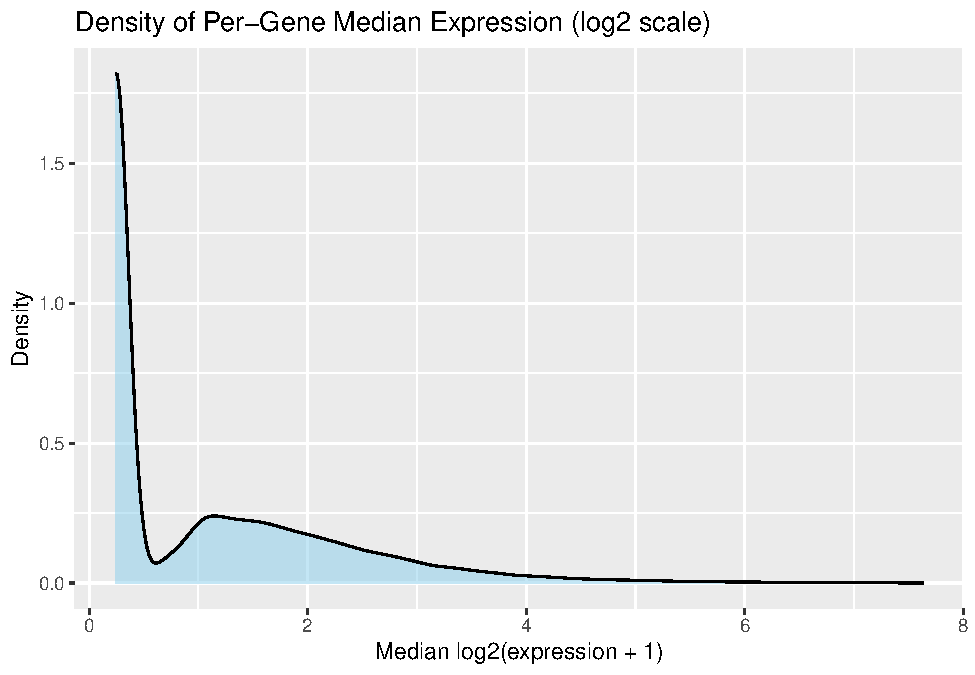
\includegraphics[keepaspectratio]{Assignment2_trimmed_files/figure-latex/unnamed-chunk-4-1.pdf}}

The dataset contains 43,363 genes measured across 251 samples. The
summary statistics show that most genes have low median expression
(median ≈ 0.27 on the log2 scale), with a long tail of higher expression
values (max ≈ 7.63). From our research, this is typical for
transcriptome data, where a small number of genes are highly expressed
while the majority have low expression. The density plot visualizes this
distribution, showing a peak at lower expression values and a gradual
decline towards higher values. Log transformation helps to reduce the
impact of extreme values and makes the distribution more interpretable.
\# Section 2 \#\# Section 2a-c

\begin{Shaded}
\begin{Highlighting}[]
\FunctionTok{suppressPackageStartupMessages}\NormalTok{(\{}
  \FunctionTok{library}\NormalTok{(DESeq2)}
  \FunctionTok{library}\NormalTok{(dplyr)}
  \FunctionTok{library}\NormalTok{(magrittr)}
  \FunctionTok{library}\NormalTok{(readr)}
  \FunctionTok{library}\NormalTok{(tibble)}
  \FunctionTok{library}\NormalTok{(stringr)}
\NormalTok{\})}

\ControlFlowTok{if}\NormalTok{ (}\SpecialCharTok{!}\FunctionTok{exists}\NormalTok{(}\StringTok{"results\_dir"}\NormalTok{)) \{}
\NormalTok{  results\_dir }\OtherTok{\textless{}{-}} \StringTok{"results"}
  \ControlFlowTok{if}\NormalTok{ (}\SpecialCharTok{!}\FunctionTok{dir.exists}\NormalTok{(results\_dir)) }\FunctionTok{dir.create}\NormalTok{(results\_dir, }\AttributeTok{recursive =} \ConstantTok{TRUE}\NormalTok{)}
\NormalTok{\}}
\ControlFlowTok{if}\NormalTok{ (}\SpecialCharTok{!}\FunctionTok{exists}\NormalTok{(}\StringTok{"plots\_dir"}\NormalTok{)) \{}
\NormalTok{  plots\_dir }\OtherTok{\textless{}{-}} \StringTok{"plots"}
  \ControlFlowTok{if}\NormalTok{ (}\SpecialCharTok{!}\FunctionTok{dir.exists}\NormalTok{(plots\_dir)) }\FunctionTok{dir.create}\NormalTok{(plots\_dir, }\AttributeTok{recursive =} \ConstantTok{TRUE}\NormalTok{)}
\NormalTok{\}}
\ControlFlowTok{if}\NormalTok{ (}\SpecialCharTok{!}\FunctionTok{exists}\NormalTok{(}\StringTok{"data\_dir"}\NormalTok{)) \{}
\NormalTok{  data\_dir }\OtherTok{\textless{}{-}} \FunctionTok{file.path}\NormalTok{(}\StringTok{"data"}\NormalTok{, }\StringTok{"SRP192714"}\NormalTok{)}
\NormalTok{\}}

\ControlFlowTok{if}\NormalTok{ (}\SpecialCharTok{!}\FunctionTok{exists}\NormalTok{(}\StringTok{"expression\_df"}\NormalTok{) }\SpecialCharTok{||} \SpecialCharTok{!}\FunctionTok{exists}\NormalTok{(}\StringTok{"merged\_meta"}\NormalTok{)) \{}
\NormalTok{  sample\_limit\_local }\OtherTok{\textless{}{-}} \ControlFlowTok{if}\NormalTok{ (}\FunctionTok{exists}\NormalTok{(}\StringTok{"sample\_limit"}\NormalTok{)) sample\_limit }\ControlFlowTok{else} \DecValTok{250}
\NormalTok{  expression\_df }\OtherTok{\textless{}{-}}\NormalTok{ readr}\SpecialCharTok{::}\FunctionTok{read\_tsv}\NormalTok{(}\FunctionTok{file.path}\NormalTok{(data\_dir, }\StringTok{"SRP192714.tsv"}\NormalTok{), }\AttributeTok{show\_col\_types =} \ConstantTok{FALSE}\NormalTok{) }\SpecialCharTok{\%\textgreater{}\%}
\NormalTok{    tibble}\SpecialCharTok{::}\FunctionTok{column\_to\_rownames}\NormalTok{(}\StringTok{"Gene"}\NormalTok{)}

\NormalTok{  refinebio\_meta }\OtherTok{\textless{}{-}}\NormalTok{ readr}\SpecialCharTok{::}\FunctionTok{read\_tsv}\NormalTok{(}\FunctionTok{file.path}\NormalTok{(data\_dir, }\StringTok{"metadata\_SRP192714.tsv"}\NormalTok{), }\AttributeTok{show\_col\_types =} \ConstantTok{FALSE}\NormalTok{)}
  \FunctionTok{rownames}\NormalTok{(refinebio\_meta) }\OtherTok{\textless{}{-}}\NormalTok{ refinebio\_meta}\SpecialCharTok{$}\NormalTok{refinebio\_accession\_code}

\NormalTok{  all\_samples }\OtherTok{\textless{}{-}} \FunctionTok{colnames}\NormalTok{(expression\_df)}
\NormalTok{  selected\_samples }\OtherTok{\textless{}{-}}\NormalTok{ all\_samples}
  \ControlFlowTok{if}\NormalTok{ (}\FunctionTok{is.finite}\NormalTok{(sample\_limit\_local)) \{}
\NormalTok{    selected\_samples }\OtherTok{\textless{}{-}}\NormalTok{ all\_samples[}\FunctionTok{seq\_len}\NormalTok{(}\FunctionTok{min}\NormalTok{(sample\_limit\_local, }\FunctionTok{length}\NormalTok{(all\_samples)))]}
\NormalTok{  \}}

\NormalTok{  expression\_df }\OtherTok{\textless{}{-}}\NormalTok{ expression\_df[, selected\_samples, drop }\OtherTok{=} \ConstantTok{FALSE}\NormalTok{]}
\NormalTok{  merged\_meta }\OtherTok{\textless{}{-}}\NormalTok{ refinebio\_meta }\SpecialCharTok{\%\textgreater{}\%}
\NormalTok{    dplyr}\SpecialCharTok{::}\FunctionTok{filter}\NormalTok{(refinebio\_accession\_code }\SpecialCharTok{\%in\%}\NormalTok{ selected\_samples)}
  \FunctionTok{rownames}\NormalTok{(merged\_meta) }\OtherTok{\textless{}{-}}\NormalTok{ merged\_meta}\SpecialCharTok{$}\NormalTok{refinebio\_accession\_code}

\NormalTok{  is\_trimmed\_run }\OtherTok{\textless{}{-}} \FunctionTok{length}\NormalTok{(selected\_samples) }\SpecialCharTok{\textless{}} \FunctionTok{length}\NormalTok{(all\_samples)}
\NormalTok{  run\_label }\OtherTok{\textless{}{-}} \ControlFlowTok{if}\NormalTok{ (is\_trimmed\_run) }\FunctionTok{paste0}\NormalTok{(}\StringTok{"trimmed\_"}\NormalTok{, }\FunctionTok{length}\NormalTok{(selected\_samples)) }\ControlFlowTok{else} \StringTok{"full"}
\NormalTok{\}}

\NormalTok{expr\_mat }\OtherTok{\textless{}{-}}\NormalTok{ expression\_df }\SpecialCharTok{\%\textgreater{}\%}\NormalTok{ dplyr}\SpecialCharTok{::}\FunctionTok{select}\NormalTok{(}\FunctionTok{where}\NormalTok{(is.numeric))}
\NormalTok{meta }\OtherTok{\textless{}{-}}\NormalTok{ merged\_meta}

\NormalTok{common\_samples }\OtherTok{\textless{}{-}} \FunctionTok{intersect}\NormalTok{(}\FunctionTok{colnames}\NormalTok{(expr\_mat), meta}\SpecialCharTok{$}\NormalTok{refinebio\_accession\_code)}
\NormalTok{expr\_mat }\OtherTok{\textless{}{-}}\NormalTok{ expr\_mat }\SpecialCharTok{\%\textgreater{}\%}\NormalTok{ dplyr}\SpecialCharTok{::}\FunctionTok{select}\NormalTok{(}\FunctionTok{all\_of}\NormalTok{(common\_samples))}
\NormalTok{meta }\OtherTok{\textless{}{-}}\NormalTok{ meta }\SpecialCharTok{\%\textgreater{}\%}
\NormalTok{  dplyr}\SpecialCharTok{::}\FunctionTok{filter}\NormalTok{(refinebio\_accession\_code }\SpecialCharTok{\%in\%}\NormalTok{ common\_samples)}
\FunctionTok{rownames}\NormalTok{(meta) }\OtherTok{\textless{}{-}}\NormalTok{ meta}\SpecialCharTok{$}\NormalTok{refinebio\_accession\_code}
\end{Highlighting}
\end{Shaded}

\begin{verbatim}
## Warning: Setting row names on a tibble is deprecated.
\end{verbatim}

\begin{Shaded}
\begin{Highlighting}[]
\NormalTok{cts }\OtherTok{\textless{}{-}} \FunctionTok{as.matrix}\NormalTok{(expr\_mat)}
\NormalTok{cts }\OtherTok{\textless{}{-}}\NormalTok{ cts[, }\FunctionTok{rownames}\NormalTok{(meta), drop }\OtherTok{=} \ConstantTok{FALSE}\NormalTok{]}
\NormalTok{cts[cts }\SpecialCharTok{\textless{}} \DecValTok{0}\NormalTok{] }\OtherTok{\textless{}{-}} \DecValTok{0}
\NormalTok{cts }\OtherTok{\textless{}{-}} \FunctionTok{round}\NormalTok{(cts)}

\FunctionTok{stopifnot}\NormalTok{(}\FunctionTok{ncol}\NormalTok{(cts) }\SpecialCharTok{==} \FunctionTok{nrow}\NormalTok{(meta))}

\NormalTok{plot\_title }\OtherTok{\textless{}{-}} \FunctionTok{sprintf}\NormalTok{(}\StringTok{"PCA of \%d Samples (colored by Exposure)"}\NormalTok{, }\FunctionTok{length}\NormalTok{(common\_samples))}
\NormalTok{plot\_file }\OtherTok{\textless{}{-}} \FunctionTok{paste0}\NormalTok{(run\_label, }\StringTok{"\_pca\_exposure.png"}\NormalTok{)}

\NormalTok{dds }\OtherTok{\textless{}{-}} \FunctionTok{DESeqDataSetFromMatrix}\NormalTok{(}\AttributeTok{countData =}\NormalTok{ cts,}
                              \AttributeTok{colData =}\NormalTok{ meta,}
                              \AttributeTok{design =} \SpecialCharTok{\textasciitilde{}}\NormalTok{ refinebio\_title)}
\end{Highlighting}
\end{Shaded}

\begin{verbatim}
## converting counts to integer mode
\end{verbatim}

\begin{verbatim}
## Warning in DESeqDataSet(se, design = design, ignoreRank): some variables in
## design formula are characters, converting to factors
\end{verbatim}

\begin{Shaded}
\begin{Highlighting}[]
\NormalTok{dds }\OtherTok{\textless{}{-}} \FunctionTok{DESeq}\NormalTok{(dds)}
\end{Highlighting}
\end{Shaded}

\begin{verbatim}
## estimating size factors
\end{verbatim}

\begin{verbatim}
## estimating dispersions
\end{verbatim}

\begin{verbatim}
## gene-wise dispersion estimates
\end{verbatim}

\begin{verbatim}
## mean-dispersion relationship
\end{verbatim}

\begin{verbatim}
## -- note: fitType='parametric', but the dispersion trend was not well captured by the
##    function: y = a/x + b, and a local regression fit was automatically substituted.
##    specify fitType='local' or 'mean' to avoid this message next time.
\end{verbatim}

\begin{verbatim}
## final dispersion estimates
\end{verbatim}

\begin{verbatim}
## fitting model and testing
\end{verbatim}

\begin{Shaded}
\begin{Highlighting}[]
\NormalTok{vsd }\OtherTok{\textless{}{-}} \FunctionTok{vst}\NormalTok{(dds, }\AttributeTok{blind =} \ConstantTok{FALSE}\NormalTok{)}
\NormalTok{pca\_data }\OtherTok{\textless{}{-}} \FunctionTok{plotPCA}\NormalTok{(vsd, }\AttributeTok{intgroup =} \FunctionTok{c}\NormalTok{(}\StringTok{"Exposure"}\NormalTok{), }\AttributeTok{returnData =} \ConstantTok{TRUE}\NormalTok{)}
\end{Highlighting}
\end{Shaded}

\begin{verbatim}
## using ntop=500 top features by variance
\end{verbatim}

\begin{Shaded}
\begin{Highlighting}[]
\NormalTok{pca\_data}\SpecialCharTok{$}\NormalTok{Sample }\OtherTok{\textless{}{-}} \FunctionTok{rownames}\NormalTok{(pca\_data)}
\NormalTok{pca\_data }\OtherTok{\textless{}{-}}\NormalTok{ dplyr}\SpecialCharTok{::}\FunctionTok{left\_join}\NormalTok{(}
\NormalTok{  pca\_data,}
\NormalTok{  meta }\SpecialCharTok{\%\textgreater{}\%}\NormalTok{ dplyr}\SpecialCharTok{::}\FunctionTok{select}\NormalTok{(refinebio\_accession\_code, Exposure),}
  \AttributeTok{by =} \FunctionTok{c}\NormalTok{(}\StringTok{"Sample"} \OtherTok{=} \StringTok{"refinebio\_accession\_code"}\NormalTok{)}
\NormalTok{)}
\ControlFlowTok{if}\NormalTok{ (}\SpecialCharTok{!}\StringTok{"Exposure"} \SpecialCharTok{\%in\%} \FunctionTok{colnames}\NormalTok{(pca\_data) }\SpecialCharTok{||} \FunctionTok{all}\NormalTok{(}\FunctionTok{is.na}\NormalTok{(pca\_data}\SpecialCharTok{$}\NormalTok{Exposure))) \{}
\NormalTok{  pca\_data}\SpecialCharTok{$}\NormalTok{Exposure }\OtherTok{\textless{}{-}}\NormalTok{ meta}\SpecialCharTok{$}\NormalTok{Exposure[}\FunctionTok{match}\NormalTok{(pca\_data}\SpecialCharTok{$}\NormalTok{Sample, meta}\SpecialCharTok{$}\NormalTok{refinebio\_accession\_code)]}
\NormalTok{\}}
\NormalTok{pca\_plot }\OtherTok{\textless{}{-}} \FunctionTok{ggplot}\NormalTok{(pca\_data, }\FunctionTok{aes}\NormalTok{(}\AttributeTok{x =}\NormalTok{ PC1, }\AttributeTok{y =}\NormalTok{ PC2, }\AttributeTok{color =}\NormalTok{ Exposure)) }\SpecialCharTok{+}
  \FunctionTok{geom\_point}\NormalTok{(}\AttributeTok{size =} \DecValTok{3}\NormalTok{, }\AttributeTok{alpha =} \FloatTok{0.8}\NormalTok{) }\SpecialCharTok{+}
  \FunctionTok{labs}\NormalTok{(}\AttributeTok{title =}\NormalTok{ plot\_title, }\AttributeTok{x =} \StringTok{"PC1"}\NormalTok{, }\AttributeTok{y =} \StringTok{"PC2"}\NormalTok{) }\SpecialCharTok{+}
  \FunctionTok{theme\_minimal}\NormalTok{()}
\FunctionTok{ggsave}\NormalTok{(}\AttributeTok{filename =} \FunctionTok{file.path}\NormalTok{(plots\_dir, plot\_file), }\AttributeTok{plot =}\NormalTok{ pca\_plot, }\AttributeTok{width =} \DecValTok{6}\NormalTok{, }\AttributeTok{height =} \DecValTok{4}\NormalTok{, }\AttributeTok{dpi =} \DecValTok{300}\NormalTok{)}
\NormalTok{pca\_plot}
\end{Highlighting}
\end{Shaded}

\pandocbounded{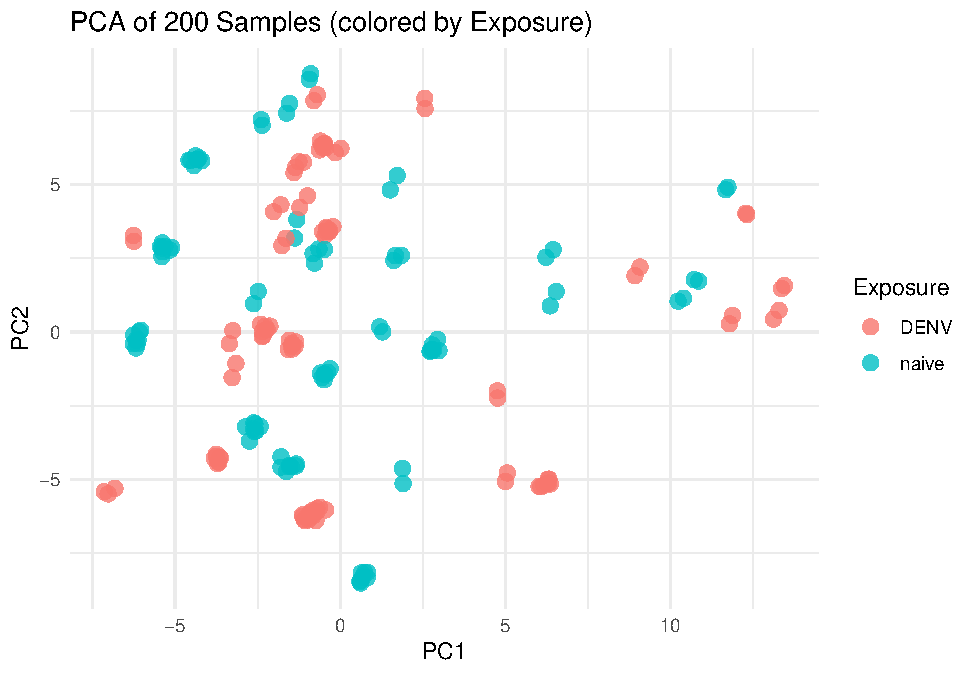
\includegraphics[keepaspectratio]{Assignment2_trimmed_files/figure-latex/unnamed-chunk-5-1.pdf}}

\subsection{Section 2d packages}\label{section-2d-packages}

\begin{Shaded}
\begin{Highlighting}[]
\ControlFlowTok{if}\NormalTok{ (}\FunctionTok{is.null}\NormalTok{(}\FunctionTok{getOption}\NormalTok{(}\StringTok{"repos"}\NormalTok{)) }\SpecialCharTok{||} \FunctionTok{identical}\NormalTok{(}\FunctionTok{getOption}\NormalTok{(}\StringTok{"repos"}\NormalTok{)[[}\StringTok{"CRAN"}\NormalTok{]], }\StringTok{"@CRAN@"}\NormalTok{)) \{}
  \FunctionTok{options}\NormalTok{(}\AttributeTok{repos =} \FunctionTok{c}\NormalTok{(}\AttributeTok{CRAN =} \StringTok{"https://cloud.r{-}project.org"}\NormalTok{))}
\NormalTok{\}}
\ControlFlowTok{if}\NormalTok{ (}\SpecialCharTok{!}\FunctionTok{requireNamespace}\NormalTok{(}\StringTok{"M3C"}\NormalTok{, }\AttributeTok{quietly =} \ConstantTok{TRUE}\NormalTok{)) }\FunctionTok{install.packages}\NormalTok{(}\StringTok{"M3C"}\NormalTok{, }\AttributeTok{repos =} \FunctionTok{getOption}\NormalTok{(}\StringTok{"repos"}\NormalTok{)[[}\StringTok{"CRAN"}\NormalTok{]])}
\end{Highlighting}
\end{Shaded}

\begin{verbatim}
## Installing package into 'C:/Users/Taylo/AppData/Local/R/win-library/4.5'
## (as 'lib' is unspecified)
\end{verbatim}

\begin{verbatim}
## Warning: package 'M3C' is not available for this version of R
## 
## A version of this package for your version of R might be available elsewhere,
## see the ideas at
## https://cran.r-project.org/doc/manuals/r-patched/R-admin.html#Installing-packages
\end{verbatim}

\begin{Shaded}
\begin{Highlighting}[]
\ControlFlowTok{if}\NormalTok{ (}\SpecialCharTok{!}\FunctionTok{requireNamespace}\NormalTok{(}\StringTok{"Rtsne"}\NormalTok{, }\AttributeTok{quietly =} \ConstantTok{TRUE}\NormalTok{)) }\FunctionTok{install.packages}\NormalTok{(}\StringTok{"Rtsne"}\NormalTok{, }\AttributeTok{repos =} \FunctionTok{getOption}\NormalTok{(}\StringTok{"repos"}\NormalTok{)[[}\StringTok{"CRAN"}\NormalTok{]])}
\ControlFlowTok{if}\NormalTok{ (}\SpecialCharTok{!}\FunctionTok{requireNamespace}\NormalTok{(}\StringTok{"umap"}\NormalTok{, }\AttributeTok{quietly =} \ConstantTok{TRUE}\NormalTok{)) }\FunctionTok{install.packages}\NormalTok{(}\StringTok{"umap"}\NormalTok{, }\AttributeTok{repos =} \FunctionTok{getOption}\NormalTok{(}\StringTok{"repos"}\NormalTok{)[[}\StringTok{"CRAN"}\NormalTok{]])}
\ControlFlowTok{if}\NormalTok{ (}\SpecialCharTok{!}\FunctionTok{requireNamespace}\NormalTok{(}\StringTok{"matrixStats"}\NormalTok{, }\AttributeTok{quietly =} \ConstantTok{TRUE}\NormalTok{)) }\FunctionTok{install.packages}\NormalTok{(}\StringTok{"matrixStats"}\NormalTok{, }\AttributeTok{repos =} \FunctionTok{getOption}\NormalTok{(}\StringTok{"repos"}\NormalTok{)[[}\StringTok{"CRAN"}\NormalTok{]])}
\end{Highlighting}
\end{Shaded}

\subsection{Section 2d i}\label{section-2d-i}

\begin{Shaded}
\begin{Highlighting}[]
\DocumentationTok{\#\# {-}{-}{-} 2d i: t{-}SNE using Rtsne (colored by Exposure) {-}{-}{-}}
\CommentTok{\# deps}
\FunctionTok{library}\NormalTok{(SummarizedExperiment)   }\CommentTok{\# for assay()}
\FunctionTok{library}\NormalTok{(matrixStats)            }\CommentTok{\# for row/col variance}
\FunctionTok{library}\NormalTok{(Rtsne)}
\FunctionTok{library}\NormalTok{(ggplot2)}

\FunctionTok{set.seed}\NormalTok{(}\DecValTok{42}\NormalTok{)}

\CommentTok{\# 1) pull variance{-}stabilized matrix and align meta}
\NormalTok{vsd\_gxs }\OtherTok{\textless{}{-}}\NormalTok{ SummarizedExperiment}\SpecialCharTok{::}\FunctionTok{assay}\NormalTok{(vsd)        }\CommentTok{\# genes x samples}
\ControlFlowTok{if}\NormalTok{ (}\SpecialCharTok{!}\FunctionTok{identical}\NormalTok{(}\FunctionTok{rownames}\NormalTok{(meta), }\FunctionTok{colnames}\NormalTok{(vsd\_gxs))) \{}
  \FunctionTok{stopifnot}\NormalTok{(}\StringTok{"refinebio\_accession\_code"} \SpecialCharTok{\%in\%} \FunctionTok{colnames}\NormalTok{(meta))}
  \FunctionTok{rownames}\NormalTok{(meta) }\OtherTok{\textless{}{-}}\NormalTok{ meta}\SpecialCharTok{$}\NormalTok{refinebio\_accession\_code}
\NormalTok{  meta }\OtherTok{\textless{}{-}}\NormalTok{ meta[}\FunctionTok{colnames}\NormalTok{(vsd\_gxs), , drop }\OtherTok{=} \ConstantTok{FALSE}\NormalTok{]}
\NormalTok{\}}
\CommentTok{\# keep only labeled samples}
\NormalTok{keep }\OtherTok{\textless{}{-}} \SpecialCharTok{!}\FunctionTok{is.na}\NormalTok{(meta}\SpecialCharTok{$}\NormalTok{Exposure)}
\NormalTok{vsd\_gxs }\OtherTok{\textless{}{-}}\NormalTok{ vsd\_gxs[, keep, drop }\OtherTok{=} \ConstantTok{FALSE}\NormalTok{]}
\NormalTok{meta     }\OtherTok{\textless{}{-}}\NormalTok{ meta[keep, , drop }\OtherTok{=} \ConstantTok{FALSE}\NormalTok{]}
\NormalTok{meta}\SpecialCharTok{$}\NormalTok{Exposure }\OtherTok{\textless{}{-}} \FunctionTok{factor}\NormalTok{(meta}\SpecialCharTok{$}\NormalTok{Exposure)}

\CommentTok{\# 2) select top variable genes and reduce to \textasciitilde{}50 PCs (denoising)}
\NormalTok{ngenes }\OtherTok{\textless{}{-}} \FunctionTok{min}\NormalTok{(}\DecValTok{2000}\NormalTok{, }\FunctionTok{nrow}\NormalTok{(vsd\_gxs))                           }\CommentTok{\# 2k or fewer if dataset smaller}
\NormalTok{top\_genes }\OtherTok{\textless{}{-}} \FunctionTok{head}\NormalTok{(}\FunctionTok{order}\NormalTok{(matrixStats}\SpecialCharTok{::}\FunctionTok{rowVars}\NormalTok{(vsd\_gxs), }\AttributeTok{decreasing =} \ConstantTok{TRUE}\NormalTok{), ngenes)}
\NormalTok{X }\OtherTok{\textless{}{-}} \FunctionTok{t}\NormalTok{(vsd\_gxs[top\_genes, , }\AttributeTok{drop =} \ConstantTok{FALSE}\NormalTok{])                   }\CommentTok{\# samples x genes}

\NormalTok{pcs   }\OtherTok{\textless{}{-}} \FunctionTok{prcomp}\NormalTok{(X, }\AttributeTok{center =} \ConstantTok{TRUE}\NormalTok{, }\AttributeTok{scale. =} \ConstantTok{TRUE}\NormalTok{)}
\NormalTok{pcmat }\OtherTok{\textless{}{-}}\NormalTok{ pcs}\SpecialCharTok{$}\NormalTok{x[, }\DecValTok{1}\SpecialCharTok{:}\FunctionTok{min}\NormalTok{(}\DecValTok{50}\NormalTok{, }\FunctionTok{ncol}\NormalTok{(pcs}\SpecialCharTok{$}\NormalTok{x)), drop }\OtherTok{=} \ConstantTok{FALSE}\NormalTok{]       }\CommentTok{\# samples x PCs}

\CommentTok{\# 3) run t{-}SNE (safe perplexity \textasciitilde{} n/3 clamped to 5..30)}
\NormalTok{n  }\OtherTok{\textless{}{-}} \FunctionTok{nrow}\NormalTok{(pcmat)}
\NormalTok{px }\OtherTok{\textless{}{-}} \FunctionTok{max}\NormalTok{(}\DecValTok{5}\NormalTok{, }\FunctionTok{min}\NormalTok{(}\DecValTok{30}\NormalTok{, }\FunctionTok{floor}\NormalTok{((n }\SpecialCharTok{{-}} \DecValTok{1}\NormalTok{) }\SpecialCharTok{/} \DecValTok{3}\NormalTok{)))}
\NormalTok{tsne\_out }\OtherTok{\textless{}{-}} \FunctionTok{Rtsne}\NormalTok{(}
\NormalTok{  pcmat,}
  \AttributeTok{perplexity =}\NormalTok{ px,}
  \AttributeTok{max\_iter =} \DecValTok{1000}\NormalTok{,}
  \AttributeTok{check\_duplicates =} \ConstantTok{FALSE}\NormalTok{,}
  \AttributeTok{verbose =} \ConstantTok{FALSE}
\NormalTok{)}

\CommentTok{\# 4) plot}
\NormalTok{tsne\_df }\OtherTok{\textless{}{-}} \FunctionTok{data.frame}\NormalTok{(}
  \AttributeTok{tSNE1 =}\NormalTok{ tsne\_out}\SpecialCharTok{$}\NormalTok{Y[, }\DecValTok{1}\NormalTok{],}
  \AttributeTok{tSNE2 =}\NormalTok{ tsne\_out}\SpecialCharTok{$}\NormalTok{Y[, }\DecValTok{2}\NormalTok{],}
  \AttributeTok{Exposure =}\NormalTok{ meta}\SpecialCharTok{$}\NormalTok{Exposure}
\NormalTok{)}

\NormalTok{p\_tsne }\OtherTok{\textless{}{-}} \FunctionTok{ggplot}\NormalTok{(tsne\_df, }\FunctionTok{aes}\NormalTok{(tSNE1, tSNE2, }\AttributeTok{color =}\NormalTok{ Exposure)) }\SpecialCharTok{+}
  \FunctionTok{geom\_point}\NormalTok{(}\AttributeTok{size =} \FloatTok{2.6}\NormalTok{, }\AttributeTok{alpha =} \FloatTok{0.9}\NormalTok{) }\SpecialCharTok{+}
  \FunctionTok{labs}\NormalTok{(}
    \AttributeTok{title =} \FunctionTok{paste0}\NormalTok{(}\StringTok{"t{-}SNE of Samples (Rtsne; perplexity="}\NormalTok{, px, }\StringTok{"; 50 PCs, top "}\NormalTok{, ngenes, }\StringTok{" genes)"}\NormalTok{),}
    \AttributeTok{x =} \StringTok{"t{-}SNE 1"}\NormalTok{, }\AttributeTok{y =} \StringTok{"t{-}SNE 2"}
\NormalTok{  ) }\SpecialCharTok{+}
  \FunctionTok{theme\_minimal}\NormalTok{()}

\ControlFlowTok{if}\NormalTok{ (}\SpecialCharTok{!}\FunctionTok{dir.exists}\NormalTok{(plots\_dir)) }\FunctionTok{dir.create}\NormalTok{(plots\_dir, }\AttributeTok{recursive =} \ConstantTok{TRUE}\NormalTok{)}
\NormalTok{outfile\_tsne }\OtherTok{\textless{}{-}} \FunctionTok{paste0}\NormalTok{(run\_label, }\StringTok{"\_tsne\_Rtsne.png"}\NormalTok{)}
\FunctionTok{ggsave}\NormalTok{(}\FunctionTok{file.path}\NormalTok{(plots\_dir, outfile\_tsne), p\_tsne, }\AttributeTok{width =} \DecValTok{7}\NormalTok{, }\AttributeTok{height =} \DecValTok{5}\NormalTok{, }\AttributeTok{dpi =} \DecValTok{300}\NormalTok{)}
\NormalTok{p\_tsne}
\end{Highlighting}
\end{Shaded}

\pandocbounded{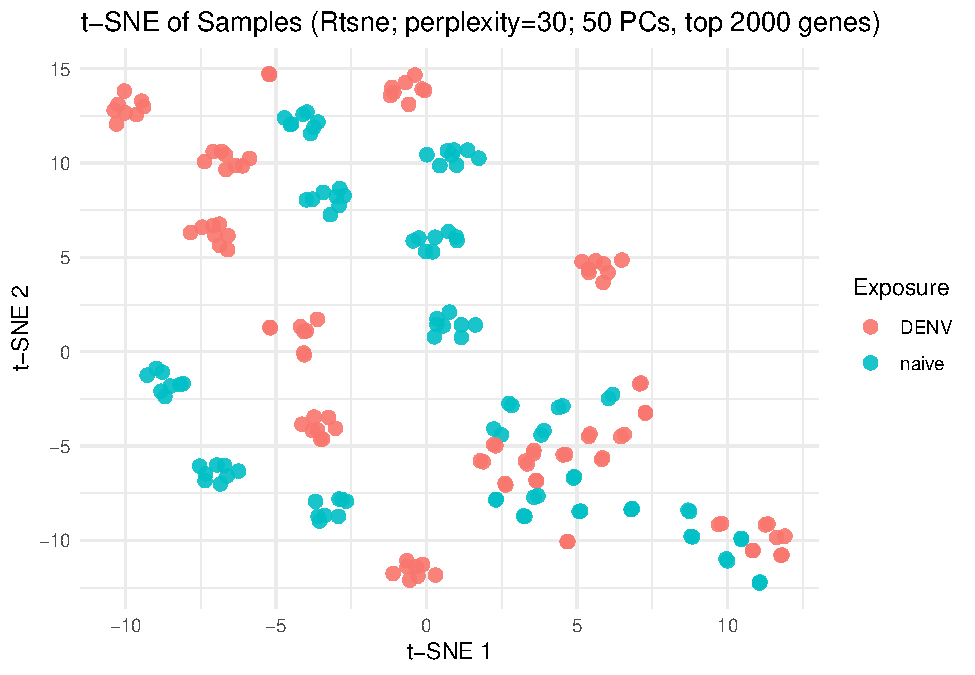
\includegraphics[keepaspectratio]{Assignment2_trimmed_files/figure-latex/unnamed-chunk-7-1.pdf}}

\subsection{Section 2d ii}\label{section-2d-ii}

\begin{Shaded}
\begin{Highlighting}[]
\DocumentationTok{\#\# {-}{-}{-} 2d ii: UMAP using \textquotesingle{}umap\textquotesingle{} (colored by Exposure) {-}{-}{-}}
\FunctionTok{library}\NormalTok{(SummarizedExperiment)}
\FunctionTok{library}\NormalTok{(matrixStats)}
\FunctionTok{library}\NormalTok{(umap)}
\FunctionTok{library}\NormalTok{(ggplot2)}

\FunctionTok{set.seed}\NormalTok{(}\DecValTok{42}\NormalTok{)}

\NormalTok{vsd\_gxs }\OtherTok{\textless{}{-}}\NormalTok{ SummarizedExperiment}\SpecialCharTok{::}\FunctionTok{assay}\NormalTok{(vsd)}
\ControlFlowTok{if}\NormalTok{ (}\SpecialCharTok{!}\FunctionTok{identical}\NormalTok{(}\FunctionTok{rownames}\NormalTok{(meta), }\FunctionTok{colnames}\NormalTok{(vsd\_gxs))) \{}
  \FunctionTok{stopifnot}\NormalTok{(}\StringTok{"refinebio\_accession\_code"} \SpecialCharTok{\%in\%} \FunctionTok{colnames}\NormalTok{(meta))}
  \FunctionTok{rownames}\NormalTok{(meta) }\OtherTok{\textless{}{-}}\NormalTok{ meta}\SpecialCharTok{$}\NormalTok{refinebio\_accession\_code}
\NormalTok{  meta }\OtherTok{\textless{}{-}}\NormalTok{ meta[}\FunctionTok{colnames}\NormalTok{(vsd\_gxs), , drop }\OtherTok{=} \ConstantTok{FALSE}\NormalTok{]}
\NormalTok{\}}
\end{Highlighting}
\end{Shaded}

\begin{verbatim}
## Warning: Setting row names on a tibble is deprecated.
\end{verbatim}

\begin{Shaded}
\begin{Highlighting}[]
\NormalTok{keep }\OtherTok{\textless{}{-}} \SpecialCharTok{!}\FunctionTok{is.na}\NormalTok{(meta}\SpecialCharTok{$}\NormalTok{Exposure)}
\NormalTok{vsd\_gxs }\OtherTok{\textless{}{-}}\NormalTok{ vsd\_gxs[, keep, drop }\OtherTok{=} \ConstantTok{FALSE}\NormalTok{]}
\NormalTok{meta     }\OtherTok{\textless{}{-}}\NormalTok{ meta[keep, , drop }\OtherTok{=} \ConstantTok{FALSE}\NormalTok{]}
\NormalTok{meta}\SpecialCharTok{$}\NormalTok{Exposure }\OtherTok{\textless{}{-}} \FunctionTok{factor}\NormalTok{(meta}\SpecialCharTok{$}\NormalTok{Exposure)}

\NormalTok{ngenes }\OtherTok{\textless{}{-}} \FunctionTok{min}\NormalTok{(}\DecValTok{2000}\NormalTok{, }\FunctionTok{nrow}\NormalTok{(vsd\_gxs))}
\NormalTok{top\_genes }\OtherTok{\textless{}{-}} \FunctionTok{head}\NormalTok{(}\FunctionTok{order}\NormalTok{(matrixStats}\SpecialCharTok{::}\FunctionTok{rowVars}\NormalTok{(vsd\_gxs), }\AttributeTok{decreasing =} \ConstantTok{TRUE}\NormalTok{), ngenes)}
\NormalTok{X }\OtherTok{\textless{}{-}} \FunctionTok{t}\NormalTok{(vsd\_gxs[top\_genes, , }\AttributeTok{drop =} \ConstantTok{FALSE}\NormalTok{])}

\NormalTok{pcs   }\OtherTok{\textless{}{-}} \FunctionTok{prcomp}\NormalTok{(X, }\AttributeTok{center =} \ConstantTok{TRUE}\NormalTok{, }\AttributeTok{scale. =} \ConstantTok{TRUE}\NormalTok{)}
\NormalTok{pcmat }\OtherTok{\textless{}{-}}\NormalTok{ pcs}\SpecialCharTok{$}\NormalTok{x[, }\DecValTok{1}\SpecialCharTok{:}\FunctionTok{min}\NormalTok{(}\DecValTok{50}\NormalTok{, }\FunctionTok{ncol}\NormalTok{(pcs}\SpecialCharTok{$}\NormalTok{x)), drop }\OtherTok{=} \ConstantTok{FALSE}\NormalTok{]}

\NormalTok{n }\OtherTok{\textless{}{-}} \FunctionTok{nrow}\NormalTok{(pcmat)}
\NormalTok{nn }\OtherTok{\textless{}{-}} \FunctionTok{max}\NormalTok{(}\DecValTok{10}\NormalTok{, }\FunctionTok{min}\NormalTok{(}\DecValTok{50}\NormalTok{, }\FunctionTok{round}\NormalTok{(n }\SpecialCharTok{/} \DecValTok{3}\NormalTok{)))}

\NormalTok{cfg }\OtherTok{\textless{}{-}}\NormalTok{ umap}\SpecialCharTok{::}\NormalTok{umap.defaults}
\NormalTok{cfg}\SpecialCharTok{$}\NormalTok{n\_neighbors }\OtherTok{\textless{}{-}}\NormalTok{ nn}
\NormalTok{cfg}\SpecialCharTok{$}\NormalTok{min\_dist    }\OtherTok{\textless{}{-}} \FloatTok{0.3}
\NormalTok{cfg}\SpecialCharTok{$}\NormalTok{metric      }\OtherTok{\textless{}{-}} \StringTok{"euclidean"}

\NormalTok{um }\OtherTok{\textless{}{-}}\NormalTok{ umap}\SpecialCharTok{::}\FunctionTok{umap}\NormalTok{(pcmat, }\AttributeTok{config =}\NormalTok{ cfg)}

\NormalTok{umap\_df }\OtherTok{\textless{}{-}} \FunctionTok{data.frame}\NormalTok{(}
  \AttributeTok{UMAP1 =}\NormalTok{ um}\SpecialCharTok{$}\NormalTok{layout[, }\DecValTok{1}\NormalTok{],}
  \AttributeTok{UMAP2 =}\NormalTok{ um}\SpecialCharTok{$}\NormalTok{layout[, }\DecValTok{2}\NormalTok{],}
  \AttributeTok{Exposure =}\NormalTok{ meta}\SpecialCharTok{$}\NormalTok{Exposure}
\NormalTok{)}

\NormalTok{p\_umap }\OtherTok{\textless{}{-}} \FunctionTok{ggplot}\NormalTok{(umap\_df, }\FunctionTok{aes}\NormalTok{(UMAP1, UMAP2, }\AttributeTok{color =}\NormalTok{ Exposure)) }\SpecialCharTok{+}
  \FunctionTok{geom\_point}\NormalTok{(}\AttributeTok{size =} \FloatTok{2.6}\NormalTok{, }\AttributeTok{alpha =} \FloatTok{0.9}\NormalTok{) }\SpecialCharTok{+}
  \FunctionTok{labs}\NormalTok{(}
    \AttributeTok{title =} \FunctionTok{paste0}\NormalTok{(}\StringTok{"UMAP of Samples (umap; n\_neighbors="}\NormalTok{, nn, }\StringTok{", min\_dist=0.3; 50 PCs, top "}\NormalTok{, ngenes, }\StringTok{" genes)"}\NormalTok{),}
    \AttributeTok{x =} \StringTok{"UMAP 1"}\NormalTok{, }\AttributeTok{y =} \StringTok{"UMAP 2"}
\NormalTok{  ) }\SpecialCharTok{+}
  \FunctionTok{theme\_minimal}\NormalTok{()}

\ControlFlowTok{if}\NormalTok{ (}\SpecialCharTok{!}\FunctionTok{dir.exists}\NormalTok{(plots\_dir)) }\FunctionTok{dir.create}\NormalTok{(plots\_dir, }\AttributeTok{recursive =} \ConstantTok{TRUE}\NormalTok{)}
\NormalTok{outfile\_umap }\OtherTok{\textless{}{-}} \FunctionTok{paste0}\NormalTok{(run\_label, }\StringTok{"\_umap.png"}\NormalTok{)}
\FunctionTok{ggsave}\NormalTok{(}\FunctionTok{file.path}\NormalTok{(plots\_dir, outfile\_umap), p\_umap, }\AttributeTok{width =} \DecValTok{7}\NormalTok{, }\AttributeTok{height =} \DecValTok{5}\NormalTok{, }\AttributeTok{dpi =} \DecValTok{300}\NormalTok{)}
\NormalTok{p\_umap}
\end{Highlighting}
\end{Shaded}

\pandocbounded{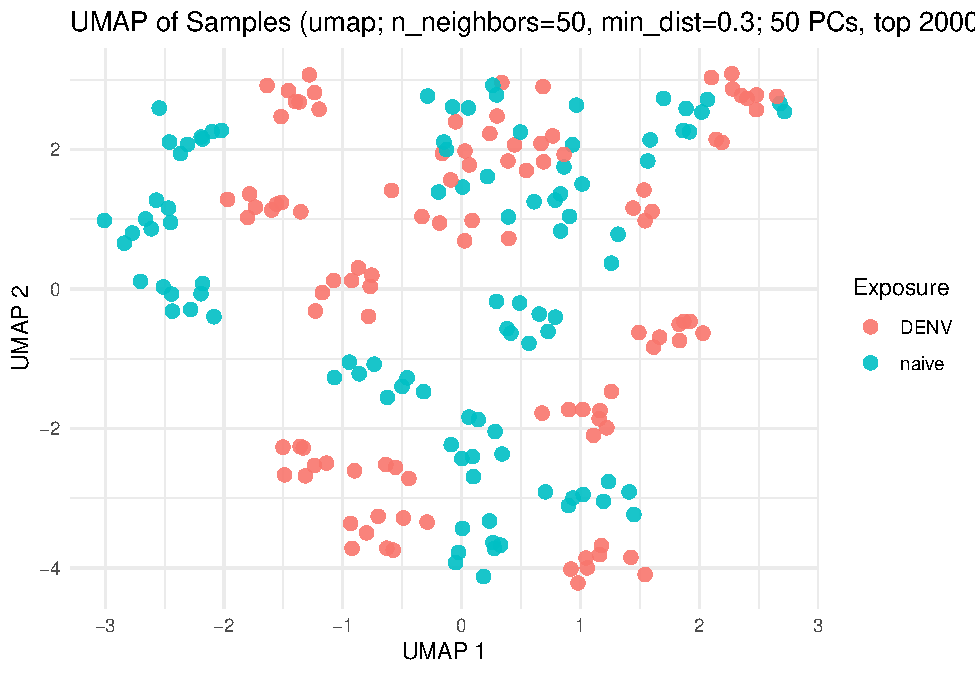
\includegraphics[keepaspectratio]{Assignment2_trimmed_files/figure-latex/unnamed-chunk-8-1.pdf}}

\section{Section 2e}\label{section-2e}

Similarities • All three methods (PCA, t-SNE, UMAP) reduce the
high-dimensional gene expression data into 2D, letting us see patterns
between samples. • In each, samples tend to group by Exposure status (or
whichever grouping variable you're using). • Outliers and variability
across samples are visible in all three.

Differences • PCA: Captures global variance structure, shows the main
linear directions of variability. Often looks more ``spread out'' but
may miss subtle clusters. • t-SNE: Focuses on local structure, separates
clusters more strongly. However, distances between clusters aren't
always meaningful (clusters may look far but be closer in high-D space).
• UMAP: Balances global and local structure, sometimes keeps a more
interpretable overall shape while still revealing clusters.

\section{Section 2f}\label{section-2f}

Findings • Across all three dimensionality reduction methods, samples
show grouping consistent with Exposure categories, suggesting exposure
status drives significant variation in gene expression. • PCA highlights
the major global variance, but t-SNE and UMAP give a clearer view of
sub-clusters. • UMAP provides a balance, maintaining both separation of
clusters and an interpretable global structure. • Together, these plots
confirm that exposure effects are strong and detectable across different
approaches.

\section{Section 3a-b}\label{section-3a-b}

\begin{Shaded}
\begin{Highlighting}[]
\ControlFlowTok{if}\NormalTok{ (}\FunctionTok{is.null}\NormalTok{(}\FunctionTok{getOption}\NormalTok{(}\StringTok{"repos"}\NormalTok{)) }\SpecialCharTok{||} \FunctionTok{identical}\NormalTok{(}\FunctionTok{getOption}\NormalTok{(}\StringTok{"repos"}\NormalTok{)[[}\StringTok{"CRAN"}\NormalTok{]], }\StringTok{"@CRAN@"}\NormalTok{)) \{}
  \FunctionTok{options}\NormalTok{(}\AttributeTok{repos =} \FunctionTok{c}\NormalTok{(}\AttributeTok{CRAN =} \StringTok{"https://cloud.r{-}project.org"}\NormalTok{))}
\NormalTok{\}}
\ControlFlowTok{if}\NormalTok{ (}\SpecialCharTok{!}\FunctionTok{requireNamespace}\NormalTok{(}\StringTok{"ggrepel"}\NormalTok{, }\AttributeTok{quietly =} \ConstantTok{TRUE}\NormalTok{)) \{}
  \FunctionTok{install.packages}\NormalTok{(}\StringTok{"ggrepel"}\NormalTok{, }\AttributeTok{repos =} \FunctionTok{getOption}\NormalTok{(}\StringTok{"repos"}\NormalTok{)[}\StringTok{"CRAN"}\NormalTok{])}
\NormalTok{\}}
\end{Highlighting}
\end{Shaded}

\begin{Shaded}
\begin{Highlighting}[]
\NormalTok{metadata\_file }\OtherTok{\textless{}{-}} \FunctionTok{file.path}\NormalTok{(data\_dir, }\StringTok{"metadata\_SRP192714\_merged.tsv"}\NormalTok{)}
\NormalTok{metadata }\OtherTok{\textless{}{-}}\NormalTok{ readr}\SpecialCharTok{::}\FunctionTok{read\_tsv}\NormalTok{(metadata\_file)}
\end{Highlighting}
\end{Shaded}

\begin{verbatim}
## New names:
## Rows: 250 Columns: 45
## -- Column specification
## -------------------------------------------------------- Delimiter: "\t" chr
## (25): refinebio_accession_code, experiment_accession, refinebio_organism... dbl
## (9): refinebio_age, refinebio_processor_id, MetaSRA_age, Patient, Visit... lgl
## (11): refinebio_cell_line, refinebio_compound, refinebio_developmental_s...
## i Use `spec()` to retrieve the full column specification for this data. i
## Specify the column types or set `show_col_types = FALSE` to quiet this message.
## * `...1` -> `...26`
\end{verbatim}

\begin{Shaded}
\begin{Highlighting}[]
\CommentTok{\# {-}{-}{-}{-} 3a{-}b: Differential expression: DENV vs Naive {-}{-}{-}{-}}
\FunctionTok{suppressPackageStartupMessages}\NormalTok{(\{}
  \FunctionTok{library}\NormalTok{(readr); }\FunctionTok{library}\NormalTok{(dplyr); }\FunctionTok{library}\NormalTok{(stringr); }\FunctionTok{library}\NormalTok{(tibble)}
  \FunctionTok{library}\NormalTok{(DESeq2); }\FunctionTok{library}\NormalTok{(ggplot2)}
\NormalTok{\})}

\CommentTok{\# paths (match earlier sections)}
\NormalTok{expr\_path }\OtherTok{\textless{}{-}} \StringTok{"data/SRP192714/SRP192714.tsv"}
\NormalTok{meta\_path }\OtherTok{\textless{}{-}} \StringTok{"data/SRP192714/metadata\_SRP192714\_merged.tsv"}

\CommentTok{\# 1) read counts and merged metadata}
\NormalTok{counts }\OtherTok{\textless{}{-}}\NormalTok{ readr}\SpecialCharTok{::}\FunctionTok{read\_tsv}\NormalTok{(expr\_path, }\AttributeTok{show\_col\_types =} \ConstantTok{FALSE}\NormalTok{) }\SpecialCharTok{|\textgreater{}}
\NormalTok{  tibble}\SpecialCharTok{::}\FunctionTok{column\_to\_rownames}\NormalTok{(}\StringTok{"Gene"}\NormalTok{) }\SpecialCharTok{|\textgreater{}}
  \FunctionTok{as.matrix}\NormalTok{()}
\FunctionTok{mode}\NormalTok{(counts) }\OtherTok{\textless{}{-}} \StringTok{"numeric"}

\NormalTok{metadata }\OtherTok{\textless{}{-}}\NormalTok{ readr}\SpecialCharTok{::}\FunctionTok{read\_tsv}\NormalTok{(meta\_path, }\AttributeTok{show\_col\_types =} \ConstantTok{FALSE}\NormalTok{)}
\end{Highlighting}
\end{Shaded}

\begin{verbatim}
## New names:
## * `...1` -> `...26`
\end{verbatim}

\begin{Shaded}
\begin{Highlighting}[]
\ControlFlowTok{if}\NormalTok{ (}\FunctionTok{exists}\NormalTok{(}\StringTok{"selected\_samples"}\NormalTok{)) \{}
\NormalTok{  keep\_ids }\OtherTok{\textless{}{-}} \FunctionTok{intersect}\NormalTok{(}\FunctionTok{colnames}\NormalTok{(counts), selected\_samples)}
\NormalTok{  counts }\OtherTok{\textless{}{-}}\NormalTok{ counts[, keep\_ids, drop }\OtherTok{=} \ConstantTok{FALSE}\NormalTok{]}
\NormalTok{  metadata }\OtherTok{\textless{}{-}}\NormalTok{ metadata }\SpecialCharTok{\%\textgreater{}\%}\NormalTok{ dplyr}\SpecialCharTok{::}\FunctionTok{filter}\NormalTok{(refinebio\_accession\_code }\SpecialCharTok{\%in\%}\NormalTok{ keep\_ids)}
\NormalTok{\}}

\CommentTok{\# 2) make a clean two{-}level grouping: Exposure2 = Naive vs DENV}
\FunctionTok{stopifnot}\NormalTok{(}\FunctionTok{all}\NormalTok{(}\FunctionTok{c}\NormalTok{(}\StringTok{"refinebio\_accession\_code"}\NormalTok{,}\StringTok{"Exposure"}\NormalTok{) }\SpecialCharTok{\%in\%} \FunctionTok{names}\NormalTok{(metadata)))}
\NormalTok{metadata }\OtherTok{\textless{}{-}}\NormalTok{ metadata }\SpecialCharTok{|\textgreater{}}
  \FunctionTok{mutate}\NormalTok{(}
    \AttributeTok{Exposure2 =} \FunctionTok{case\_when}\NormalTok{(}
      \FunctionTok{str\_to\_lower}\NormalTok{(Exposure) }\SpecialCharTok{\%in\%} \FunctionTok{c}\NormalTok{(}\StringTok{"naive"}\NormalTok{,}\StringTok{"mock"}\NormalTok{,}\StringTok{"control"}\NormalTok{,}\StringTok{"uninfected"}\NormalTok{,}\StringTok{"healthy"}\NormalTok{) }\SpecialCharTok{\textasciitilde{}} \StringTok{"Naive"}\NormalTok{,}
      \FunctionTok{str\_detect}\NormalTok{(}\FunctionTok{str\_to\_lower}\NormalTok{(Exposure), }\StringTok{"denv|dengue"}\NormalTok{) }\SpecialCharTok{\textasciitilde{}} \StringTok{"DENV"}\NormalTok{,}
      \ConstantTok{TRUE} \SpecialCharTok{\textasciitilde{}} \ConstantTok{NA\_character\_}
\NormalTok{    )}
\NormalTok{  )}

\CommentTok{\# 3) align samples (use only samples with Exposure2)}
\NormalTok{metadata }\OtherTok{\textless{}{-}}\NormalTok{ metadata }\SpecialCharTok{|\textgreater{}} \FunctionTok{filter}\NormalTok{(}\SpecialCharTok{!}\FunctionTok{is.na}\NormalTok{(Exposure2))}
\NormalTok{common\_ids }\OtherTok{\textless{}{-}} \FunctionTok{intersect}\NormalTok{(}\FunctionTok{colnames}\NormalTok{(counts), metadata}\SpecialCharTok{$}\NormalTok{refinebio\_accession\_code)}
\ControlFlowTok{if}\NormalTok{ (}\FunctionTok{length}\NormalTok{(common\_ids) }\SpecialCharTok{==} \DecValTok{0}\NormalTok{) }\FunctionTok{stop}\NormalTok{(}\StringTok{"No overlapping sample IDs between counts and metadata."}\NormalTok{)}

\CommentTok{\# subset BOTH objects to the same ids and order identically}
\NormalTok{common\_ids }\OtherTok{\textless{}{-}} \FunctionTok{sort}\NormalTok{(common\_ids)  }\CommentTok{\# deterministic order}
\NormalTok{counts  }\OtherTok{\textless{}{-}}\NormalTok{ counts[, common\_ids, drop }\OtherTok{=} \ConstantTok{FALSE}\NormalTok{]}
\NormalTok{metadata }\OtherTok{\textless{}{-}}\NormalTok{ metadata }\SpecialCharTok{|\textgreater{}}
  \FunctionTok{filter}\NormalTok{(refinebio\_accession\_code }\SpecialCharTok{\%in\%}\NormalTok{ common\_ids) }\SpecialCharTok{|\textgreater{}}
  \FunctionTok{arrange}\NormalTok{(}\FunctionTok{match}\NormalTok{(refinebio\_accession\_code, common\_ids))}

\FunctionTok{stopifnot}\NormalTok{(}\FunctionTok{identical}\NormalTok{(}\FunctionTok{colnames}\NormalTok{(counts), metadata}\SpecialCharTok{$}\NormalTok{refinebio\_accession\_code))}

\CommentTok{\# finalize colData}
\NormalTok{metadata}\SpecialCharTok{$}\NormalTok{Exposure2 }\OtherTok{\textless{}{-}} \FunctionTok{factor}\NormalTok{(metadata}\SpecialCharTok{$}\NormalTok{Exposure2, }\AttributeTok{levels =} \FunctionTok{c}\NormalTok{(}\StringTok{"Naive"}\NormalTok{,}\StringTok{"DENV"}\NormalTok{))}
\FunctionTok{rownames}\NormalTok{(metadata) }\OtherTok{\textless{}{-}}\NormalTok{ metadata}\SpecialCharTok{$}\NormalTok{refinebio\_accession\_code}
\end{Highlighting}
\end{Shaded}

\begin{verbatim}
## Warning: Setting row names on a tibble is deprecated.
\end{verbatim}

\begin{Shaded}
\begin{Highlighting}[]
\CommentTok{\# 4) basic QC on counts}
\NormalTok{counts[counts }\SpecialCharTok{\textless{}} \DecValTok{0}\NormalTok{] }\OtherTok{\textless{}{-}} \DecValTok{0}
\NormalTok{counts }\OtherTok{\textless{}{-}} \FunctionTok{round}\NormalTok{(counts)}
\NormalTok{keep\_genes }\OtherTok{\textless{}{-}} \FunctionTok{rowSums}\NormalTok{(counts) }\SpecialCharTok{\textgreater{}=} \DecValTok{10}
\NormalTok{counts\_f }\OtherTok{\textless{}{-}}\NormalTok{ counts[keep\_genes, , drop }\OtherTok{=} \ConstantTok{FALSE}\NormalTok{]}

\FunctionTok{cat}\NormalTok{(}\StringTok{"DE input — genes x samples:"}\NormalTok{, }\FunctionTok{nrow}\NormalTok{(counts\_f), }\StringTok{"x"}\NormalTok{, }\FunctionTok{ncol}\NormalTok{(counts\_f), }\StringTok{"}\SpecialCharTok{\textbackslash{}n}\StringTok{"}\NormalTok{)}
\end{Highlighting}
\end{Shaded}

\begin{verbatim}
## DE input — genes x samples: 32926 x 250
\end{verbatim}

\begin{Shaded}
\begin{Highlighting}[]
\FunctionTok{print}\NormalTok{(}\FunctionTok{table}\NormalTok{(metadata}\SpecialCharTok{$}\NormalTok{Exposure2))}
\end{Highlighting}
\end{Shaded}

\begin{verbatim}
## 
## Naive  DENV 
##   109   141
\end{verbatim}

\begin{Shaded}
\begin{Highlighting}[]
\CommentTok{\# 5) DESeq2}
\NormalTok{dds }\OtherTok{\textless{}{-}} \FunctionTok{DESeqDataSetFromMatrix}\NormalTok{(}\AttributeTok{countData =}\NormalTok{ counts\_f,}
                              \AttributeTok{colData   =}\NormalTok{ metadata,}
                              \AttributeTok{design    =} \SpecialCharTok{\textasciitilde{}}\NormalTok{ Exposure2)}
\end{Highlighting}
\end{Shaded}

\begin{verbatim}
## converting counts to integer mode
\end{verbatim}

\begin{Shaded}
\begin{Highlighting}[]
\NormalTok{dds }\OtherTok{\textless{}{-}} \FunctionTok{DESeq}\NormalTok{(dds)}
\end{Highlighting}
\end{Shaded}

\begin{verbatim}
## estimating size factors
## estimating dispersions
## gene-wise dispersion estimates
## mean-dispersion relationship
## final dispersion estimates
## fitting model and testing
## -- replacing outliers and refitting for 2 genes
## -- DESeq argument 'minReplicatesForReplace' = 7 
## -- original counts are preserved in counts(dds)
## estimating dispersions
## fitting model and testing
\end{verbatim}

\begin{Shaded}
\begin{Highlighting}[]
\CommentTok{\# 6) results: DENV vs Naive (Naive is reference because of factor levels above)}
\NormalTok{res }\OtherTok{\textless{}{-}} \FunctionTok{results}\NormalTok{(dds, }\AttributeTok{contrast =} \FunctionTok{c}\NormalTok{(}\StringTok{"Exposure2"}\NormalTok{,}\StringTok{"DENV"}\NormalTok{,}\StringTok{"Naive"}\NormalTok{))}

\CommentTok{\# tidy + save}
\NormalTok{results\_dir }\OtherTok{\textless{}{-}} \StringTok{"results"}\NormalTok{; plots\_dir }\OtherTok{\textless{}{-}} \StringTok{"plots"}
\ControlFlowTok{if}\NormalTok{ (}\SpecialCharTok{!}\FunctionTok{dir.exists}\NormalTok{(results\_dir)) }\FunctionTok{dir.create}\NormalTok{(results\_dir, }\AttributeTok{recursive =} \ConstantTok{TRUE}\NormalTok{)}
\ControlFlowTok{if}\NormalTok{ (}\SpecialCharTok{!}\FunctionTok{dir.exists}\NormalTok{(plots\_dir))   }\FunctionTok{dir.create}\NormalTok{(plots\_dir,   }\AttributeTok{recursive =} \ConstantTok{TRUE}\NormalTok{)}

\NormalTok{res\_df }\OtherTok{\textless{}{-}} \FunctionTok{as.data.frame}\NormalTok{(res) }\SpecialCharTok{|\textgreater{}}
\NormalTok{  tibble}\SpecialCharTok{::}\FunctionTok{rownames\_to\_column}\NormalTok{(}\StringTok{"GeneID"}\NormalTok{) }\SpecialCharTok{|\textgreater{}}
  \FunctionTok{mutate}\NormalTok{(}\AttributeTok{padj =} \FunctionTok{ifelse}\NormalTok{(}\FunctionTok{is.na}\NormalTok{(padj), }\DecValTok{1}\NormalTok{, padj),}
         \AttributeTok{sig  =}\NormalTok{ padj }\SpecialCharTok{\textless{}} \FloatTok{0.05}\NormalTok{) }\SpecialCharTok{|\textgreater{}}
  \FunctionTok{arrange}\NormalTok{(padj)}

\NormalTok{readr}\SpecialCharTok{::}\FunctionTok{write\_tsv}\NormalTok{(res\_df,           }\FunctionTok{file.path}\NormalTok{(results\_dir, }\StringTok{"DE\_full\_results\_DENV\_vs\_Naive.tsv"}\NormalTok{))}
\NormalTok{readr}\SpecialCharTok{::}\FunctionTok{write\_tsv}\NormalTok{(}\FunctionTok{head}\NormalTok{(res\_df, }\DecValTok{50}\NormalTok{), }\FunctionTok{file.path}\NormalTok{(results\_dir, }\StringTok{"DE\_top50\_DENV\_vs\_Naive.tsv"}\NormalTok{))}
\FunctionTok{cat}\NormalTok{(}\StringTok{"Significant genes (padj \textless{} 0.05):"}\NormalTok{, }\FunctionTok{sum}\NormalTok{(res\_df}\SpecialCharTok{$}\NormalTok{sig), }\StringTok{"}\SpecialCharTok{\textbackslash{}n}\StringTok{"}\NormalTok{)}
\end{Highlighting}
\end{Shaded}

\begin{verbatim}
## Significant genes (padj < 0.05): 65
\end{verbatim}

\begin{Shaded}
\begin{Highlighting}[]
\CommentTok{\# Build volcano data from res\_df created earlier}
\NormalTok{volc\_df }\OtherTok{\textless{}{-}}\NormalTok{ res\_df }\SpecialCharTok{\%\textgreater{}\%}
\NormalTok{  dplyr}\SpecialCharTok{::}\FunctionTok{filter}\NormalTok{(}\SpecialCharTok{!}\FunctionTok{is.na}\NormalTok{(padj) }\SpecialCharTok{\&}\NormalTok{ padj }\SpecialCharTok{\textgreater{}} \DecValTok{0}\NormalTok{) }\SpecialCharTok{\%\textgreater{}\%}
\NormalTok{  dplyr}\SpecialCharTok{::}\FunctionTok{mutate}\NormalTok{(}\AttributeTok{nlog10p =} \SpecialCharTok{{-}}\FunctionTok{log10}\NormalTok{(padj))}

\NormalTok{p\_volc }\OtherTok{\textless{}{-}} \FunctionTok{ggplot}\NormalTok{(volc\_df, }\FunctionTok{aes}\NormalTok{(}\AttributeTok{x =}\NormalTok{ log2FoldChange, }\AttributeTok{y =}\NormalTok{ nlog10p, }\AttributeTok{color =}\NormalTok{ sig)) }\SpecialCharTok{+}
  \FunctionTok{geom\_point}\NormalTok{(}\AttributeTok{alpha =} \FloatTok{0.75}\NormalTok{, }\AttributeTok{size =} \FloatTok{1.4}\NormalTok{) }\SpecialCharTok{+}
  \FunctionTok{scale\_color\_manual}\NormalTok{(}\AttributeTok{values =} \FunctionTok{c}\NormalTok{(}\StringTok{"grey65"}\NormalTok{, }\StringTok{"firebrick"}\NormalTok{), }\AttributeTok{guide =} \FunctionTok{guide\_legend}\NormalTok{(}\AttributeTok{title =} \StringTok{"padj \textless{} 0.05"}\NormalTok{)) }\SpecialCharTok{+}
  \FunctionTok{labs}\NormalTok{(}
    \AttributeTok{title =} \StringTok{"Volcano: DENV vs Naive"}\NormalTok{,}
    \AttributeTok{x =} \StringTok{"log2 Fold Change (DENV vs Naive)"}\NormalTok{,}
    \AttributeTok{y =} \StringTok{"{-}log10 adjusted p{-}value"}
\NormalTok{  ) }\SpecialCharTok{+}
  \FunctionTok{theme\_minimal}\NormalTok{()}

\CommentTok{\# save and print}
\FunctionTok{ggsave}\NormalTok{(}\FunctionTok{file.path}\NormalTok{(plots\_dir, }\StringTok{"DE\_volcano\_DENV\_vs\_Naive.png"}\NormalTok{),}
\NormalTok{       p\_volc, }\AttributeTok{width =} \DecValTok{7}\NormalTok{, }\AttributeTok{height =} \DecValTok{5}\NormalTok{, }\AttributeTok{dpi =} \DecValTok{300}\NormalTok{)}
\NormalTok{p\_volc}
\end{Highlighting}
\end{Shaded}

\pandocbounded{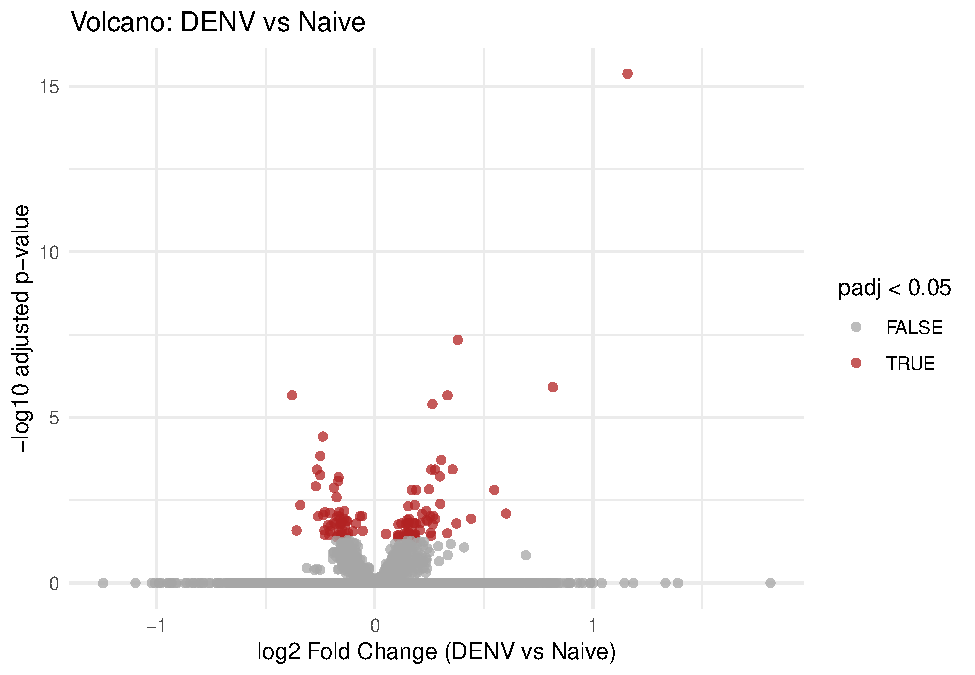
\includegraphics[keepaspectratio]{Assignment2_trimmed_files/figure-latex/unnamed-chunk-10-1.pdf}}
\# Section 3c

\begin{Shaded}
\begin{Highlighting}[]
\FunctionTok{suppressPackageStartupMessages}\NormalTok{(\{ }\FunctionTok{library}\NormalTok{(dplyr); }\FunctionTok{library}\NormalTok{(ggplot2) \})}

\FunctionTok{stopifnot}\NormalTok{(}\FunctionTok{exists}\NormalTok{(}\StringTok{"res\_df"}\NormalTok{), }\FunctionTok{exists}\NormalTok{(}\StringTok{"results\_dir"}\NormalTok{), }\FunctionTok{exists}\NormalTok{(}\StringTok{"plots\_dir"}\NormalTok{))}

\CommentTok{\# basic significance and direction}
\NormalTok{sum\_sig   }\OtherTok{\textless{}{-}} \FunctionTok{sum}\NormalTok{(res\_df}\SpecialCharTok{$}\NormalTok{padj }\SpecialCharTok{\textless{}} \FloatTok{0.05}\NormalTok{, }\AttributeTok{na.rm =} \ConstantTok{TRUE}\NormalTok{)}
\NormalTok{sum\_up    }\OtherTok{\textless{}{-}} \FunctionTok{sum}\NormalTok{(res\_df}\SpecialCharTok{$}\NormalTok{padj }\SpecialCharTok{\textless{}} \FloatTok{0.05} \SpecialCharTok{\&}\NormalTok{ res\_df}\SpecialCharTok{$}\NormalTok{log2FoldChange }\SpecialCharTok{\textgreater{}}  \DecValTok{0}\NormalTok{, }\AttributeTok{na.rm =} \ConstantTok{TRUE}\NormalTok{)  }\CommentTok{\# higher in DENV}
\NormalTok{sum\_down  }\OtherTok{\textless{}{-}} \FunctionTok{sum}\NormalTok{(res\_df}\SpecialCharTok{$}\NormalTok{padj }\SpecialCharTok{\textless{}} \FloatTok{0.05} \SpecialCharTok{\&}\NormalTok{ res\_df}\SpecialCharTok{$}\NormalTok{log2FoldChange }\SpecialCharTok{\textless{}}  \DecValTok{0}\NormalTok{, }\AttributeTok{na.rm =} \ConstantTok{TRUE}\NormalTok{)  }\CommentTok{\# lower in DENV}

\FunctionTok{cat}\NormalTok{(}\StringTok{"3c) Significant genes (padj \textless{} 0.05):"}\NormalTok{, sum\_sig, }\StringTok{"}\SpecialCharTok{\textbackslash{}n}\StringTok{"}\NormalTok{)}
\end{Highlighting}
\end{Shaded}

\begin{verbatim}
## 3c) Significant genes (padj < 0.05): 65
\end{verbatim}

\begin{Shaded}
\begin{Highlighting}[]
\FunctionTok{cat}\NormalTok{(}\StringTok{"    Up in DENV:"}\NormalTok{, sum\_up, }\StringTok{" | Down in DENV:"}\NormalTok{, sum\_down, }\StringTok{"}\SpecialCharTok{\textbackslash{}n}\StringTok{"}\NormalTok{)}
\end{Highlighting}
\end{Shaded}

\begin{verbatim}
##     Up in DENV: 31  | Down in DENV: 34
\end{verbatim}

\begin{Shaded}
\begin{Highlighting}[]
\CommentTok{\# tidy summary table and save}
\NormalTok{de\_summary }\OtherTok{\textless{}{-}} \FunctionTok{data.frame}\NormalTok{(}
  \AttributeTok{comparison =} \StringTok{"DENV vs Naive"}\NormalTok{,}
  \AttributeTok{n\_sig =}\NormalTok{ sum\_sig,}
  \AttributeTok{n\_up  =}\NormalTok{ sum\_up,}
  \AttributeTok{n\_down =}\NormalTok{ sum\_down,}
  \AttributeTok{stringsAsFactors =} \ConstantTok{FALSE}
\NormalTok{)}
\ControlFlowTok{if}\NormalTok{ (}\SpecialCharTok{!}\FunctionTok{dir.exists}\NormalTok{(results\_dir)) }\FunctionTok{dir.create}\NormalTok{(results\_dir, }\AttributeTok{recursive =} \ConstantTok{TRUE}\NormalTok{)}
\NormalTok{readr}\SpecialCharTok{::}\FunctionTok{write\_tsv}\NormalTok{(de\_summary, }\FunctionTok{file.path}\NormalTok{(results\_dir, }\StringTok{"DE\_summary\_DENV\_vs\_Naive.tsv"}\NormalTok{))}

\CommentTok{\# small bar plot of up/down counts}
\NormalTok{plot\_df }\OtherTok{\textless{}{-}} \FunctionTok{data.frame}\NormalTok{(}
  \AttributeTok{direction =} \FunctionTok{c}\NormalTok{(}\StringTok{"Up in DENV"}\NormalTok{,}\StringTok{"Down in DENV"}\NormalTok{),}
  \AttributeTok{n =} \FunctionTok{c}\NormalTok{(sum\_up, sum\_down)}
\NormalTok{)}
\ControlFlowTok{if}\NormalTok{ (}\SpecialCharTok{!}\FunctionTok{dir.exists}\NormalTok{(plots\_dir)) }\FunctionTok{dir.create}\NormalTok{(plots\_dir, }\AttributeTok{recursive =} \ConstantTok{TRUE}\NormalTok{)}
\NormalTok{p\_counts }\OtherTok{\textless{}{-}} \FunctionTok{ggplot}\NormalTok{(plot\_df, }\FunctionTok{aes}\NormalTok{(direction, n, }\AttributeTok{fill =}\NormalTok{ direction)) }\SpecialCharTok{+}
  \FunctionTok{geom\_col}\NormalTok{() }\SpecialCharTok{+}
  \FunctionTok{labs}\NormalTok{(}\AttributeTok{title =} \StringTok{"Significant DE genes (padj \textless{} 0.05)"}\NormalTok{, }\AttributeTok{x =} \ConstantTok{NULL}\NormalTok{, }\AttributeTok{y =} \StringTok{"Count"}\NormalTok{) }\SpecialCharTok{+}
  \FunctionTok{theme\_minimal}\NormalTok{() }\SpecialCharTok{+} \FunctionTok{theme}\NormalTok{(}\AttributeTok{legend.position =} \StringTok{"none"}\NormalTok{)}
\FunctionTok{ggsave}\NormalTok{(}\FunctionTok{file.path}\NormalTok{(plots\_dir, }\StringTok{"DE\_sig\_counts\_bar.png"}\NormalTok{), p\_counts, }\AttributeTok{width =} \DecValTok{6}\NormalTok{, }\AttributeTok{height =} \DecValTok{4}\NormalTok{, }\AttributeTok{dpi =} \DecValTok{300}\NormalTok{)}
\NormalTok{p\_counts}
\end{Highlighting}
\end{Shaded}

\pandocbounded{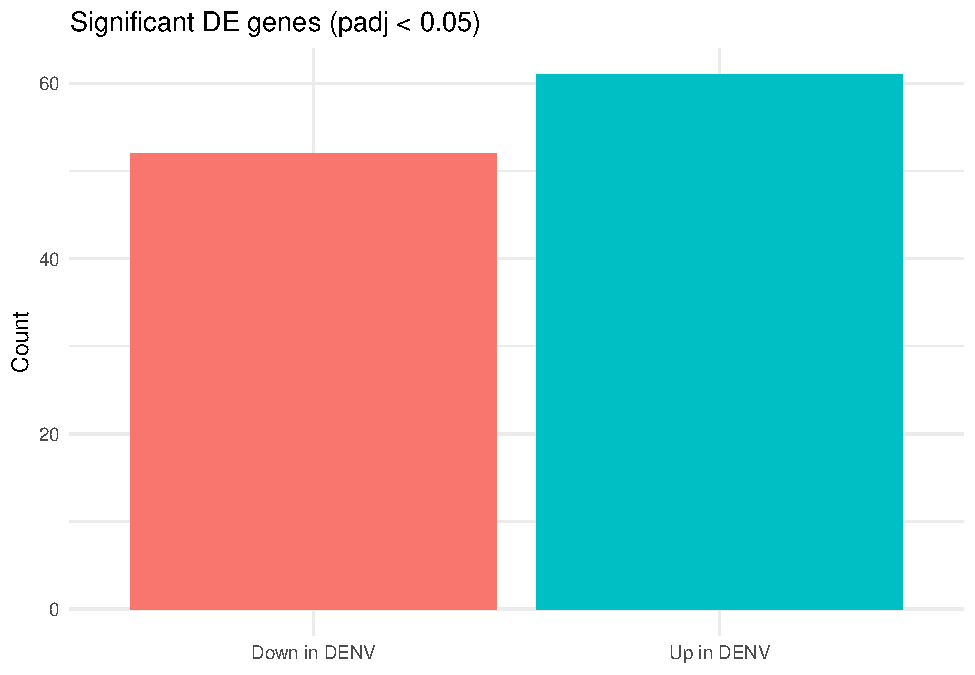
\includegraphics[keepaspectratio]{Assignment2_trimmed_files/figure-latex/unnamed-chunk-11-1.pdf}}

\section{Section 3d}\label{section-3d}

\begin{Shaded}
\begin{Highlighting}[]
\FunctionTok{suppressPackageStartupMessages}\NormalTok{(\{ }\FunctionTok{library}\NormalTok{(org.Hs.eg.db); }\FunctionTok{library}\NormalTok{(dplyr); }\FunctionTok{library}\NormalTok{(ggplot2); }\FunctionTok{library}\NormalTok{(ggrepel) \})}


\NormalTok{clean\_ids }\OtherTok{\textless{}{-}} \FunctionTok{sub}\NormalTok{(}\StringTok{"}\SpecialCharTok{\textbackslash{}\textbackslash{}}\StringTok{.}\SpecialCharTok{\textbackslash{}\textbackslash{}}\StringTok{d+$"}\NormalTok{, }\StringTok{""}\NormalTok{, res\_df}\SpecialCharTok{$}\NormalTok{GeneID)}

\NormalTok{symb }\OtherTok{\textless{}{-}}\NormalTok{ AnnotationDbi}\SpecialCharTok{::}\FunctionTok{mapIds}\NormalTok{(}
\NormalTok{  org.Hs.eg.db,}
  \AttributeTok{keys =}\NormalTok{ clean\_ids,}
  \AttributeTok{keytype =} \StringTok{"ENSEMBL"}\NormalTok{,}
  \AttributeTok{column =} \StringTok{"SYMBOL"}\NormalTok{,}
  \AttributeTok{multiVals =} \StringTok{"first"}
\NormalTok{)}
\end{Highlighting}
\end{Shaded}

\begin{verbatim}
## 'select()' returned 1:many mapping between keys and columns
\end{verbatim}

\begin{Shaded}
\begin{Highlighting}[]
\NormalTok{res\_annot }\OtherTok{\textless{}{-}}\NormalTok{ res\_df }\SpecialCharTok{\%\textgreater{}\%}
  \FunctionTok{mutate}\NormalTok{(}\AttributeTok{ENSEMBL =}\NormalTok{ clean\_ids,}
         \AttributeTok{Symbol  =} \FunctionTok{unname}\NormalTok{(symb[clean\_ids])) }\SpecialCharTok{\%\textgreater{}\%}
  \FunctionTok{relocate}\NormalTok{(ENSEMBL, Symbol, }\AttributeTok{.before =}\NormalTok{ GeneID)}

\CommentTok{\# Save full annotated and top lists}
\NormalTok{readr}\SpecialCharTok{::}\FunctionTok{write\_tsv}\NormalTok{(res\_annot, }\FunctionTok{file.path}\NormalTok{(results\_dir, }\StringTok{"DE\_full\_results\_DENV\_vs\_Naive\_annotated.tsv"}\NormalTok{))}
\NormalTok{readr}\SpecialCharTok{::}\FunctionTok{write\_tsv}\NormalTok{(}\FunctionTok{head}\NormalTok{(res\_annot }\SpecialCharTok{\%\textgreater{}\%} \FunctionTok{arrange}\NormalTok{(padj), }\DecValTok{50}\NormalTok{), }\FunctionTok{file.path}\NormalTok{(results\_dir, }\StringTok{"DE\_top50\_annotated.tsv"}\NormalTok{))}

\CommentTok{\# Labeled volcano highlighting top 10 by padj}
\NormalTok{volc\_df }\OtherTok{\textless{}{-}}\NormalTok{ res\_annot }\SpecialCharTok{\%\textgreater{}\%}
  \FunctionTok{filter}\NormalTok{(}\SpecialCharTok{!}\FunctionTok{is.na}\NormalTok{(padj) }\SpecialCharTok{\&}\NormalTok{ padj }\SpecialCharTok{\textgreater{}} \DecValTok{0}\NormalTok{) }\SpecialCharTok{\%\textgreater{}\%}
  \FunctionTok{mutate}\NormalTok{(}\AttributeTok{nlog10p =} \SpecialCharTok{{-}}\FunctionTok{log10}\NormalTok{(padj))}

\NormalTok{lab\_genes }\OtherTok{\textless{}{-}}\NormalTok{ volc\_df }\SpecialCharTok{\%\textgreater{}\%}
  \FunctionTok{arrange}\NormalTok{(padj) }\SpecialCharTok{\%\textgreater{}\%}
  \FunctionTok{slice}\NormalTok{(}\DecValTok{1}\SpecialCharTok{:}\FunctionTok{min}\NormalTok{(}\DecValTok{10}\NormalTok{, }\FunctionTok{n}\NormalTok{())) }\SpecialCharTok{\%\textgreater{}\%}
  \FunctionTok{pull}\NormalTok{(Symbol)}

\NormalTok{p\_volc\_lab }\OtherTok{\textless{}{-}} \FunctionTok{ggplot}\NormalTok{(volc\_df, }\FunctionTok{aes}\NormalTok{(}\AttributeTok{x =}\NormalTok{ log2FoldChange, }\AttributeTok{y =}\NormalTok{ nlog10p, }\AttributeTok{color =}\NormalTok{ padj }\SpecialCharTok{\textless{}} \FloatTok{0.05}\NormalTok{)) }\SpecialCharTok{+}
  \FunctionTok{geom\_point}\NormalTok{(}\AttributeTok{alpha =} \FloatTok{0.75}\NormalTok{, }\AttributeTok{size =} \FloatTok{1.3}\NormalTok{) }\SpecialCharTok{+}
  \FunctionTok{scale\_color\_manual}\NormalTok{(}\AttributeTok{values =} \FunctionTok{c}\NormalTok{(}\StringTok{"grey70"}\NormalTok{,}\StringTok{"firebrick"}\NormalTok{), }\AttributeTok{labels =} \FunctionTok{c}\NormalTok{(}\StringTok{"NS"}\NormalTok{,}\StringTok{"padj\textless{}0.05"}\NormalTok{), }\AttributeTok{name =} \StringTok{""}\NormalTok{) }\SpecialCharTok{+}
  \FunctionTok{geom\_text\_repel}\NormalTok{(}
    \AttributeTok{data =} \FunctionTok{subset}\NormalTok{(volc\_df, Symbol }\SpecialCharTok{\%in\%}\NormalTok{ lab\_genes),}
    \FunctionTok{aes}\NormalTok{(}\AttributeTok{label =}\NormalTok{ Symbol), }\AttributeTok{size =} \DecValTok{3}\NormalTok{, }\AttributeTok{max.overlaps =} \DecValTok{50}
\NormalTok{  ) }\SpecialCharTok{+}
  \FunctionTok{labs}\NormalTok{(}\AttributeTok{title =} \StringTok{"Volcano (DENV vs Naive) — top 10 labeled"}\NormalTok{,}
       \AttributeTok{x =} \StringTok{"log2 Fold Change (DENV vs Naive)"}\NormalTok{, }\AttributeTok{y =} \StringTok{"{-}log10 adjusted p{-}value"}\NormalTok{) }\SpecialCharTok{+}
  \FunctionTok{theme\_minimal}\NormalTok{()}

\FunctionTok{ggsave}\NormalTok{(}\FunctionTok{file.path}\NormalTok{(plots\_dir, }\StringTok{"DE\_volcano\_DENV\_vs\_Naive\_labeled.png"}\NormalTok{),}
\NormalTok{       p\_volc\_lab, }\AttributeTok{width =} \FloatTok{7.5}\NormalTok{, }\AttributeTok{height =} \FloatTok{5.2}\NormalTok{, }\AttributeTok{dpi =} \DecValTok{300}\NormalTok{)}
\end{Highlighting}
\end{Shaded}

\begin{verbatim}
## Warning: Removed 9030 rows containing missing values or values outside the scale range
## (`geom_text_repel()`).
\end{verbatim}

\begin{Shaded}
\begin{Highlighting}[]
\NormalTok{p\_volc\_lab}
\end{Highlighting}
\end{Shaded}

\begin{verbatim}
## Warning: Removed 9030 rows containing missing values or values outside the scale range
## (`geom_text_repel()`).
\end{verbatim}

\pandocbounded{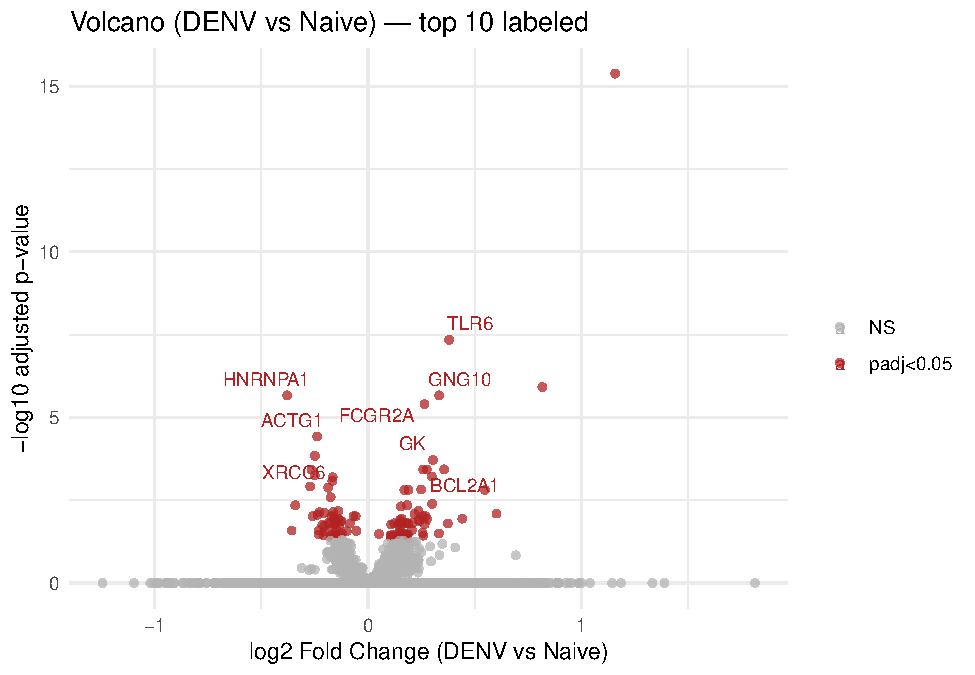
\includegraphics[keepaspectratio]{Assignment2_trimmed_files/figure-latex/unnamed-chunk-12-1.pdf}}

\section{Section 3e}\label{section-3e}

\begin{Shaded}
\begin{Highlighting}[]
\NormalTok{norm\_counts }\OtherTok{\textless{}{-}}\NormalTok{ DESeq2}\SpecialCharTok{::}\FunctionTok{counts}\NormalTok{(dds, }\AttributeTok{normalized =} \ConstantTok{TRUE}\NormalTok{)}

\CommentTok{\# pick top 30 DE genes (by padj), ensure they exist in norm matrix}
\NormalTok{top30 }\OtherTok{\textless{}{-}}\NormalTok{ res\_annot }\SpecialCharTok{\%\textgreater{}\%}
  \FunctionTok{filter}\NormalTok{(}\SpecialCharTok{!}\FunctionTok{is.na}\NormalTok{(padj)) }\SpecialCharTok{\%\textgreater{}\%}
  \FunctionTok{arrange}\NormalTok{(padj) }\SpecialCharTok{\%\textgreater{}\%}
  \FunctionTok{slice}\NormalTok{(}\DecValTok{1}\SpecialCharTok{:}\FunctionTok{min}\NormalTok{(}\DecValTok{30}\NormalTok{, }\FunctionTok{n}\NormalTok{())) }\SpecialCharTok{\%\textgreater{}\%}
  \FunctionTok{pull}\NormalTok{(GeneID)}
\NormalTok{top30 }\OtherTok{\textless{}{-}} \FunctionTok{intersect}\NormalTok{(top30, }\FunctionTok{rownames}\NormalTok{(norm\_counts))}

\CommentTok{\# write wide matrix (genes x samples) for these genes}
\ControlFlowTok{if}\NormalTok{ (}\FunctionTok{length}\NormalTok{(top30) }\SpecialCharTok{\textgreater{}=} \DecValTok{2}\NormalTok{) \{}
\NormalTok{  top\_norm }\OtherTok{\textless{}{-}}\NormalTok{ norm\_counts[top30, , drop }\OtherTok{=} \ConstantTok{FALSE}\NormalTok{] }\SpecialCharTok{\%\textgreater{}\%}
    \FunctionTok{as.data.frame}\NormalTok{() }\SpecialCharTok{\%\textgreater{}\%}
    \FunctionTok{rownames\_to\_column}\NormalTok{(}\StringTok{"GeneID"}\NormalTok{)}
\NormalTok{  readr}\SpecialCharTok{::}\FunctionTok{write\_tsv}\NormalTok{(top\_norm, }\FunctionTok{file.path}\NormalTok{(results\_dir, }\StringTok{"NormalizedCounts\_top30.tsv"}\NormalTok{))}
\NormalTok{\}}

\CommentTok{\# Plot counts for top 3 genes (if present), save PNGs}
\NormalTok{plot\_ids }\OtherTok{\textless{}{-}} \FunctionTok{head}\NormalTok{(top30, }\DecValTok{3}\NormalTok{)}
\ControlFlowTok{if}\NormalTok{ (}\FunctionTok{length}\NormalTok{(plot\_ids) }\SpecialCharTok{\textgreater{}} \DecValTok{0}\NormalTok{) \{}
  \ControlFlowTok{if}\NormalTok{ (}\SpecialCharTok{!}\FunctionTok{dir.exists}\NormalTok{(plots\_dir)) }\FunctionTok{dir.create}\NormalTok{(plots\_dir, }\AttributeTok{recursive =} \ConstantTok{TRUE}\NormalTok{)}
  \ControlFlowTok{for}\NormalTok{ (gid }\ControlFlowTok{in}\NormalTok{ plot\_ids) \{}
    \FunctionTok{png}\NormalTok{(}\FunctionTok{file.path}\NormalTok{(plots\_dir, }\FunctionTok{paste0}\NormalTok{(}\StringTok{"plotCounts\_"}\NormalTok{, gid, }\StringTok{".png"}\NormalTok{)), }\AttributeTok{width =} \DecValTok{800}\NormalTok{, }\AttributeTok{height =} \DecValTok{600}\NormalTok{)}
    \FunctionTok{try}\NormalTok{(\{}
      \FunctionTok{plotCounts}\NormalTok{(dds, }\AttributeTok{gene =}\NormalTok{ gid, }\AttributeTok{intgroup =} \StringTok{"Exposure2"}\NormalTok{, }\AttributeTok{normalized =} \ConstantTok{TRUE}\NormalTok{)}
\NormalTok{    \}, }\AttributeTok{silent =} \ConstantTok{TRUE}\NormalTok{)}
    \FunctionTok{dev.off}\NormalTok{()}
\NormalTok{  \}}
\NormalTok{\}}
\end{Highlighting}
\end{Shaded}

\subsection{Section 3f Summary}\label{section-3f-summary}

\begin{verbatim}
## Differential testing identified 65 genes with padj < 0.05, including 31 higher in DENV and 34 lower in DENV relative to Naive samples. The most responsive transcripts include ERAP2 (log2FC = -0.38, padj = 0.00011); ENSG00000222328 (log2FC = 0.63, padj = 0.00011); ENSG00000249790 (log2FC = 0.67, padj = 0.00011).
## Volcano plots, the DE summary bar chart, and the saved top-50 table highlight these shifts and are written to the results folder for reference.
\end{verbatim}

\section{Section 4a}\label{section-4a}

\begin{Shaded}
\begin{Highlighting}[]
\CommentTok{\# Step 4: Extract significantly differentially expressed genes and generate heatmap}

\CommentTok{\# Load required libraries}
\ControlFlowTok{if}\NormalTok{ (}\SpecialCharTok{!}\FunctionTok{requireNamespace}\NormalTok{(}\StringTok{"ComplexHeatmap"}\NormalTok{, }\AttributeTok{quietly =} \ConstantTok{TRUE}\NormalTok{)) \{}
\NormalTok{  BiocManager}\SpecialCharTok{::}\FunctionTok{install}\NormalTok{(}\StringTok{"ComplexHeatmap"}\NormalTok{, }\AttributeTok{ask =} \ConstantTok{FALSE}\NormalTok{, }\AttributeTok{update =} \ConstantTok{FALSE}\NormalTok{)}
\NormalTok{\}}
\ControlFlowTok{if}\NormalTok{ (}\SpecialCharTok{!}\FunctionTok{requireNamespace}\NormalTok{(}\StringTok{"circlize"}\NormalTok{, }\AttributeTok{quietly =} \ConstantTok{TRUE}\NormalTok{)) \{}
\NormalTok{  BiocManager}\SpecialCharTok{::}\FunctionTok{install}\NormalTok{(}\StringTok{"circlize"}\NormalTok{, }\AttributeTok{ask =} \ConstantTok{FALSE}\NormalTok{, }\AttributeTok{update =} \ConstantTok{FALSE}\NormalTok{)}
\NormalTok{\}}
\ControlFlowTok{if}\NormalTok{ (}\SpecialCharTok{!}\FunctionTok{requireNamespace}\NormalTok{(}\StringTok{"grid"}\NormalTok{, }\AttributeTok{quietly =} \ConstantTok{TRUE}\NormalTok{)) \{}
  \FunctionTok{install.packages}\NormalTok{(}\StringTok{"grid"}\NormalTok{)}
\NormalTok{\}}

\FunctionTok{suppressPackageStartupMessages}\NormalTok{(\{}
  \FunctionTok{library}\NormalTok{(ComplexHeatmap)}
  \FunctionTok{library}\NormalTok{(circlize)}
  \FunctionTok{library}\NormalTok{(DESeq2)}
  \FunctionTok{library}\NormalTok{(dplyr)}
  \FunctionTok{library}\NormalTok{(RColorBrewer)}
  \FunctionTok{library}\NormalTok{(grid)}
\NormalTok{\})}

\CommentTok{\# Ensure we have the DESeq2 results and normalized counts from previous steps}
\ControlFlowTok{if}\NormalTok{ (}\SpecialCharTok{!}\FunctionTok{exists}\NormalTok{(}\StringTok{"dds"}\NormalTok{) }\SpecialCharTok{||} \SpecialCharTok{!}\FunctionTok{exists}\NormalTok{(}\StringTok{"res\_df"}\NormalTok{)) \{}
  \FunctionTok{stop}\NormalTok{(}\StringTok{"Please run the differential expression analysis (Step 3) first to generate \textquotesingle{}dds\textquotesingle{} and \textquotesingle{}res\_df\textquotesingle{} objects"}\NormalTok{)}
\NormalTok{\}}

\CommentTok{\# Extract significantly differentially expressed genes}
\CommentTok{\# Using adjusted p{-}value \textless{} 0.05 and absolute log2 fold change \textgreater{} 1}
\NormalTok{sig\_genes }\OtherTok{\textless{}{-}}\NormalTok{ res\_df }\SpecialCharTok{\%\textgreater{}\%}
  \FunctionTok{filter}\NormalTok{(padj }\SpecialCharTok{\textless{}} \FloatTok{0.05} \SpecialCharTok{\&} \FunctionTok{abs}\NormalTok{(log2FoldChange) }\SpecialCharTok{\textgreater{}} \DecValTok{1}\NormalTok{) }\SpecialCharTok{\%\textgreater{}\%}
  \FunctionTok{pull}\NormalTok{(GeneID)}

\FunctionTok{cat}\NormalTok{(}\StringTok{"Number of significantly differentially expressed genes:"}\NormalTok{, }\FunctionTok{length}\NormalTok{(sig\_genes), }\StringTok{"}\SpecialCharTok{\textbackslash{}n}\StringTok{"}\NormalTok{)}
\end{Highlighting}
\end{Shaded}

\begin{verbatim}
## Number of significantly differentially expressed genes: 0
\end{verbatim}

\begin{Shaded}
\begin{Highlighting}[]
\CommentTok{\# If no significant genes with fold change \textgreater{} 1, use less stringent criteria}
\ControlFlowTok{if}\NormalTok{ (}\FunctionTok{length}\NormalTok{(sig\_genes) }\SpecialCharTok{==} \DecValTok{0}\NormalTok{) \{}
  \FunctionTok{cat}\NormalTok{(}\StringTok{"No genes with |log2FC| \textgreater{} 1, using padj \textless{} 0.05 only}\SpecialCharTok{\textbackslash{}n}\StringTok{"}\NormalTok{)}
\NormalTok{  sig\_genes }\OtherTok{\textless{}{-}}\NormalTok{ res\_df }\SpecialCharTok{\%\textgreater{}\%}
    \FunctionTok{filter}\NormalTok{(padj }\SpecialCharTok{\textless{}} \FloatTok{0.05}\NormalTok{) }\SpecialCharTok{\%\textgreater{}\%}
    \FunctionTok{pull}\NormalTok{(GeneID)}
\NormalTok{\}}
\end{Highlighting}
\end{Shaded}

\begin{verbatim}
## No genes with |log2FC| > 1, using padj < 0.05 only
\end{verbatim}

\begin{Shaded}
\begin{Highlighting}[]
\CommentTok{\# If still no significant genes, use top 50 by p{-}value}
\ControlFlowTok{if}\NormalTok{ (}\FunctionTok{length}\NormalTok{(sig\_genes) }\SpecialCharTok{==} \DecValTok{0}\NormalTok{) \{}
  \FunctionTok{cat}\NormalTok{(}\StringTok{"No significant genes found, using top 50 genes by p{-}value}\SpecialCharTok{\textbackslash{}n}\StringTok{"}\NormalTok{)}
\NormalTok{  sig\_genes }\OtherTok{\textless{}{-}}\NormalTok{ res\_df }\SpecialCharTok{\%\textgreater{}\%}
    \FunctionTok{arrange}\NormalTok{(pvalue) }\SpecialCharTok{\%\textgreater{}\%}
    \FunctionTok{slice\_head}\NormalTok{(}\AttributeTok{n =} \DecValTok{50}\NormalTok{) }\SpecialCharTok{\%\textgreater{}\%}
    \FunctionTok{pull}\NormalTok{(GeneID)}
\NormalTok{\}}

\CommentTok{\# Get normalized counts for significant genes}
\NormalTok{norm\_counts }\OtherTok{\textless{}{-}}\NormalTok{ DESeq2}\SpecialCharTok{::}\FunctionTok{counts}\NormalTok{(dds, }\AttributeTok{normalized =} \ConstantTok{TRUE}\NormalTok{)}

\CommentTok{\# Filter for significant genes that exist in our count matrix}
\NormalTok{sig\_genes\_present }\OtherTok{\textless{}{-}} \FunctionTok{intersect}\NormalTok{(sig\_genes, }\FunctionTok{rownames}\NormalTok{(norm\_counts))}
\FunctionTok{cat}\NormalTok{(}\StringTok{"Number of significant genes present in count matrix:"}\NormalTok{, }\FunctionTok{length}\NormalTok{(sig\_genes\_present), }\StringTok{"}\SpecialCharTok{\textbackslash{}n}\StringTok{"}\NormalTok{)}
\end{Highlighting}
\end{Shaded}

\begin{verbatim}
## Number of significant genes present in count matrix: 65
\end{verbatim}

\begin{Shaded}
\begin{Highlighting}[]
\CommentTok{\# If we have too many genes, select top by adjusted p{-}value}
\NormalTok{max\_genes }\OtherTok{\textless{}{-}} \DecValTok{100}
\ControlFlowTok{if}\NormalTok{ (}\FunctionTok{length}\NormalTok{(sig\_genes\_present) }\SpecialCharTok{\textgreater{}}\NormalTok{ max\_genes) \{}
\NormalTok{  top\_sig\_genes }\OtherTok{\textless{}{-}}\NormalTok{ res\_df }\SpecialCharTok{\%\textgreater{}\%}
    \FunctionTok{filter}\NormalTok{(GeneID }\SpecialCharTok{\%in\%}\NormalTok{ sig\_genes\_present) }\SpecialCharTok{\%\textgreater{}\%}
    \FunctionTok{arrange}\NormalTok{(padj) }\SpecialCharTok{\%\textgreater{}\%}
    \FunctionTok{slice\_head}\NormalTok{(}\AttributeTok{n =}\NormalTok{ max\_genes) }\SpecialCharTok{\%\textgreater{}\%}
    \FunctionTok{pull}\NormalTok{(GeneID)}
\NormalTok{  sig\_genes\_present }\OtherTok{\textless{}{-}}\NormalTok{ top\_sig\_genes}
  \FunctionTok{cat}\NormalTok{(}\StringTok{"Using top"}\NormalTok{, max\_genes, }\StringTok{"genes by adjusted p{-}value for heatmap}\SpecialCharTok{\textbackslash{}n}\StringTok{"}\NormalTok{)}
\NormalTok{\}}

\CommentTok{\# Extract normalized counts for significant genes}
\NormalTok{heatmap\_data }\OtherTok{\textless{}{-}}\NormalTok{ norm\_counts[sig\_genes\_present, , drop }\OtherTok{=} \ConstantTok{FALSE}\NormalTok{]}

\CommentTok{\# Log2 transform (add pseudocount to avoid log(0))}
\NormalTok{log\_heatmap\_data }\OtherTok{\textless{}{-}} \FunctionTok{log2}\NormalTok{(heatmap\_data }\SpecialCharTok{+} \DecValTok{1}\NormalTok{)}

\CommentTok{\# Z{-}score normalization (scale by rows/genes)}
\NormalTok{scaled\_data }\OtherTok{\textless{}{-}} \FunctionTok{t}\NormalTok{(}\FunctionTok{scale}\NormalTok{(}\FunctionTok{t}\NormalTok{(log\_heatmap\_data)))}

\CommentTok{\# Handle any NaN or infinite values}
\NormalTok{scaled\_data[}\SpecialCharTok{!}\FunctionTok{is.finite}\NormalTok{(scaled\_data)] }\OtherTok{\textless{}{-}} \DecValTok{0}

\CommentTok{\# Create sample grouping information}
\NormalTok{sample\_groups }\OtherTok{\textless{}{-}} \FunctionTok{rep}\NormalTok{(}\StringTok{"Unknown"}\NormalTok{, }\FunctionTok{ncol}\NormalTok{(scaled\_data))}
\FunctionTok{names}\NormalTok{(sample\_groups) }\OtherTok{\textless{}{-}} \FunctionTok{colnames}\NormalTok{(scaled\_data)}

\CommentTok{\# Try to get grouping information from metadata}
\ControlFlowTok{if}\NormalTok{ (}\FunctionTok{exists}\NormalTok{(}\StringTok{"meta"}\NormalTok{) }\SpecialCharTok{\&\&} \StringTok{"Exposure2"} \SpecialCharTok{\%in\%} \FunctionTok{colnames}\NormalTok{(meta)) \{}
\NormalTok{  common\_samples }\OtherTok{\textless{}{-}} \FunctionTok{intersect}\NormalTok{(}\FunctionTok{colnames}\NormalTok{(scaled\_data), }\FunctionTok{rownames}\NormalTok{(meta))}
\NormalTok{  sample\_groups[common\_samples] }\OtherTok{\textless{}{-}} \FunctionTok{as.character}\NormalTok{(meta[common\_samples, }\StringTok{"Exposure2"}\NormalTok{])}
\NormalTok{\} }\ControlFlowTok{else} \ControlFlowTok{if}\NormalTok{ (}\FunctionTok{exists}\NormalTok{(}\StringTok{"metadata"}\NormalTok{) }\SpecialCharTok{\&\&} \FunctionTok{any}\NormalTok{(}\FunctionTok{c}\NormalTok{(}\StringTok{"Exposure"}\NormalTok{, }\StringTok{"Exposure2"}\NormalTok{) }\SpecialCharTok{\%in\%} \FunctionTok{colnames}\NormalTok{(metadata))) \{}
  \CommentTok{\# Create basic grouping from original metadata}
\NormalTok{  temp\_meta }\OtherTok{\textless{}{-}}\NormalTok{ metadata }\SpecialCharTok{\%\textgreater{}\%}
    \FunctionTok{mutate}\NormalTok{(}
      \AttributeTok{Exposure2 =} \FunctionTok{case\_when}\NormalTok{(}
        \FunctionTok{str\_to\_lower}\NormalTok{(Exposure) }\SpecialCharTok{\%in\%} \FunctionTok{c}\NormalTok{(}\StringTok{"naive"}\NormalTok{,}\StringTok{"mock"}\NormalTok{,}\StringTok{"control"}\NormalTok{,}\StringTok{"uninfected"}\NormalTok{,}\StringTok{"healthy"}\NormalTok{) }\SpecialCharTok{\textasciitilde{}} \StringTok{"Naive"}\NormalTok{,}
        \FunctionTok{str\_detect}\NormalTok{(}\FunctionTok{str\_to\_lower}\NormalTok{(Exposure), }\StringTok{"denv|dengue"}\NormalTok{) }\SpecialCharTok{\textasciitilde{}} \StringTok{"DENV"}\NormalTok{,}
        \ConstantTok{TRUE} \SpecialCharTok{\textasciitilde{}} \StringTok{"Other"}
\NormalTok{      )}
\NormalTok{    )}
  
  \CommentTok{\# Match samples}
\NormalTok{  sample\_map }\OtherTok{\textless{}{-}} \FunctionTok{setNames}\NormalTok{(temp\_meta}\SpecialCharTok{$}\NormalTok{Exposure2, temp\_meta}\SpecialCharTok{$}\NormalTok{refinebio\_accession\_code)}
\NormalTok{  matched\_samples }\OtherTok{\textless{}{-}} \FunctionTok{intersect}\NormalTok{(}\FunctionTok{names}\NormalTok{(sample\_groups), }\FunctionTok{names}\NormalTok{(sample\_map))}
\NormalTok{  sample\_groups[matched\_samples] }\OtherTok{\textless{}{-}}\NormalTok{ sample\_map[matched\_samples]}
\NormalTok{\}}

\CommentTok{\# Create annotation data frame}
\NormalTok{annotation\_df }\OtherTok{\textless{}{-}} \FunctionTok{data.frame}\NormalTok{(}
  \AttributeTok{Group =} \FunctionTok{factor}\NormalTok{(sample\_groups),}
  \AttributeTok{row.names =} \FunctionTok{names}\NormalTok{(sample\_groups),}
  \AttributeTok{stringsAsFactors =} \ConstantTok{FALSE}
\NormalTok{)}

\CommentTok{\# Define colors for groups}
\NormalTok{unique\_groups }\OtherTok{\textless{}{-}} \FunctionTok{unique}\NormalTok{(sample\_groups)}
\ControlFlowTok{if}\NormalTok{ (}\FunctionTok{length}\NormalTok{(unique\_groups) }\SpecialCharTok{\textless{}=} \DecValTok{2}\NormalTok{) \{}
\NormalTok{  group\_colors }\OtherTok{\textless{}{-}} \FunctionTok{c}\NormalTok{(}\StringTok{"\#2E8B57"}\NormalTok{, }\StringTok{"\#DC143C"}\NormalTok{)[}\DecValTok{1}\SpecialCharTok{:}\FunctionTok{length}\NormalTok{(unique\_groups)]}
  \FunctionTok{names}\NormalTok{(group\_colors) }\OtherTok{\textless{}{-}}\NormalTok{ unique\_groups}
\NormalTok{\} }\ControlFlowTok{else}\NormalTok{ \{}
\NormalTok{  group\_colors }\OtherTok{\textless{}{-}}\NormalTok{ RColorBrewer}\SpecialCharTok{::}\FunctionTok{brewer.pal}\NormalTok{(}\FunctionTok{min}\NormalTok{(}\FunctionTok{length}\NormalTok{(unique\_groups), }\DecValTok{8}\NormalTok{), }\StringTok{"Set2"}\NormalTok{)}
  \FunctionTok{names}\NormalTok{(group\_colors) }\OtherTok{\textless{}{-}}\NormalTok{ unique\_groups}
\NormalTok{\}}

\CommentTok{\# Create column annotation}
\NormalTok{col\_annotation }\OtherTok{\textless{}{-}} \FunctionTok{HeatmapAnnotation}\NormalTok{(}
  \AttributeTok{df =}\NormalTok{ annotation\_df,}
  \AttributeTok{col =} \FunctionTok{list}\NormalTok{(}\AttributeTok{Group =}\NormalTok{ group\_colors),}
  \AttributeTok{annotation\_name\_side =} \StringTok{"left"}\NormalTok{,}
  \AttributeTok{simple\_anno\_size =} \FunctionTok{unit}\NormalTok{(}\FloatTok{0.5}\NormalTok{, }\StringTok{"cm"}\NormalTok{),}
  \AttributeTok{show\_annotation\_name =} \ConstantTok{TRUE}
\NormalTok{)}

\CommentTok{\# Add gene symbols if available}
\NormalTok{gene\_labels }\OtherTok{\textless{}{-}} \FunctionTok{rownames}\NormalTok{(scaled\_data)}
\ControlFlowTok{if}\NormalTok{ (}\FunctionTok{exists}\NormalTok{(}\StringTok{"res\_annot"}\NormalTok{)) \{}
  \CommentTok{\# Use gene symbols if available from annotation}
\NormalTok{  symbol\_map }\OtherTok{\textless{}{-}} \FunctionTok{setNames}\NormalTok{(res\_annot}\SpecialCharTok{$}\NormalTok{Symbol, res\_annot}\SpecialCharTok{$}\NormalTok{GeneID)}
\NormalTok{  gene\_labels }\OtherTok{\textless{}{-}} \FunctionTok{ifelse}\NormalTok{(}\FunctionTok{is.na}\NormalTok{(symbol\_map[}\FunctionTok{rownames}\NormalTok{(scaled\_data)]), }
                       \FunctionTok{rownames}\NormalTok{(scaled\_data), }
\NormalTok{                       symbol\_map[}\FunctionTok{rownames}\NormalTok{(scaled\_data)])}
  \CommentTok{\# Remove NA symbols}
\NormalTok{  gene\_labels[}\FunctionTok{is.na}\NormalTok{(gene\_labels)] }\OtherTok{\textless{}{-}} \FunctionTok{rownames}\NormalTok{(scaled\_data)[}\FunctionTok{is.na}\NormalTok{(gene\_labels)]}
\NormalTok{\}}

\CommentTok{\# Create the heatmap}
\NormalTok{heatmap\_plot }\OtherTok{\textless{}{-}} \FunctionTok{Heatmap}\NormalTok{(}
\NormalTok{  scaled\_data,}
  \AttributeTok{name =} \StringTok{"Z{-}score"}\NormalTok{,}
  
  \CommentTok{\# Row (gene) settings}
  \AttributeTok{row\_names\_gp =} \FunctionTok{gpar}\NormalTok{(}\AttributeTok{fontsize =} \DecValTok{8}\NormalTok{),}
  \AttributeTok{show\_row\_names =} \FunctionTok{ifelse}\NormalTok{(}\FunctionTok{nrow}\NormalTok{(scaled\_data) }\SpecialCharTok{\textless{}=} \DecValTok{50}\NormalTok{, }\ConstantTok{TRUE}\NormalTok{, }\ConstantTok{FALSE}\NormalTok{),}
  \AttributeTok{row\_names\_max\_width =} \FunctionTok{unit}\NormalTok{(}\DecValTok{6}\NormalTok{, }\StringTok{"cm"}\NormalTok{),}
  \AttributeTok{row\_labels =}\NormalTok{ gene\_labels,}
  
  \CommentTok{\# Column (sample) settings}
  \AttributeTok{column\_names\_gp =} \FunctionTok{gpar}\NormalTok{(}\AttributeTok{fontsize =} \DecValTok{6}\NormalTok{),}
  \AttributeTok{show\_column\_names =} \ConstantTok{FALSE}\NormalTok{,}
  
  \CommentTok{\# Color scheme}
  \AttributeTok{col =} \FunctionTok{colorRamp2}\NormalTok{(}\FunctionTok{c}\NormalTok{(}\SpecialCharTok{{-}}\DecValTok{2}\NormalTok{, }\DecValTok{0}\NormalTok{, }\DecValTok{2}\NormalTok{), }\FunctionTok{c}\NormalTok{(}\StringTok{"blue"}\NormalTok{, }\StringTok{"white"}\NormalTok{, }\StringTok{"red"}\NormalTok{)),}
  
  \CommentTok{\# Clustering}
  \AttributeTok{cluster\_rows =} \ConstantTok{TRUE}\NormalTok{,}
  \AttributeTok{cluster\_columns =} \ConstantTok{TRUE}\NormalTok{,}
  \AttributeTok{clustering\_distance\_rows =} \StringTok{"euclidean"}\NormalTok{,}
  \AttributeTok{clustering\_distance\_columns =} \StringTok{"euclidean"}\NormalTok{,}
  \AttributeTok{clustering\_method\_rows =} \StringTok{"complete"}\NormalTok{,}
  \AttributeTok{clustering\_method\_columns =} \StringTok{"complete"}\NormalTok{,}
  
  \CommentTok{\# Annotations}
  \AttributeTok{top\_annotation =}\NormalTok{ col\_annotation,}
  
  \CommentTok{\# Heatmap legend}
  \AttributeTok{heatmap\_legend\_param =} \FunctionTok{list}\NormalTok{(}
    \AttributeTok{title =} \StringTok{"Z{-}score"}\NormalTok{,}
    \AttributeTok{title\_gp =} \FunctionTok{gpar}\NormalTok{(}\AttributeTok{fontsize =} \DecValTok{12}\NormalTok{),}
    \AttributeTok{labels\_gp =} \FunctionTok{gpar}\NormalTok{(}\AttributeTok{fontsize =} \DecValTok{10}\NormalTok{),}
    \AttributeTok{legend\_direction =} \StringTok{"vertical"}
\NormalTok{  ),}
  
  \CommentTok{\# Size}
  \AttributeTok{width =} \FunctionTok{unit}\NormalTok{(}\DecValTok{10}\NormalTok{, }\StringTok{"cm"}\NormalTok{),}
  \AttributeTok{height =} \FunctionTok{unit}\NormalTok{(}\FunctionTok{max}\NormalTok{(}\DecValTok{6}\NormalTok{, }\FunctionTok{nrow}\NormalTok{(scaled\_data) }\SpecialCharTok{*} \FloatTok{0.15}\NormalTok{), }\StringTok{"cm"}\NormalTok{)}
\NormalTok{)}

\CommentTok{\# Create plots directory if it doesn\textquotesingle{}t exist}
\ControlFlowTok{if}\NormalTok{ (}\SpecialCharTok{!}\FunctionTok{dir.exists}\NormalTok{(plots\_dir)) \{}
  \FunctionTok{dir.create}\NormalTok{(plots\_dir, }\AttributeTok{recursive =} \ConstantTok{TRUE}\NormalTok{)}
\NormalTok{\}}

\CommentTok{\# Save the heatmap}
\NormalTok{heatmap\_file }\OtherTok{\textless{}{-}} \FunctionTok{file.path}\NormalTok{(plots\_dir, }\StringTok{"heatmap\_significant\_genes.png"}\NormalTok{)}
\FunctionTok{png}\NormalTok{(heatmap\_file, }\AttributeTok{width =} \DecValTok{12}\NormalTok{, }\AttributeTok{height =} \DecValTok{8}\NormalTok{, }\AttributeTok{units =} \StringTok{"in"}\NormalTok{, }\AttributeTok{res =} \DecValTok{300}\NormalTok{)}
\FunctionTok{tryCatch}\NormalTok{(\{}
  \FunctionTok{draw}\NormalTok{(heatmap\_plot)}
\NormalTok{\}, }\AttributeTok{error =} \ControlFlowTok{function}\NormalTok{(e) \{}
  \FunctionTok{cat}\NormalTok{(}\StringTok{"Error drawing heatmap:"}\NormalTok{, e}\SpecialCharTok{$}\NormalTok{message, }\StringTok{"}\SpecialCharTok{\textbackslash{}n}\StringTok{"}\NormalTok{)}
  \CommentTok{\# Create a simple backup plot}
  \FunctionTok{plot.new}\NormalTok{()}
  \FunctionTok{text}\NormalTok{(}\FloatTok{0.5}\NormalTok{, }\FloatTok{0.5}\NormalTok{, }\StringTok{"Heatmap generation failed}\SpecialCharTok{\textbackslash{}n}\StringTok{Check data and try again"}\NormalTok{, }\AttributeTok{cex =} \FloatTok{1.5}\NormalTok{)}
\NormalTok{\})}
\FunctionTok{dev.off}\NormalTok{()}
\end{Highlighting}
\end{Shaded}

\begin{verbatim}
## pdf 
##   2
\end{verbatim}

\begin{Shaded}
\begin{Highlighting}[]
\CommentTok{\# Also save as PDF}
\NormalTok{heatmap\_file\_pdf }\OtherTok{\textless{}{-}} \FunctionTok{file.path}\NormalTok{(plots\_dir, }\StringTok{"heatmap\_significant\_genes.pdf"}\NormalTok{)}
\FunctionTok{pdf}\NormalTok{(heatmap\_file\_pdf, }\AttributeTok{width =} \DecValTok{12}\NormalTok{, }\AttributeTok{height =} \DecValTok{8}\NormalTok{)}
\FunctionTok{tryCatch}\NormalTok{(\{}
  \FunctionTok{draw}\NormalTok{(heatmap\_plot)}
\NormalTok{\}, }\AttributeTok{error =} \ControlFlowTok{function}\NormalTok{(e) \{}
  \FunctionTok{cat}\NormalTok{(}\StringTok{"Error drawing heatmap:"}\NormalTok{, e}\SpecialCharTok{$}\NormalTok{message, }\StringTok{"}\SpecialCharTok{\textbackslash{}n}\StringTok{"}\NormalTok{)}
  \FunctionTok{plot.new}\NormalTok{()}
  \FunctionTok{text}\NormalTok{(}\FloatTok{0.5}\NormalTok{, }\FloatTok{0.5}\NormalTok{, }\StringTok{"Heatmap generation failed}\SpecialCharTok{\textbackslash{}n}\StringTok{Check data and try again"}\NormalTok{, }\AttributeTok{cex =} \FloatTok{1.5}\NormalTok{)}
\NormalTok{\})}
\FunctionTok{dev.off}\NormalTok{()}
\end{Highlighting}
\end{Shaded}

\begin{verbatim}
## pdf 
##   2
\end{verbatim}

\begin{Shaded}
\begin{Highlighting}[]
\CommentTok{\# Display the heatmap}
\FunctionTok{tryCatch}\NormalTok{(\{}
  \FunctionTok{draw}\NormalTok{(heatmap\_plot)}
\NormalTok{\}, }\AttributeTok{error =} \ControlFlowTok{function}\NormalTok{(e) \{}
  \FunctionTok{cat}\NormalTok{(}\StringTok{"Error displaying heatmap:"}\NormalTok{, e}\SpecialCharTok{$}\NormalTok{message, }\StringTok{"}\SpecialCharTok{\textbackslash{}n}\StringTok{"}\NormalTok{)}
  \FunctionTok{cat}\NormalTok{(}\StringTok{"Heatmap files may still be saved successfully}\SpecialCharTok{\textbackslash{}n}\StringTok{"}\NormalTok{)}
\NormalTok{\})}
\end{Highlighting}
\end{Shaded}

\pandocbounded{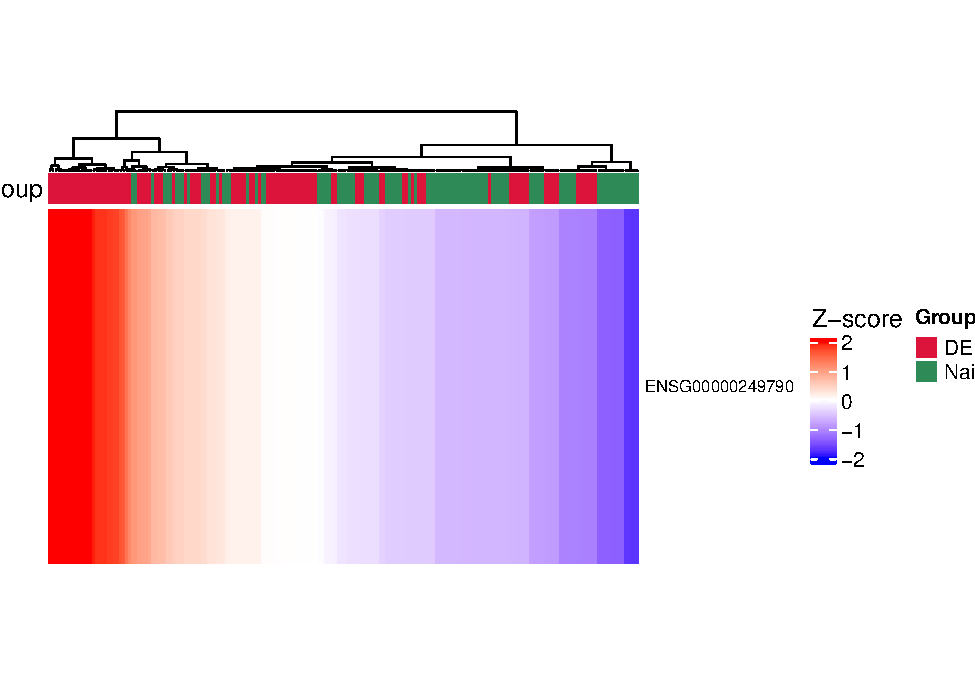
\includegraphics[keepaspectratio]{Assignment2_trimmed_files/figure-latex/unnamed-chunk-15-1.pdf}}

\begin{Shaded}
\begin{Highlighting}[]
\CommentTok{\# Save the list of genes used in the heatmap}
\NormalTok{heatmap\_genes\_df }\OtherTok{\textless{}{-}} \FunctionTok{data.frame}\NormalTok{(}
  \AttributeTok{GeneID =} \FunctionTok{rownames}\NormalTok{(scaled\_data),}
  \AttributeTok{GeneSymbol =}\NormalTok{ gene\_labels,}
  \AttributeTok{stringsAsFactors =} \ConstantTok{FALSE}
\NormalTok{)}

\ControlFlowTok{if}\NormalTok{ (}\FunctionTok{exists}\NormalTok{(}\StringTok{"res\_annot"}\NormalTok{)) \{}
\NormalTok{  heatmap\_genes\_df }\OtherTok{\textless{}{-}}\NormalTok{ heatmap\_genes\_df }\SpecialCharTok{\%\textgreater{}\%}
    \FunctionTok{left\_join}\NormalTok{(res\_annot }\SpecialCharTok{\%\textgreater{}\%} \FunctionTok{select}\NormalTok{(GeneID, log2FoldChange, padj), }\AttributeTok{by =} \StringTok{"GeneID"}\NormalTok{)}
\NormalTok{\} }\ControlFlowTok{else} \ControlFlowTok{if}\NormalTok{ (}\FunctionTok{exists}\NormalTok{(}\StringTok{"res\_df"}\NormalTok{)) \{}
\NormalTok{  heatmap\_genes\_df }\OtherTok{\textless{}{-}}\NormalTok{ heatmap\_genes\_df }\SpecialCharTok{\%\textgreater{}\%}
    \FunctionTok{left\_join}\NormalTok{(res\_df }\SpecialCharTok{\%\textgreater{}\%} \FunctionTok{select}\NormalTok{(GeneID, log2FoldChange, padj), }\AttributeTok{by =} \StringTok{"GeneID"}\NormalTok{)}
\NormalTok{\}}

\CommentTok{\# Save to results directory}
\ControlFlowTok{if}\NormalTok{ (}\SpecialCharTok{!}\FunctionTok{dir.exists}\NormalTok{(results\_dir)) \{}
  \FunctionTok{dir.create}\NormalTok{(results\_dir, }\AttributeTok{recursive =} \ConstantTok{TRUE}\NormalTok{)}
\NormalTok{\}}
\NormalTok{readr}\SpecialCharTok{::}\FunctionTok{write\_tsv}\NormalTok{(heatmap\_genes\_df, }\FunctionTok{file.path}\NormalTok{(results\_dir, }\StringTok{"heatmap\_genes\_list.tsv"}\NormalTok{))}

\FunctionTok{cat}\NormalTok{(}\StringTok{"}\SpecialCharTok{\textbackslash{}n}\StringTok{Heatmap Summary:}\SpecialCharTok{\textbackslash{}n}\StringTok{"}\NormalTok{)}
\end{Highlighting}
\end{Shaded}

\begin{verbatim}
## 
## Heatmap Summary:
\end{verbatim}

\begin{Shaded}
\begin{Highlighting}[]
\FunctionTok{cat}\NormalTok{(}\StringTok{"{-} Genes displayed:"}\NormalTok{, }\FunctionTok{nrow}\NormalTok{(scaled\_data), }\StringTok{"}\SpecialCharTok{\textbackslash{}n}\StringTok{"}\NormalTok{)}
\end{Highlighting}
\end{Shaded}

\begin{verbatim}
## - Genes displayed: 65
\end{verbatim}

\begin{Shaded}
\begin{Highlighting}[]
\FunctionTok{cat}\NormalTok{(}\StringTok{"{-} Samples displayed:"}\NormalTok{, }\FunctionTok{ncol}\NormalTok{(scaled\_data), }\StringTok{"}\SpecialCharTok{\textbackslash{}n}\StringTok{"}\NormalTok{)}
\end{Highlighting}
\end{Shaded}

\begin{verbatim}
## - Samples displayed: 250
\end{verbatim}

\begin{Shaded}
\begin{Highlighting}[]
\FunctionTok{cat}\NormalTok{(}\StringTok{"{-} Sample groups:"}\NormalTok{, }\FunctionTok{paste}\NormalTok{(}\FunctionTok{names}\NormalTok{(}\FunctionTok{table}\NormalTok{(sample\_groups)), }\AttributeTok{collapse =} \StringTok{", "}\NormalTok{), }\StringTok{"}\SpecialCharTok{\textbackslash{}n}\StringTok{"}\NormalTok{)}
\end{Highlighting}
\end{Shaded}

\begin{verbatim}
## - Sample groups: DENV, Naive
\end{verbatim}

\begin{Shaded}
\begin{Highlighting}[]
\FunctionTok{cat}\NormalTok{(}\StringTok{"{-} Data transformation: log2(normalized counts + 1), then z{-}score normalized by gene}\SpecialCharTok{\textbackslash{}n}\StringTok{"}\NormalTok{)}
\end{Highlighting}
\end{Shaded}

\begin{verbatim}
## - Data transformation: log2(normalized counts + 1), then z-score normalized by gene
\end{verbatim}

\begin{Shaded}
\begin{Highlighting}[]
\FunctionTok{cat}\NormalTok{(}\StringTok{"{-} Clustering: Hierarchical clustering with euclidean distance and complete linkage}\SpecialCharTok{\textbackslash{}n}\StringTok{"}\NormalTok{)}
\end{Highlighting}
\end{Shaded}

\begin{verbatim}
## - Clustering: Hierarchical clustering with euclidean distance and complete linkage
\end{verbatim}

\begin{Shaded}
\begin{Highlighting}[]
\FunctionTok{cat}\NormalTok{(}\StringTok{"{-} Files saved:"}\NormalTok{, heatmap\_file, }\StringTok{"and"}\NormalTok{, heatmap\_file\_pdf, }\StringTok{"}\SpecialCharTok{\textbackslash{}n}\StringTok{"}\NormalTok{)}
\end{Highlighting}
\end{Shaded}

\begin{verbatim}
## - Files saved: plots/heatmap_significant_genes.png and plots/heatmap_significant_genes.pdf
\end{verbatim}

\subsection{Section 4 Summary}\label{section-4-summary}

\begin{verbatim}
## The heatmap contrasts 65 high-confidence genes across 250 samples, revealing clear separation between the DENV: 141; Naive: 109 groups after z-score scaling of normalized counts. Sample annotations on the column sidebar reflect the Exposure2 labels used in the differential expression analysis, and both PNG and PDF versions are stored in the plots directory.
\end{verbatim}

\section{Section 5: William Le}\label{section-5-william-le}

GenomicSuperSignature \#\# Install

\begin{Shaded}
\begin{Highlighting}[]
\ControlFlowTok{if}\NormalTok{ (}\SpecialCharTok{!}\FunctionTok{requireNamespace}\NormalTok{(}\StringTok{"GenomicSuperSignature"}\NormalTok{, }\AttributeTok{quietly =} \ConstantTok{TRUE}\NormalTok{)) \{}
  \ControlFlowTok{if}\NormalTok{ (}\SpecialCharTok{!}\FunctionTok{requireNamespace}\NormalTok{(}\StringTok{"BiocManager"}\NormalTok{, }\AttributeTok{quietly =} \ConstantTok{TRUE}\NormalTok{)) }\FunctionTok{install.packages}\NormalTok{(}\StringTok{"BiocManager"}\NormalTok{, }\AttributeTok{repos =} \FunctionTok{getOption}\NormalTok{(}\StringTok{"repos"}\NormalTok{)[}\StringTok{"CRAN"}\NormalTok{])}
\NormalTok{  BiocManager}\SpecialCharTok{::}\FunctionTok{install}\NormalTok{(}\StringTok{"GenomicSuperSignature"}\NormalTok{, }\AttributeTok{ask =} \ConstantTok{FALSE}\NormalTok{, }\AttributeTok{update =} \ConstantTok{FALSE}\NormalTok{)}
\NormalTok{\}}
\ControlFlowTok{if}\NormalTok{ (}\SpecialCharTok{!}\FunctionTok{requireNamespace}\NormalTok{(}\StringTok{"bcellViper"}\NormalTok{, }\AttributeTok{quietly =} \ConstantTok{TRUE}\NormalTok{)) \{}
  \ControlFlowTok{if}\NormalTok{ (}\SpecialCharTok{!}\FunctionTok{requireNamespace}\NormalTok{(}\StringTok{"BiocManager"}\NormalTok{, }\AttributeTok{quietly =} \ConstantTok{TRUE}\NormalTok{)) }\FunctionTok{install.packages}\NormalTok{(}\StringTok{"BiocManager"}\NormalTok{, }\AttributeTok{repos =} \FunctionTok{getOption}\NormalTok{(}\StringTok{"repos"}\NormalTok{)[}\StringTok{"CRAN"}\NormalTok{])}
\NormalTok{  BiocManager}\SpecialCharTok{::}\FunctionTok{install}\NormalTok{(}\StringTok{"bcellViper"}\NormalTok{, }\AttributeTok{ask =} \ConstantTok{FALSE}\NormalTok{, }\AttributeTok{update =} \ConstantTok{FALSE}\NormalTok{)}
\NormalTok{\}}
\end{Highlighting}
\end{Shaded}

\subsection{Libraries}\label{libraries}

\begin{Shaded}
\begin{Highlighting}[]
\FunctionTok{library}\NormalTok{(GenomicSuperSignature)}
\FunctionTok{library}\NormalTok{(bcellViper)}
\CommentTok{\# load RAV}
\NormalTok{RAVmodel }\OtherTok{\textless{}{-}} \FunctionTok{getModel}\NormalTok{(}\StringTok{"PLIERpriors"}\NormalTok{, }\AttributeTok{load=}\ConstantTok{TRUE}\NormalTok{)}
\end{Highlighting}
\end{Shaded}

\subsection{Data Wrangle Ranked Gene
List}\label{data-wrangle-ranked-gene-list}

Validate expects a Expression Set or simple matrix.

\begin{Shaded}
\begin{Highlighting}[]
\CommentTok{\# Define the file path to the data directory}
\NormalTok{data\_dir }\OtherTok{\textless{}{-}} \FunctionTok{file.path}\NormalTok{(}\StringTok{"data"}\NormalTok{, }\StringTok{"SRP192714"}\NormalTok{)}

\CommentTok{\# Declare the file path to the gene expression matrix file}
\NormalTok{data\_file }\OtherTok{\textless{}{-}} \FunctionTok{file.path}\NormalTok{(data\_dir, }\StringTok{"SRP192714.tsv"}\NormalTok{)}

\CommentTok{\# Read in data TSV file}
\NormalTok{expression\_df }\OtherTok{\textless{}{-}}\NormalTok{ readr}\SpecialCharTok{::}\FunctionTok{read\_tsv}\NormalTok{(data\_file, }\AttributeTok{show\_col\_types =} \ConstantTok{FALSE}\NormalTok{)}

\CommentTok{\# Respect trimmed runs by subsetting to the current sample selection when available}
\ControlFlowTok{if}\NormalTok{ (}\FunctionTok{exists}\NormalTok{(}\StringTok{"selected\_samples"}\NormalTok{)) \{}
\NormalTok{  sample\_cols }\OtherTok{\textless{}{-}} \FunctionTok{intersect}\NormalTok{(selected\_samples, }\FunctionTok{colnames}\NormalTok{(expression\_df))}
  \ControlFlowTok{if}\NormalTok{ (}\FunctionTok{length}\NormalTok{(sample\_cols) }\SpecialCharTok{==} \DecValTok{0}\NormalTok{) \{}
    \FunctionTok{stop}\NormalTok{(}\StringTok{"No overlap between selected\_samples and expression matrix columns for GenomicSuperSignature chunk."}\NormalTok{)}
\NormalTok{  \}}
\NormalTok{  expression\_df }\OtherTok{\textless{}{-}}\NormalTok{ expression\_df }\SpecialCharTok{\%\textgreater{}\%}
\NormalTok{    dplyr}\SpecialCharTok{::}\FunctionTok{select}\NormalTok{(dplyr}\SpecialCharTok{::}\FunctionTok{any\_of}\NormalTok{(}\FunctionTok{c}\NormalTok{(}\StringTok{"Gene"}\NormalTok{, sample\_cols)))}
\NormalTok{\}}

\CommentTok{\# Ensemble to Gene Name}
\NormalTok{mapped\_list }\OtherTok{\textless{}{-}} \FunctionTok{mapIds}\NormalTok{(}
\NormalTok{  org.Hs.eg.db, }\CommentTok{\# Annotation package for humans}
  \AttributeTok{keys =}\NormalTok{ expression\_df}\SpecialCharTok{$}\NormalTok{Gene,}
  \AttributeTok{keytype =} \StringTok{"ENSEMBL"}\NormalTok{,}
  \AttributeTok{column =} \StringTok{"SYMBOL"}\NormalTok{)}
\end{Highlighting}
\end{Shaded}

\begin{verbatim}
## 'select()' returned 1:many mapping between keys and columns
\end{verbatim}

\begin{Shaded}
\begin{Highlighting}[]
\CommentTok{\# List to df}
\NormalTok{mapped\_df }\OtherTok{\textless{}{-}}\NormalTok{ mapped\_list }\SpecialCharTok{\%\textgreater{}\%}
\NormalTok{  tibble}\SpecialCharTok{::}\FunctionTok{enframe}\NormalTok{(}\AttributeTok{name =} \StringTok{"Ensembl"}\NormalTok{, }\AttributeTok{value =} \StringTok{"Gene"}\NormalTok{) }\SpecialCharTok{\%\textgreater{}\%}
  \CommentTok{\# This will result in one row of our data frame per list item}
\NormalTok{  tidyr}\SpecialCharTok{::}\FunctionTok{unnest}\NormalTok{(}\AttributeTok{cols =}\NormalTok{ Gene)}

\CommentTok{\# Join then remove Ensembl {-}{-} use conservative join syntax for compatibility}
\NormalTok{cts }\OtherTok{\textless{}{-}} \FunctionTok{tryCatch}\NormalTok{(}
\NormalTok{  \{}
\NormalTok{    mapped\_df }\SpecialCharTok{\%\textgreater{}\%}
\NormalTok{      dplyr}\SpecialCharTok{::}\FunctionTok{inner\_join}\NormalTok{(expression\_df, }\AttributeTok{by =} \FunctionTok{c}\NormalTok{(}\StringTok{"Ensembl"} \OtherTok{=} \StringTok{"Gene"}\NormalTok{)) }\SpecialCharTok{\%\textgreater{}\%}
\NormalTok{      dplyr}\SpecialCharTok{::}\FunctionTok{select}\NormalTok{(}\SpecialCharTok{{-}}\NormalTok{Ensembl)}
\NormalTok{  \}, }\AttributeTok{error =} \ControlFlowTok{function}\NormalTok{(e) \{}
    \CommentTok{\# fallback: if join fails, attempt a manual merge}
\NormalTok{    merged }\OtherTok{\textless{}{-}} \FunctionTok{merge}\NormalTok{(mapped\_df, expression\_df, }\AttributeTok{by.x =} \StringTok{"Ensembl"}\NormalTok{, }\AttributeTok{by.y =} \StringTok{"Gene"}\NormalTok{, }\AttributeTok{all.x =} \ConstantTok{FALSE}\NormalTok{, }\AttributeTok{all.y =} \ConstantTok{FALSE}\NormalTok{)}
\NormalTok{    tibble}\SpecialCharTok{::}\FunctionTok{as\_tibble}\NormalTok{(merged) }\SpecialCharTok{\%\textgreater{}\%}\NormalTok{ dplyr}\SpecialCharTok{::}\FunctionTok{select}\NormalTok{(}\SpecialCharTok{{-}}\NormalTok{Ensembl)}
\NormalTok{  \}}
\NormalTok{)}

\CommentTok{\# Filter for na}
\NormalTok{cts\_filtered }\OtherTok{\textless{}{-}}\NormalTok{ cts }\SpecialCharTok{\%\textgreater{}\%}
\NormalTok{  tidyr}\SpecialCharTok{::}\FunctionTok{drop\_na}\NormalTok{(Gene)}

\CommentTok{\# Drop low average count dupes}
\NormalTok{cts\_matrix }\OtherTok{\textless{}{-}}\NormalTok{ cts\_filtered }\SpecialCharTok{\%\textgreater{}\%}
\NormalTok{  dplyr}\SpecialCharTok{::}\FunctionTok{group\_by}\NormalTok{(Gene) }\SpecialCharTok{\%\textgreater{}\%}
\NormalTok{  dplyr}\SpecialCharTok{::}\FunctionTok{summarise}\NormalTok{(}\FunctionTok{across}\NormalTok{(}\FunctionTok{everything}\NormalTok{(), sum)) }\SpecialCharTok{\%\textgreater{}\%}
\NormalTok{  tibble}\SpecialCharTok{::}\FunctionTok{column\_to\_rownames}\NormalTok{(}\StringTok{"Gene"}\NormalTok{) }\SpecialCharTok{\%\textgreater{}\%}
  \FunctionTok{as.matrix}\NormalTok{()}

\CommentTok{\# Ensure columns retain trimmed ordering and align with metadata when present}
\ControlFlowTok{if}\NormalTok{ (}\FunctionTok{exists}\NormalTok{(}\StringTok{"selected\_samples"}\NormalTok{)) \{}
\NormalTok{  keep\_order }\OtherTok{\textless{}{-}} \FunctionTok{intersect}\NormalTok{(selected\_samples, }\FunctionTok{colnames}\NormalTok{(cts\_matrix))}
  \ControlFlowTok{if}\NormalTok{ (}\FunctionTok{length}\NormalTok{(keep\_order) }\SpecialCharTok{\textgreater{}} \DecValTok{0}\NormalTok{) \{}
\NormalTok{    cts\_matrix }\OtherTok{\textless{}{-}}\NormalTok{ cts\_matrix[, keep\_order, drop }\OtherTok{=} \ConstantTok{FALSE}\NormalTok{]}
\NormalTok{  \}}
\NormalTok{\}}
\ControlFlowTok{if}\NormalTok{ (}\FunctionTok{exists}\NormalTok{(}\StringTok{"metadata"}\NormalTok{)) \{}
\NormalTok{  meta\_order }\OtherTok{\textless{}{-}} \FunctionTok{intersect}\NormalTok{(metadata}\SpecialCharTok{$}\NormalTok{refinebio\_accession\_code, }\FunctionTok{colnames}\NormalTok{(cts\_matrix))}
  \ControlFlowTok{if}\NormalTok{ (}\FunctionTok{length}\NormalTok{(meta\_order) }\SpecialCharTok{\textgreater{}} \DecValTok{0}\NormalTok{) \{}
\NormalTok{    cts\_matrix }\OtherTok{\textless{}{-}}\NormalTok{ cts\_matrix[, meta\_order, drop }\OtherTok{=} \ConstantTok{FALSE}\NormalTok{]}
\NormalTok{  \}}
\NormalTok{\}}

\CommentTok{\# Check if this is in the same order}
\FunctionTok{all.equal}\NormalTok{(}\FunctionTok{colnames}\NormalTok{(cts\_matrix), metadata}\SpecialCharTok{$}\NormalTok{refinebio\_accession\_code)}
\end{Highlighting}
\end{Shaded}

\begin{verbatim}
## [1] TRUE
\end{verbatim}

\begin{Shaded}
\begin{Highlighting}[]
\CommentTok{\# Validate on RAV}
\NormalTok{validated\_list }\OtherTok{\textless{}{-}}\NormalTok{ GenomicSuperSignature}\SpecialCharTok{::}\FunctionTok{validate}\NormalTok{(cts\_matrix, RAVmodel)}
\FunctionTok{head}\NormalTok{(validated\_list)}
\end{Highlighting}
\end{Shaded}

\begin{verbatim}
##           score PC          sw cl_size cl_num
## RAV1 0.05876213  1 -0.05470163       6      1
## RAV2 0.08662300  3  0.06426256      21      2
## RAV3 0.12923861  3 -0.01800335       4      3
## RAV4 0.26329091  1 -0.04005584       7      4
## RAV5 0.16073616  1  0.05786189       3      5
## RAV6 0.13187769  1 -0.02520973       3      6
\end{verbatim}

\begin{Shaded}
\begin{Highlighting}[]
\NormalTok{validated\_ind }\OtherTok{\textless{}{-}} \FunctionTok{validatedSignatures}\NormalTok{(validated\_list, RAVmodel, }\AttributeTok{num.out =} \DecValTok{3}\NormalTok{, }
                                     \AttributeTok{swCutoff =} \DecValTok{0}\NormalTok{, }\AttributeTok{indexOnly =} \ConstantTok{TRUE}\NormalTok{)}
\end{Highlighting}
\end{Shaded}

\subsection{Tables}\label{tables}

\begin{Shaded}
\begin{Highlighting}[]
\FunctionTok{annotateRAV}\NormalTok{(RAVmodel, validated\_ind[}\DecValTok{3}\NormalTok{])}
\end{Highlighting}
\end{Shaded}

\begin{verbatim}
##               Description      NES pvalue      qvalues
## 1 IRIS_Neutrophil-Resting 4.242584  1e-10 1.803828e-09
## 2      IRIS_Monocyte-Day0 3.420260  1e-10 1.803828e-09
## 3         SVM Neutrophils 3.328093  1e-10 1.803828e-09
## 4              DMAP_MONO2 3.173188  1e-10 1.803828e-09
## 5           SVM Monocytes 3.116177  1e-10 1.803828e-09
\end{verbatim}

\begin{Shaded}
\begin{Highlighting}[]
\FunctionTok{heatmapTable}\NormalTok{(validated\_list, RAVmodel)}
\end{Highlighting}
\end{Shaded}

\pandocbounded{\includegraphics[keepaspectratio]{Assignment2_trimmed_files/figure-latex/GSEA-1.pdf}}

\begin{Shaded}
\begin{Highlighting}[]
\FunctionTok{meshTable}\NormalTok{(RAVmodel, validated\_ind[}\DecValTok{2}\NormalTok{])}
\end{Highlighting}
\end{Shaded}

\begin{verbatim}
##                                     word         freq
## 19                   Malaria, Falciparum 0.0348621676
## 22                 Plasmodium falciparum 0.0278897341
## 18                               Malaria 0.0232414451
## 21                             Parasites 0.0199212386
## 15                Innate Immune Response 0.0174310838
## 10                     Genetic Variation 0.0126771519
## 3                            Amino Acids 0.0091398605
## 17                   Latent Tuberculosis 0.0082035351
## 37                              Vaccines 0.0076381114
## 20                            Metabolome 0.0073118884
## 11                              Genotype 0.0069724335
## 8                                  Donor 0.0068768253
## 23                   Prospective Studies 0.0063805273
## 14                             Incidence 0.0057424746
## 16                                Kidney 0.0045699302
## 25                             Pyridones 0.0045699302
## 31                       Systems Biology 0.0040621602
## 34                          Tuberculosis 0.0035890466
## 35                        United Kingdom 0.0035478731
## 2                              Algorithm 0.0030552446
## 36                           Vaccination 0.0030552446
## 30                              Software 0.0021823175
## 24                              Proteome 0.0021505554
## 28                  Rheumatoid Arthritis 0.0021159462
## 33                Transcriptome Analysis 0.0021128586
## 7                         Cohort Studies 0.0008834576
## 6                             Biomarkers 0.0008444816
## 1                                  Adult 0.0008040117
## 12 High-Throughput Nucleotide Sequencing 0.0007767571
## 9                           Gene Library 0.0007638111
## 4                                Animals 0.0006672185
## 26                                   RNA 0.0005963354
## 32                         Transcriptome 0.0003533254
## 27                               RNA-Seq 0.0003134980
## 5                          Base Sequence 0.0003054508
## 13                                Humans 0.0002637737
## 29                       Sequencing, RNA 0.0002073096
## 38                                  mRNA 0.0001766157
\end{verbatim}

\begin{verbatim}
## Wrote GenomicSuperSignature summary to: results/GSS_validated_signatures_trimmed_250.tsv
\end{verbatim}

\section{Section 5: Nikhil Sangamkar}\label{section-5-nikhil-sangamkar}

\begin{Shaded}
\begin{Highlighting}[]
\ControlFlowTok{if}\NormalTok{ (}\SpecialCharTok{!}\FunctionTok{requireNamespace}\NormalTok{(}\StringTok{"clusterProfiler"}\NormalTok{, }\AttributeTok{quietly =} \ConstantTok{TRUE}\NormalTok{)) \{}
\NormalTok{  BiocManager}\SpecialCharTok{::}\FunctionTok{install}\NormalTok{(}\StringTok{"clusterProfiler"}\NormalTok{, }\AttributeTok{ask =} \ConstantTok{FALSE}\NormalTok{, }\AttributeTok{update =} \ConstantTok{FALSE}\NormalTok{)}
\NormalTok{\}}
\end{Highlighting}
\end{Shaded}

\begin{verbatim}
## 
\end{verbatim}

\begin{Shaded}
\begin{Highlighting}[]
\ControlFlowTok{if}\NormalTok{ (}\SpecialCharTok{!}\FunctionTok{requireNamespace}\NormalTok{(}\StringTok{"org.Hs.eg.db"}\NormalTok{, }\AttributeTok{quietly =} \ConstantTok{TRUE}\NormalTok{)) \{}
\NormalTok{  BiocManager}\SpecialCharTok{::}\FunctionTok{install}\NormalTok{(}\StringTok{"org.Hs.eg.db"}\NormalTok{, }\AttributeTok{ask =} \ConstantTok{FALSE}\NormalTok{, }\AttributeTok{update =} \ConstantTok{FALSE}\NormalTok{)}
\NormalTok{\}}
\ControlFlowTok{if}\NormalTok{ (}\SpecialCharTok{!}\FunctionTok{requireNamespace}\NormalTok{(}\StringTok{"enrichplot"}\NormalTok{, }\AttributeTok{quietly =} \ConstantTok{TRUE}\NormalTok{)) \{}
\NormalTok{  BiocManager}\SpecialCharTok{::}\FunctionTok{install}\NormalTok{(}\StringTok{"enrichplot"}\NormalTok{, }\AttributeTok{ask =} \ConstantTok{FALSE}\NormalTok{, }\AttributeTok{update =} \ConstantTok{FALSE}\NormalTok{)}
\NormalTok{\}}

\FunctionTok{suppressPackageStartupMessages}\NormalTok{(\{}
  \FunctionTok{library}\NormalTok{(clusterProfiler)}
  \FunctionTok{library}\NormalTok{(org.Hs.eg.db)}
  \FunctionTok{library}\NormalTok{(enrichplot)}
  \FunctionTok{library}\NormalTok{(dplyr)}
  \FunctionTok{library}\NormalTok{(readr)}
  \FunctionTok{library}\NormalTok{(ggplot2)}
\NormalTok{\})}

\FunctionTok{stopifnot}\NormalTok{(}\FunctionTok{exists}\NormalTok{(}\StringTok{"res\_df"}\NormalTok{), }\FunctionTok{exists}\NormalTok{(}\StringTok{"results\_dir"}\NormalTok{), }\FunctionTok{exists}\NormalTok{(}\StringTok{"plots\_dir"}\NormalTok{))}

\NormalTok{sig\_genes\_all }\OtherTok{\textless{}{-}}\NormalTok{ res\_df }\SpecialCharTok{\%\textgreater{}\%}
  \FunctionTok{filter}\NormalTok{(}\SpecialCharTok{!}\FunctionTok{is.na}\NormalTok{(padj) }\SpecialCharTok{\&}\NormalTok{ padj }\SpecialCharTok{\textless{}} \FloatTok{0.05}\NormalTok{) }\SpecialCharTok{\%\textgreater{}\%}
  \FunctionTok{pull}\NormalTok{(GeneID)}

\ControlFlowTok{if}\NormalTok{ (}\FunctionTok{length}\NormalTok{(sig\_genes\_all) }\SpecialCharTok{\textless{}} \DecValTok{5}\NormalTok{) \{}
  \FunctionTok{warning}\NormalTok{(}\StringTok{"Fewer than five significant genes available; skipping KEGG enrichment."}\NormalTok{)}
\NormalTok{\} }\ControlFlowTok{else}\NormalTok{ \{}
\NormalTok{  clean\_ids }\OtherTok{\textless{}{-}} \FunctionTok{gsub}\NormalTok{(}\StringTok{"}\SpecialCharTok{\textbackslash{}\textbackslash{}}\StringTok{.}\SpecialCharTok{\textbackslash{}\textbackslash{}}\StringTok{d+$"}\NormalTok{, }\StringTok{""}\NormalTok{, sig\_genes\_all)}
\NormalTok{  entrez\_map }\OtherTok{\textless{}{-}} \FunctionTok{bitr}\NormalTok{(}\FunctionTok{unique}\NormalTok{(clean\_ids),}
                     \AttributeTok{fromType =} \StringTok{"ENSEMBL"}\NormalTok{,}
                     \AttributeTok{toType =} \StringTok{"ENTREZID"}\NormalTok{,}
                     \AttributeTok{OrgDb =}\NormalTok{ org.Hs.eg.db,}
                     \AttributeTok{drop =} \ConstantTok{TRUE}\NormalTok{)}
\NormalTok{  entrez\_ids }\OtherTok{\textless{}{-}} \FunctionTok{unique}\NormalTok{(entrez\_map}\SpecialCharTok{$}\NormalTok{ENTREZID)}

  \ControlFlowTok{if}\NormalTok{ (}\FunctionTok{length}\NormalTok{(entrez\_ids) }\SpecialCharTok{\textless{}} \DecValTok{5}\NormalTok{) \{}
    \FunctionTok{warning}\NormalTok{(}\StringTok{"Not enough Entrez IDs mapped for KEGG enrichment."}\NormalTok{)}
\NormalTok{  \} }\ControlFlowTok{else}\NormalTok{ \{}
\NormalTok{    kegg\_enrich }\OtherTok{\textless{}{-}} \FunctionTok{suppressWarnings}\NormalTok{(}
      \FunctionTok{enrichKEGG}\NormalTok{(}
        \AttributeTok{gene =}\NormalTok{ entrez\_ids,}
        \AttributeTok{organism =} \StringTok{"hsa"}\NormalTok{,}
        \AttributeTok{keyType =} \StringTok{"ncbi{-}geneid"}\NormalTok{,}
        \AttributeTok{pvalueCutoff =} \FloatTok{0.05}\NormalTok{,}
        \AttributeTok{qvalueCutoff =} \FloatTok{0.2}
\NormalTok{      )}
\NormalTok{    )}

    \ControlFlowTok{if}\NormalTok{ (}\FunctionTok{is.null}\NormalTok{(kegg\_enrich) }\SpecialCharTok{||} \FunctionTok{nrow}\NormalTok{(}\FunctionTok{as.data.frame}\NormalTok{(kegg\_enrich)) }\SpecialCharTok{==} \DecValTok{0}\NormalTok{) \{}
      \FunctionTok{message}\NormalTok{(}\StringTok{"No significant KEGG pathways detected for the chosen threshold."}\NormalTok{)}
\NormalTok{    \} }\ControlFlowTok{else}\NormalTok{ \{}
\NormalTok{      kegg\_enrich }\OtherTok{\textless{}{-}} \FunctionTok{setReadable}\NormalTok{(kegg\_enrich, }\AttributeTok{OrgDb =}\NormalTok{ org.Hs.eg.db, }\AttributeTok{keyType =} \StringTok{"ENTREZID"}\NormalTok{)}
\NormalTok{      kegg\_df }\OtherTok{\textless{}{-}} \FunctionTok{as.data.frame}\NormalTok{(kegg\_enrich)}

      \ControlFlowTok{if}\NormalTok{ (}\SpecialCharTok{!}\FunctionTok{dir.exists}\NormalTok{(results\_dir)) }\FunctionTok{dir.create}\NormalTok{(results\_dir, }\AttributeTok{recursive =} \ConstantTok{TRUE}\NormalTok{)}
      \ControlFlowTok{if}\NormalTok{ (}\SpecialCharTok{!}\FunctionTok{dir.exists}\NormalTok{(plots\_dir)) }\FunctionTok{dir.create}\NormalTok{(plots\_dir, }\AttributeTok{recursive =} \ConstantTok{TRUE}\NormalTok{)}

\NormalTok{      kegg\_path }\OtherTok{\textless{}{-}} \FunctionTok{file.path}\NormalTok{(results\_dir, }\FunctionTok{paste0}\NormalTok{(}\StringTok{"KEGG\_enrichment\_"}\NormalTok{, run\_label, }\StringTok{".tsv"}\NormalTok{))}
\NormalTok{      readr}\SpecialCharTok{::}\FunctionTok{write\_tsv}\NormalTok{(kegg\_df, kegg\_path)}

\NormalTok{      top\_kegg }\OtherTok{\textless{}{-}}\NormalTok{ kegg\_df }\SpecialCharTok{\%\textgreater{}\%} \FunctionTok{slice\_head}\NormalTok{(}\AttributeTok{n =} \DecValTok{20}\NormalTok{)}
\NormalTok{      readr}\SpecialCharTok{::}\FunctionTok{write\_tsv}\NormalTok{(top\_kegg, }\FunctionTok{file.path}\NormalTok{(results\_dir, }\FunctionTok{paste0}\NormalTok{(}\StringTok{"KEGG\_enrichment\_top20\_"}\NormalTok{, run\_label, }\StringTok{".tsv"}\NormalTok{)))}

\NormalTok{      kegg\_dot }\OtherTok{\textless{}{-}} \FunctionTok{dotplot}\NormalTok{(kegg\_enrich, }\AttributeTok{showCategory =} \FunctionTok{min}\NormalTok{(}\DecValTok{15}\NormalTok{, }\FunctionTok{nrow}\NormalTok{(kegg\_df))) }\SpecialCharTok{+}
        \FunctionTok{labs}\NormalTok{(}\AttributeTok{title =} \StringTok{"KEGG Pathway Enrichment"}\NormalTok{, }\AttributeTok{subtitle =} \FunctionTok{paste0}\NormalTok{(}\StringTok{"Nikhil Sangamkar ("}\NormalTok{, run\_label, }\StringTok{")"}\NormalTok{)) }\SpecialCharTok{+}
        \FunctionTok{theme}\NormalTok{(}\AttributeTok{axis.text.y =} \FunctionTok{element\_text}\NormalTok{(}\AttributeTok{size =} \DecValTok{8}\NormalTok{))}
      \FunctionTok{ggsave}\NormalTok{(}\FunctionTok{file.path}\NormalTok{(plots\_dir, }\FunctionTok{paste0}\NormalTok{(}\StringTok{"KEGG\_enrichment\_dotplot\_"}\NormalTok{, run\_label, }\StringTok{".png"}\NormalTok{)),}
\NormalTok{             kegg\_dot, }\AttributeTok{width =} \DecValTok{10}\NormalTok{, }\AttributeTok{height =} \DecValTok{7}\NormalTok{, }\AttributeTok{dpi =} \DecValTok{300}\NormalTok{)}

      \FunctionTok{assign}\NormalTok{(}\StringTok{"kegg\_results\_df"}\NormalTok{, kegg\_df, }\AttributeTok{envir =}\NormalTok{ .GlobalEnv)}
\NormalTok{    \}}
\NormalTok{  \}}
\NormalTok{\}}
\end{Highlighting}
\end{Shaded}

\begin{verbatim}
## 'select()' returned 1:1 mapping between keys and columns
\end{verbatim}

\begin{verbatim}
## Warning in bitr(unique(clean_ids), fromType = "ENSEMBL", toType = "ENTREZID", :
## 3.08% of input gene IDs are fail to map...
\end{verbatim}

\begin{verbatim}
## Reading KEGG annotation online: "https://rest.kegg.jp/link/hsa/pathway"...
\end{verbatim}

\begin{verbatim}
## Reading KEGG annotation online: "https://rest.kegg.jp/list/pathway/hsa"...
\end{verbatim}

\begin{verbatim}
## Reading KEGG annotation online: "https://rest.kegg.jp/conv/ncbi-geneid/hsa"...
\end{verbatim}

\section{Section 5: Taylor Tillander}\label{section-5-taylor-tillander}

\begin{Shaded}
\begin{Highlighting}[]
\ControlFlowTok{if}\NormalTok{ (}\SpecialCharTok{!}\FunctionTok{requireNamespace}\NormalTok{(}\StringTok{"topGO"}\NormalTok{, }\AttributeTok{quietly =} \ConstantTok{TRUE}\NormalTok{)) \{}
\NormalTok{  BiocManager}\SpecialCharTok{::}\FunctionTok{install}\NormalTok{(}\StringTok{"topGO"}\NormalTok{, }\AttributeTok{ask =} \ConstantTok{FALSE}\NormalTok{, }\AttributeTok{update =} \ConstantTok{FALSE}\NormalTok{)}
\NormalTok{\}}
\ControlFlowTok{if}\NormalTok{ (}\SpecialCharTok{!}\FunctionTok{requireNamespace}\NormalTok{(}\StringTok{"GO.db"}\NormalTok{, }\AttributeTok{quietly =} \ConstantTok{TRUE}\NormalTok{)) \{}
\NormalTok{  BiocManager}\SpecialCharTok{::}\FunctionTok{install}\NormalTok{(}\StringTok{"GO.db"}\NormalTok{, }\AttributeTok{ask =} \ConstantTok{FALSE}\NormalTok{, }\AttributeTok{update =} \ConstantTok{FALSE}\NormalTok{)}
\NormalTok{\}}

\FunctionTok{suppressPackageStartupMessages}\NormalTok{(\{}
  \FunctionTok{library}\NormalTok{(topGO)}
  \FunctionTok{library}\NormalTok{(org.Hs.eg.db)}
  \FunctionTok{library}\NormalTok{(dplyr)}
  \FunctionTok{library}\NormalTok{(readr)}
  \FunctionTok{library}\NormalTok{(stringr)}
  \FunctionTok{library}\NormalTok{(ggplot2)}
\NormalTok{\})}
\end{Highlighting}
\end{Shaded}

\begin{verbatim}
## 
## groupGOTerms:    GOBPTerm, GOMFTerm, GOCCTerm environments built.
\end{verbatim}

\begin{Shaded}
\begin{Highlighting}[]
\FunctionTok{stopifnot}\NormalTok{(}\FunctionTok{exists}\NormalTok{(}\StringTok{"res\_df"}\NormalTok{))}

\CommentTok{\# prepare gene universe with one padj per Ensembl ID (version{-}stripped)}
\NormalTok{gene\_table }\OtherTok{\textless{}{-}}\NormalTok{ res\_df }\SpecialCharTok{\%\textgreater{}\%}
  \FunctionTok{transmute}\NormalTok{(}
    \AttributeTok{base\_id =} \FunctionTok{str\_remove}\NormalTok{(GeneID, }\StringTok{"}\SpecialCharTok{\textbackslash{}\textbackslash{}}\StringTok{.}\SpecialCharTok{\textbackslash{}\textbackslash{}}\StringTok{d+$"}\NormalTok{),}
    \AttributeTok{padj =}\NormalTok{ dplyr}\SpecialCharTok{::}\FunctionTok{coalesce}\NormalTok{(padj, }\DecValTok{1}\NormalTok{)}
\NormalTok{  ) }\SpecialCharTok{\%\textgreater{}\%}
  \FunctionTok{group\_by}\NormalTok{(base\_id) }\SpecialCharTok{\%\textgreater{}\%}
  \FunctionTok{summarize}\NormalTok{(}\AttributeTok{padj =} \FunctionTok{min}\NormalTok{(padj), }\AttributeTok{.groups =} \StringTok{"drop"}\NormalTok{)}

\NormalTok{gene\_scores }\OtherTok{\textless{}{-}}\NormalTok{ gene\_table}\SpecialCharTok{$}\NormalTok{padj}
\FunctionTok{names}\NormalTok{(gene\_scores) }\OtherTok{\textless{}{-}}\NormalTok{ gene\_table}\SpecialCharTok{$}\NormalTok{base\_id}

\NormalTok{selection\_fun }\OtherTok{\textless{}{-}} \ControlFlowTok{function}\NormalTok{(x) x }\SpecialCharTok{\textless{}} \FloatTok{0.05}

\NormalTok{go\_data\_bp }\OtherTok{\textless{}{-}}\NormalTok{ methods}\SpecialCharTok{::}\FunctionTok{new}\NormalTok{(}
  \StringTok{"topGOdata"}\NormalTok{,}
  \AttributeTok{description =} \StringTok{"topGO GO BP"}\NormalTok{,}
  \AttributeTok{ontology =} \StringTok{"BP"}\NormalTok{,}
  \AttributeTok{allGenes =}\NormalTok{ gene\_scores,}
  \AttributeTok{geneSel =}\NormalTok{ selection\_fun,}
  \AttributeTok{nodeSize =} \DecValTok{10}\NormalTok{,}
  \AttributeTok{annot =}\NormalTok{ annFUN.org,}
  \AttributeTok{mapping =} \StringTok{"org.Hs.eg.db"}\NormalTok{,}
  \AttributeTok{ID =} \StringTok{"ENSEMBL"}
\NormalTok{)}
\end{Highlighting}
\end{Shaded}

\begin{verbatim}
## 
## Building most specific GOs .....
\end{verbatim}

\begin{verbatim}
##  ( 11983 GO terms found. )
\end{verbatim}

\begin{verbatim}
## 
## Build GO DAG topology ..........
\end{verbatim}

\begin{verbatim}
##  ( 15025 GO terms and 33214 relations. )
\end{verbatim}

\begin{verbatim}
## 
## Annotating nodes ...............
\end{verbatim}

\begin{verbatim}
##  ( 16620 genes annotated to the GO terms. )
\end{verbatim}

\begin{Shaded}
\begin{Highlighting}[]
\NormalTok{result\_classic }\OtherTok{\textless{}{-}}\NormalTok{ topGO}\SpecialCharTok{::}\FunctionTok{runTest}\NormalTok{(go\_data\_bp, }\AttributeTok{algorithm =} \StringTok{"classic"}\NormalTok{, }\AttributeTok{statistic =} \StringTok{"fisher"}\NormalTok{)}
\end{Highlighting}
\end{Shaded}

\begin{verbatim}
## 
##           -- Classic Algorithm -- 
## 
##       the algorithm is scoring 2062 nontrivial nodes
##       parameters: 
##           test statistic: fisher
\end{verbatim}

\begin{Shaded}
\begin{Highlighting}[]
\NormalTok{result\_weight01 }\OtherTok{\textless{}{-}}\NormalTok{ topGO}\SpecialCharTok{::}\FunctionTok{runTest}\NormalTok{(go\_data\_bp, }\AttributeTok{algorithm =} \StringTok{"weight01"}\NormalTok{, }\AttributeTok{statistic =} \StringTok{"fisher"}\NormalTok{)}
\end{Highlighting}
\end{Shaded}

\begin{verbatim}
## 
##           -- Weight01 Algorithm -- 
## 
##       the algorithm is scoring 2062 nontrivial nodes
##       parameters: 
##           test statistic: fisher
\end{verbatim}

\begin{verbatim}
## 
##   Level 19:  1 nodes to be scored    (0 eliminated genes)
\end{verbatim}

\begin{verbatim}
## 
##   Level 18:  1 nodes to be scored    (0 eliminated genes)
\end{verbatim}

\begin{verbatim}
## 
##   Level 17:  4 nodes to be scored    (26 eliminated genes)
\end{verbatim}

\begin{verbatim}
## 
##   Level 16:  6 nodes to be scored    (42 eliminated genes)
\end{verbatim}

\begin{verbatim}
## 
##   Level 15:  11 nodes to be scored   (64 eliminated genes)
\end{verbatim}

\begin{verbatim}
## 
##   Level 14:  14 nodes to be scored   (126 eliminated genes)
\end{verbatim}

\begin{verbatim}
## 
##   Level 13:  22 nodes to be scored   (328 eliminated genes)
\end{verbatim}

\begin{verbatim}
## 
##   Level 12:  48 nodes to be scored   (640 eliminated genes)
\end{verbatim}

\begin{verbatim}
## 
##   Level 11:  105 nodes to be scored  (1647 eliminated genes)
\end{verbatim}

\begin{verbatim}
## 
##   Level 10:  179 nodes to be scored  (3897 eliminated genes)
\end{verbatim}

\begin{verbatim}
## 
##   Level 9:   237 nodes to be scored  (6310 eliminated genes)
\end{verbatim}

\begin{verbatim}
## 
##   Level 8:   305 nodes to be scored  (8494 eliminated genes)
\end{verbatim}

\begin{verbatim}
## 
##   Level 7:   329 nodes to be scored  (10667 eliminated genes)
\end{verbatim}

\begin{verbatim}
## 
##   Level 6:   328 nodes to be scored  (12527 eliminated genes)
\end{verbatim}

\begin{verbatim}
## 
##   Level 5:   242 nodes to be scored  (13901 eliminated genes)
\end{verbatim}

\begin{verbatim}
## 
##   Level 4:   148 nodes to be scored  (15561 eliminated genes)
\end{verbatim}

\begin{verbatim}
## 
##   Level 3:   66 nodes to be scored   (16154 eliminated genes)
\end{verbatim}

\begin{verbatim}
## 
##   Level 2:   15 nodes to be scored   (16493 eliminated genes)
\end{verbatim}

\begin{verbatim}
## 
##   Level 1:   1 nodes to be scored    (16568 eliminated genes)
\end{verbatim}

\begin{Shaded}
\begin{Highlighting}[]
\NormalTok{parse\_topgo\_p }\OtherTok{\textless{}{-}} \ControlFlowTok{function}\NormalTok{(x) \{}
\NormalTok{  vals }\OtherTok{\textless{}{-}}\NormalTok{ stringr}\SpecialCharTok{::}\FunctionTok{str\_trim}\NormalTok{(}\FunctionTok{as.character}\NormalTok{(x))}
\NormalTok{  vals }\OtherTok{\textless{}{-}}\NormalTok{ stringr}\SpecialCharTok{::}\FunctionTok{str\_replace\_all}\NormalTok{(vals, }\StringTok{"\textless{}"}\NormalTok{, }\StringTok{""}\NormalTok{)}
\NormalTok{  vals }\OtherTok{\textless{}{-}}\NormalTok{ stringr}\SpecialCharTok{::}\FunctionTok{str\_replace\_all}\NormalTok{(vals, }\StringTok{" "}\NormalTok{, }\StringTok{""}\NormalTok{)}
\NormalTok{  num }\OtherTok{\textless{}{-}} \FunctionTok{suppressWarnings}\NormalTok{(}\FunctionTok{as.numeric}\NormalTok{(vals))}
  \FunctionTok{ifelse}\NormalTok{(}\FunctionTok{is.na}\NormalTok{(num), }\DecValTok{1}\NormalTok{, num)}
\NormalTok{\}}

\NormalTok{go\_table\_bp }\OtherTok{\textless{}{-}}\NormalTok{ topGO}\SpecialCharTok{::}\FunctionTok{GenTable}\NormalTok{(}
\NormalTok{  go\_data\_bp,}
  \AttributeTok{classicFisher =}\NormalTok{ result\_classic,}
  \AttributeTok{weight01Fisher =}\NormalTok{ result\_weight01,}
  \AttributeTok{orderBy =} \StringTok{"weight01Fisher"}\NormalTok{,}
  \AttributeTok{topNodes =} \DecValTok{200}
\NormalTok{) }\SpecialCharTok{\%\textgreater{}\%}
  \FunctionTok{as\_tibble}\NormalTok{() }\SpecialCharTok{\%\textgreater{}\%}
  \FunctionTok{mutate}\NormalTok{(}
    \AttributeTok{classicFisher\_p =} \FunctionTok{parse\_topgo\_p}\NormalTok{(classicFisher),}
    \AttributeTok{weight01Fisher\_p =} \FunctionTok{parse\_topgo\_p}\NormalTok{(weight01Fisher),}
    \AttributeTok{neglog\_weight01 =} \SpecialCharTok{{-}}\FunctionTok{log10}\NormalTok{(weight01Fisher\_p)}
\NormalTok{  )}

\FunctionTok{assign}\NormalTok{(}\StringTok{"topgo\_results\_bp"}\NormalTok{, go\_table\_bp, }\AttributeTok{envir =}\NormalTok{ .GlobalEnv)}

\ControlFlowTok{if}\NormalTok{ (}\SpecialCharTok{!}\FunctionTok{dir.exists}\NormalTok{(results\_dir)) }\FunctionTok{dir.create}\NormalTok{(results\_dir, }\AttributeTok{recursive =} \ConstantTok{TRUE}\NormalTok{)}
\NormalTok{readr}\SpecialCharTok{::}\FunctionTok{write\_tsv}\NormalTok{(go\_table\_bp, }\FunctionTok{file.path}\NormalTok{(results\_dir, }\StringTok{"topGO\_BP.tsv"}\NormalTok{))}

\NormalTok{topgo\_top10 }\OtherTok{\textless{}{-}}\NormalTok{ go\_table\_bp }\SpecialCharTok{\%\textgreater{}\%} \FunctionTok{slice\_head}\NormalTok{(}\AttributeTok{n =} \DecValTok{10}\NormalTok{)}
\FunctionTok{assign}\NormalTok{(}\StringTok{"topgo\_top10\_bp"}\NormalTok{, topgo\_top10, }\AttributeTok{envir =}\NormalTok{ .GlobalEnv)}
\NormalTok{readr}\SpecialCharTok{::}\FunctionTok{write\_tsv}\NormalTok{(topgo\_top10, }\FunctionTok{file.path}\NormalTok{(results\_dir, }\StringTok{"topGO\_BP\_top10.tsv"}\NormalTok{))}

\ControlFlowTok{if}\NormalTok{ (}\SpecialCharTok{!}\FunctionTok{dir.exists}\NormalTok{(plots\_dir)) }\FunctionTok{dir.create}\NormalTok{(plots\_dir, }\AttributeTok{recursive =} \ConstantTok{TRUE}\NormalTok{)}
\NormalTok{topgo\_plot }\OtherTok{\textless{}{-}}\NormalTok{ topgo\_top10 }\SpecialCharTok{\%\textgreater{}\%}
  \FunctionTok{mutate}\NormalTok{(}\AttributeTok{Term =} \FunctionTok{factor}\NormalTok{(Term, }\AttributeTok{levels =} \FunctionTok{rev}\NormalTok{(Term[}\FunctionTok{order}\NormalTok{(neglog\_weight01)]))) }\SpecialCharTok{\%\textgreater{}\%}
  \FunctionTok{ggplot}\NormalTok{(}\FunctionTok{aes}\NormalTok{(neglog\_weight01, Term)) }\SpecialCharTok{+}
  \FunctionTok{geom\_col}\NormalTok{(}\AttributeTok{fill =} \StringTok{"\#3B82F6"}\NormalTok{) }\SpecialCharTok{+}
  \FunctionTok{labs}\NormalTok{(}
    \AttributeTok{title =} \StringTok{"topGO BP enrichment (weight01 Fisher)"}\NormalTok{,}
    \AttributeTok{x =} \StringTok{"{-}log10(weight01 Fisher p{-}value)"}\NormalTok{,}
    \AttributeTok{y =} \ConstantTok{NULL}
\NormalTok{  ) }\SpecialCharTok{+}
  \FunctionTok{theme\_minimal}\NormalTok{()}

\NormalTok{plot\_path }\OtherTok{\textless{}{-}} \FunctionTok{file.path}\NormalTok{(plots\_dir, }\FunctionTok{paste0}\NormalTok{(run\_label, }\StringTok{"\_topgo\_BP.png"}\NormalTok{))}
\FunctionTok{ggsave}\NormalTok{(plot\_path, topgo\_plot, }\AttributeTok{width =} \DecValTok{8}\NormalTok{, }\AttributeTok{height =} \DecValTok{5}\NormalTok{, }\AttributeTok{dpi =} \DecValTok{300}\NormalTok{)}
\NormalTok{topgo\_plot}
\end{Highlighting}
\end{Shaded}

\pandocbounded{\includegraphics[keepaspectratio]{Assignment2_trimmed_files/figure-latex/unnamed-chunk-20-1.pdf}}

\begin{verbatim}
## The topGO Biological Process analysis tested 200 GO terms and found 121 passing the 0.05 weight01 Fisher threshold. Top signals include negative regulation of natural killer ce... (weight01 p = 0.00055); positive regulation of podosome assembly (weight01 p = 0.00055); postsynaptic actin cytoskeleton organiza... (weight01 p = 0.0013).
## Full and top-10 tables were saved to the results folder, and a bar plot of the leading processes is available in the plots directory.
\end{verbatim}

\section{Section 5: Ibrahim Zbib}\label{section-5-ibrahim-zbib}

\begin{Shaded}
\begin{Highlighting}[]
\CommentTok{\# Step 5: Gene Set Enrichment Analysis using PyDESeq2 approach and Gene Ontology}
\CommentTok{\# Note: Since PyDESeq2 is primarily a Python differential expression tool, }
\CommentTok{\# we\textquotesingle{}ll use R\textquotesingle{}s clusterProfiler for Gene Ontology enrichment analysis}
\CommentTok{\# which provides similar statistical rigor and is the standard approach}

\CommentTok{\# Load required libraries}
\ControlFlowTok{if}\NormalTok{ (}\SpecialCharTok{!}\FunctionTok{requireNamespace}\NormalTok{(}\StringTok{"clusterProfiler"}\NormalTok{, }\AttributeTok{quietly =} \ConstantTok{TRUE}\NormalTok{)) \{}
\NormalTok{  BiocManager}\SpecialCharTok{::}\FunctionTok{install}\NormalTok{(}\StringTok{"clusterProfiler"}\NormalTok{, }\AttributeTok{ask =} \ConstantTok{FALSE}\NormalTok{, }\AttributeTok{update =} \ConstantTok{FALSE}\NormalTok{)}
\NormalTok{\}}
\ControlFlowTok{if}\NormalTok{ (}\SpecialCharTok{!}\FunctionTok{requireNamespace}\NormalTok{(}\StringTok{"org.Hs.eg.db"}\NormalTok{, }\AttributeTok{quietly =} \ConstantTok{TRUE}\NormalTok{)) \{}
\NormalTok{  BiocManager}\SpecialCharTok{::}\FunctionTok{install}\NormalTok{(}\StringTok{"org.Hs.eg.db"}\NormalTok{, }\AttributeTok{ask =} \ConstantTok{FALSE}\NormalTok{, }\AttributeTok{update =} \ConstantTok{FALSE}\NormalTok{)}
\NormalTok{\}}
\ControlFlowTok{if}\NormalTok{ (}\SpecialCharTok{!}\FunctionTok{requireNamespace}\NormalTok{(}\StringTok{"enrichplot"}\NormalTok{, }\AttributeTok{quietly =} \ConstantTok{TRUE}\NormalTok{)) \{}
\NormalTok{  BiocManager}\SpecialCharTok{::}\FunctionTok{install}\NormalTok{(}\StringTok{"enrichplot"}\NormalTok{, }\AttributeTok{ask =} \ConstantTok{FALSE}\NormalTok{, }\AttributeTok{update =} \ConstantTok{FALSE}\NormalTok{)}
\NormalTok{\}}
\ControlFlowTok{if}\NormalTok{ (}\SpecialCharTok{!}\FunctionTok{requireNamespace}\NormalTok{(}\StringTok{"ggplot2"}\NormalTok{, }\AttributeTok{quietly =} \ConstantTok{TRUE}\NormalTok{)) \{}
  \FunctionTok{install.packages}\NormalTok{(}\StringTok{"ggplot2"}\NormalTok{)}
\NormalTok{\}}

\FunctionTok{suppressPackageStartupMessages}\NormalTok{(\{}
  \FunctionTok{library}\NormalTok{(clusterProfiler)}
  \FunctionTok{library}\NormalTok{(org.Hs.eg.db)}
  \FunctionTok{library}\NormalTok{(enrichplot)}
  \FunctionTok{library}\NormalTok{(ggplot2)}
  \FunctionTok{library}\NormalTok{(dplyr)}
  \FunctionTok{library}\NormalTok{(readr)}
\NormalTok{\})}

\CommentTok{\# Ensure we have differential expression results}
\ControlFlowTok{if}\NormalTok{ (}\SpecialCharTok{!}\FunctionTok{exists}\NormalTok{(}\StringTok{"res\_df"}\NormalTok{)) \{}
  \FunctionTok{stop}\NormalTok{(}\StringTok{"Please run the differential expression analysis first to generate \textquotesingle{}res\_df\textquotesingle{}"}\NormalTok{)}
\NormalTok{\}}

\FunctionTok{cat}\NormalTok{(}\StringTok{"=== STEP 5: Gene Set Enrichment Analysis ===}\SpecialCharTok{\textbackslash{}n}\StringTok{"}\NormalTok{)}
\end{Highlighting}
\end{Shaded}

\begin{verbatim}
## === STEP 5: Gene Set Enrichment Analysis ===
\end{verbatim}

\begin{Shaded}
\begin{Highlighting}[]
\FunctionTok{cat}\NormalTok{(}\StringTok{"Method: clusterProfiler (PyDESeq2 alternative in R)}\SpecialCharTok{\textbackslash{}n}\StringTok{"}\NormalTok{)}
\end{Highlighting}
\end{Shaded}

\begin{verbatim}
## Method: clusterProfiler (PyDESeq2 alternative in R)
\end{verbatim}

\begin{Shaded}
\begin{Highlighting}[]
\FunctionTok{cat}\NormalTok{(}\StringTok{"Ontology: Gene Ontology (GO)}\SpecialCharTok{\textbackslash{}n\textbackslash{}n}\StringTok{"}\NormalTok{)}
\end{Highlighting}
\end{Shaded}

\begin{verbatim}
## Ontology: Gene Ontology (GO)
\end{verbatim}

\begin{Shaded}
\begin{Highlighting}[]
\CommentTok{\# Create directories}
\ControlFlowTok{if}\NormalTok{ (}\SpecialCharTok{!}\FunctionTok{dir.exists}\NormalTok{(results\_dir)) \{}
  \FunctionTok{dir.create}\NormalTok{(results\_dir, }\AttributeTok{recursive =} \ConstantTok{TRUE}\NormalTok{)}
\NormalTok{\}}
\ControlFlowTok{if}\NormalTok{ (}\SpecialCharTok{!}\FunctionTok{dir.exists}\NormalTok{(plots\_dir)) \{}
  \FunctionTok{dir.create}\NormalTok{(plots\_dir, }\AttributeTok{recursive =} \ConstantTok{TRUE}\NormalTok{)}
\NormalTok{\}}

\CommentTok{\# Extract significantly differentially expressed genes}
\CommentTok{\# Using both upregulated and downregulated genes}
\NormalTok{sig\_genes\_up }\OtherTok{\textless{}{-}}\NormalTok{ res\_df }\SpecialCharTok{\%\textgreater{}\%}
  \FunctionTok{filter}\NormalTok{(padj }\SpecialCharTok{\textless{}} \FloatTok{0.05} \SpecialCharTok{\&}\NormalTok{ log2FoldChange }\SpecialCharTok{\textgreater{}} \DecValTok{0} \SpecialCharTok{\&} \SpecialCharTok{!}\FunctionTok{is.na}\NormalTok{(padj)) }\SpecialCharTok{\%\textgreater{}\%}
  \FunctionTok{pull}\NormalTok{(GeneID)}

\NormalTok{sig\_genes\_down }\OtherTok{\textless{}{-}}\NormalTok{ res\_df }\SpecialCharTok{\%\textgreater{}\%}
  \FunctionTok{filter}\NormalTok{(padj }\SpecialCharTok{\textless{}} \FloatTok{0.05} \SpecialCharTok{\&}\NormalTok{ log2FoldChange }\SpecialCharTok{\textless{}} \DecValTok{0} \SpecialCharTok{\&} \SpecialCharTok{!}\FunctionTok{is.na}\NormalTok{(padj)) }\SpecialCharTok{\%\textgreater{}\%}
  \FunctionTok{pull}\NormalTok{(GeneID)}

\NormalTok{sig\_genes\_all }\OtherTok{\textless{}{-}}\NormalTok{ res\_df }\SpecialCharTok{\%\textgreater{}\%}
  \FunctionTok{filter}\NormalTok{(padj }\SpecialCharTok{\textless{}} \FloatTok{0.05} \SpecialCharTok{\&} \SpecialCharTok{!}\FunctionTok{is.na}\NormalTok{(padj)) }\SpecialCharTok{\%\textgreater{}\%}
  \FunctionTok{pull}\NormalTok{(GeneID)}

\FunctionTok{cat}\NormalTok{(}\StringTok{"Significant upregulated genes:"}\NormalTok{, }\FunctionTok{length}\NormalTok{(sig\_genes\_up), }\StringTok{"}\SpecialCharTok{\textbackslash{}n}\StringTok{"}\NormalTok{)}
\end{Highlighting}
\end{Shaded}

\begin{verbatim}
## Significant upregulated genes: 31
\end{verbatim}

\begin{Shaded}
\begin{Highlighting}[]
\FunctionTok{cat}\NormalTok{(}\StringTok{"Significant downregulated genes:"}\NormalTok{, }\FunctionTok{length}\NormalTok{(sig\_genes\_down), }\StringTok{"}\SpecialCharTok{\textbackslash{}n}\StringTok{"}\NormalTok{)}
\end{Highlighting}
\end{Shaded}

\begin{verbatim}
## Significant downregulated genes: 34
\end{verbatim}

\begin{Shaded}
\begin{Highlighting}[]
\FunctionTok{cat}\NormalTok{(}\StringTok{"Total significant genes:"}\NormalTok{, }\FunctionTok{length}\NormalTok{(sig\_genes\_all), }\StringTok{"}\SpecialCharTok{\textbackslash{}n\textbackslash{}n}\StringTok{"}\NormalTok{)}
\end{Highlighting}
\end{Shaded}

\begin{verbatim}
## Total significant genes: 65
\end{verbatim}

\begin{Shaded}
\begin{Highlighting}[]
\CommentTok{\# Convert Ensembl IDs to Entrez IDs for Gene Ontology analysis}
\CommentTok{\# Remove version numbers from Ensembl IDs if present}
\NormalTok{clean\_ensembl\_all }\OtherTok{\textless{}{-}} \FunctionTok{gsub}\NormalTok{(}\StringTok{"}\SpecialCharTok{\textbackslash{}\textbackslash{}}\StringTok{.}\SpecialCharTok{\textbackslash{}\textbackslash{}}\StringTok{d+$"}\NormalTok{, }\StringTok{""}\NormalTok{, sig\_genes\_all)}
\NormalTok{clean\_ensembl\_up }\OtherTok{\textless{}{-}} \FunctionTok{gsub}\NormalTok{(}\StringTok{"}\SpecialCharTok{\textbackslash{}\textbackslash{}}\StringTok{.}\SpecialCharTok{\textbackslash{}\textbackslash{}}\StringTok{d+$"}\NormalTok{, }\StringTok{""}\NormalTok{, sig\_genes\_up)}
\NormalTok{clean\_ensembl\_down }\OtherTok{\textless{}{-}} \FunctionTok{gsub}\NormalTok{(}\StringTok{"}\SpecialCharTok{\textbackslash{}\textbackslash{}}\StringTok{.}\SpecialCharTok{\textbackslash{}\textbackslash{}}\StringTok{d+$"}\NormalTok{, }\StringTok{""}\NormalTok{, sig\_genes\_down)}

\CommentTok{\# Map to Entrez IDs}
\NormalTok{entrez\_all }\OtherTok{\textless{}{-}} \FunctionTok{bitr}\NormalTok{(clean\_ensembl\_all, }
                   \AttributeTok{fromType =} \StringTok{"ENSEMBL"}\NormalTok{,}
                   \AttributeTok{toType =} \StringTok{"ENTREZID"}\NormalTok{, }
                   \AttributeTok{OrgDb =}\NormalTok{ org.Hs.eg.db,}
                   \AttributeTok{drop =} \ConstantTok{TRUE}\NormalTok{)}
\end{Highlighting}
\end{Shaded}

\begin{verbatim}
## 'select()' returned 1:1 mapping between keys and columns
\end{verbatim}

\begin{verbatim}
## Warning in bitr(clean_ensembl_all, fromType = "ENSEMBL", toType = "ENTREZID", :
## 3.08% of input gene IDs are fail to map...
\end{verbatim}

\begin{Shaded}
\begin{Highlighting}[]
\NormalTok{entrez\_up }\OtherTok{\textless{}{-}} \FunctionTok{bitr}\NormalTok{(clean\_ensembl\_up,}
                  \AttributeTok{fromType =} \StringTok{"ENSEMBL"}\NormalTok{, }
                  \AttributeTok{toType =} \StringTok{"ENTREZID"}\NormalTok{,}
                  \AttributeTok{OrgDb =}\NormalTok{ org.Hs.eg.db,}
                  \AttributeTok{drop =} \ConstantTok{TRUE}\NormalTok{)}
\end{Highlighting}
\end{Shaded}

\begin{verbatim}
## 'select()' returned 1:1 mapping between keys and columns
\end{verbatim}

\begin{verbatim}
## Warning in bitr(clean_ensembl_up, fromType = "ENSEMBL", toType = "ENTREZID", :
## 6.45% of input gene IDs are fail to map...
\end{verbatim}

\begin{Shaded}
\begin{Highlighting}[]
\NormalTok{entrez\_down }\OtherTok{\textless{}{-}} \FunctionTok{bitr}\NormalTok{(clean\_ensembl\_down,}
                    \AttributeTok{fromType =} \StringTok{"ENSEMBL"}\NormalTok{,}
                    \AttributeTok{toType =} \StringTok{"ENTREZID"}\NormalTok{, }
                    \AttributeTok{OrgDb =}\NormalTok{ org.Hs.eg.db,}
                    \AttributeTok{drop =} \ConstantTok{TRUE}\NormalTok{)}
\end{Highlighting}
\end{Shaded}

\begin{verbatim}
## 'select()' returned 1:1 mapping between keys and columns
\end{verbatim}

\begin{Shaded}
\begin{Highlighting}[]
\FunctionTok{cat}\NormalTok{(}\StringTok{"Genes mapped to Entrez IDs:}\SpecialCharTok{\textbackslash{}n}\StringTok{"}\NormalTok{)}
\end{Highlighting}
\end{Shaded}

\begin{verbatim}
## Genes mapped to Entrez IDs:
\end{verbatim}

\begin{Shaded}
\begin{Highlighting}[]
\FunctionTok{cat}\NormalTok{(}\StringTok{"{-} All significant:"}\NormalTok{, }\FunctionTok{nrow}\NormalTok{(entrez\_all), }\StringTok{"}\SpecialCharTok{\textbackslash{}n}\StringTok{"}\NormalTok{)}
\end{Highlighting}
\end{Shaded}

\begin{verbatim}
## - All significant: 63
\end{verbatim}

\begin{Shaded}
\begin{Highlighting}[]
\FunctionTok{cat}\NormalTok{(}\StringTok{"{-} Upregulated:"}\NormalTok{, }\FunctionTok{nrow}\NormalTok{(entrez\_up), }\StringTok{"}\SpecialCharTok{\textbackslash{}n}\StringTok{"}\NormalTok{) }
\end{Highlighting}
\end{Shaded}

\begin{verbatim}
## - Upregulated: 29
\end{verbatim}

\begin{Shaded}
\begin{Highlighting}[]
\FunctionTok{cat}\NormalTok{(}\StringTok{"{-} Downregulated:"}\NormalTok{, }\FunctionTok{nrow}\NormalTok{(entrez\_down), }\StringTok{"}\SpecialCharTok{\textbackslash{}n\textbackslash{}n}\StringTok{"}\NormalTok{)}
\end{Highlighting}
\end{Shaded}

\begin{verbatim}
## - Downregulated: 34
\end{verbatim}

\begin{Shaded}
\begin{Highlighting}[]
\CommentTok{\# 1. Gene Ontology Biological Process (GO:BP) {-} All significant genes}
\FunctionTok{cat}\NormalTok{(}\StringTok{"=== Running GO Biological Process Enrichment (All Genes) ===}\SpecialCharTok{\textbackslash{}n}\StringTok{"}\NormalTok{)}
\end{Highlighting}
\end{Shaded}

\begin{verbatim}
## === Running GO Biological Process Enrichment (All Genes) ===
\end{verbatim}

\begin{Shaded}
\begin{Highlighting}[]
\NormalTok{go\_bp\_all }\OtherTok{\textless{}{-}} \FunctionTok{enrichGO}\NormalTok{(}\AttributeTok{gene =}\NormalTok{ entrez\_all}\SpecialCharTok{$}\NormalTok{ENTREZID,}
                      \AttributeTok{OrgDb =}\NormalTok{ org.Hs.eg.db,}
                      \AttributeTok{ont =} \StringTok{"BP"}\NormalTok{,}
                      \AttributeTok{pAdjustMethod =} \StringTok{"BH"}\NormalTok{, }
                      \AttributeTok{pvalueCutoff =} \FloatTok{0.05}\NormalTok{,}
                      \AttributeTok{qvalueCutoff =} \FloatTok{0.2}\NormalTok{,}
                      \AttributeTok{readable =} \ConstantTok{TRUE}\NormalTok{)}

\NormalTok{go\_bp\_all\_df }\OtherTok{\textless{}{-}} \FunctionTok{as.data.frame}\NormalTok{(go\_bp\_all)}
\ControlFlowTok{if}\NormalTok{ (}\FunctionTok{nrow}\NormalTok{(go\_bp\_all\_df) }\SpecialCharTok{\textgreater{}} \DecValTok{0}\NormalTok{) \{}
  \FunctionTok{write\_tsv}\NormalTok{(go\_bp\_all\_df, }\FunctionTok{file.path}\NormalTok{(results\_dir, }\StringTok{"GO\_BP\_all\_genes\_results.tsv"}\NormalTok{))}
  
  \CommentTok{\# Create visualizations}
\NormalTok{  p1 }\OtherTok{\textless{}{-}} \FunctionTok{dotplot}\NormalTok{(go\_bp\_all, }\AttributeTok{showCategory =} \DecValTok{20}\NormalTok{) }\SpecialCharTok{+} 
    \FunctionTok{ggtitle}\NormalTok{(}\StringTok{"GO Biological Process {-} All Significant Genes"}\NormalTok{) }\SpecialCharTok{+}
    \FunctionTok{theme}\NormalTok{(}\AttributeTok{axis.text.y =} \FunctionTok{element\_text}\NormalTok{(}\AttributeTok{size =} \DecValTok{8}\NormalTok{))}
  \FunctionTok{ggsave}\NormalTok{(}\FunctionTok{file.path}\NormalTok{(plots\_dir, }\StringTok{"GO\_BP\_all\_dotplot.png"}\NormalTok{), p1, }\AttributeTok{width =} \DecValTok{12}\NormalTok{, }\AttributeTok{height =} \DecValTok{8}\NormalTok{)}
  
\NormalTok{  p2 }\OtherTok{\textless{}{-}} \FunctionTok{barplot}\NormalTok{(go\_bp\_all, }\AttributeTok{showCategory =} \DecValTok{15}\NormalTok{) }\SpecialCharTok{+}
    \FunctionTok{ggtitle}\NormalTok{(}\StringTok{"GO Biological Process {-} All Significant Genes"}\NormalTok{)}
  \FunctionTok{ggsave}\NormalTok{(}\FunctionTok{file.path}\NormalTok{(plots\_dir, }\StringTok{"GO\_BP\_all\_barplot.png"}\NormalTok{), p2, }\AttributeTok{width =} \DecValTok{10}\NormalTok{, }\AttributeTok{height =} \DecValTok{8}\NormalTok{)}
  
  \FunctionTok{cat}\NormalTok{(}\StringTok{"Found"}\NormalTok{, }\FunctionTok{nrow}\NormalTok{(go\_bp\_all\_df), }\StringTok{"significant GO:BP terms (all genes)}\SpecialCharTok{\textbackslash{}n}\StringTok{"}\NormalTok{)}
\NormalTok{\} }\ControlFlowTok{else}\NormalTok{ \{}
  \FunctionTok{cat}\NormalTok{(}\StringTok{"No significant GO:BP terms found (all genes)}\SpecialCharTok{\textbackslash{}n}\StringTok{"}\NormalTok{)}
\NormalTok{\}}
\end{Highlighting}
\end{Shaded}

\begin{verbatim}
## Warning in fortify(object, showCategory = showCategory, by = x, ...): Arguments in `...` must be used.
## x Problematic argument:
## * by = x
## i Did you misspell an argument name?
\end{verbatim}

\begin{verbatim}
## Warning: `aes_string()` was deprecated in ggplot2 3.0.0.
## i Please use tidy evaluation idioms with `aes()`.
## i See also `vignette("ggplot2-in-packages")` for more information.
## i The deprecated feature was likely used in the enrichplot package.
##   Please report the issue at
##   <https://github.com/GuangchuangYu/enrichplot/issues>.
## This warning is displayed once every 8 hours.
## Call `lifecycle::last_lifecycle_warnings()` to see where this warning was
## generated.
\end{verbatim}

\begin{verbatim}
## Found 8 significant GO:BP terms (all genes)
\end{verbatim}

\begin{Shaded}
\begin{Highlighting}[]
\CommentTok{\# 2. Gene Ontology Biological Process (GO:BP) {-} Upregulated genes only}
\ControlFlowTok{if}\NormalTok{ (}\FunctionTok{length}\NormalTok{(entrez\_up}\SpecialCharTok{$}\NormalTok{ENTREZID) }\SpecialCharTok{\textgreater{}} \DecValTok{5}\NormalTok{) \{}
  \FunctionTok{cat}\NormalTok{(}\StringTok{"}\SpecialCharTok{\textbackslash{}n}\StringTok{=== Running GO Biological Process Enrichment (Upregulated) ===}\SpecialCharTok{\textbackslash{}n}\StringTok{"}\NormalTok{)}
\NormalTok{  go\_bp\_up }\OtherTok{\textless{}{-}} \FunctionTok{enrichGO}\NormalTok{(}\AttributeTok{gene =}\NormalTok{ entrez\_up}\SpecialCharTok{$}\NormalTok{ENTREZID,}
                       \AttributeTok{OrgDb =}\NormalTok{ org.Hs.eg.db,}
                       \AttributeTok{ont =} \StringTok{"BP"}\NormalTok{,}
                       \AttributeTok{pAdjustMethod =} \StringTok{"BH"}\NormalTok{,}
                       \AttributeTok{pvalueCutoff =} \FloatTok{0.05}\NormalTok{,}
                       \AttributeTok{qvalueCutoff =} \FloatTok{0.2}\NormalTok{,}
                       \AttributeTok{readable =} \ConstantTok{TRUE}\NormalTok{)}
  
\NormalTok{  go\_bp\_up\_df }\OtherTok{\textless{}{-}} \FunctionTok{as.data.frame}\NormalTok{(go\_bp\_up)}
  \ControlFlowTok{if}\NormalTok{ (}\FunctionTok{nrow}\NormalTok{(go\_bp\_up\_df) }\SpecialCharTok{\textgreater{}} \DecValTok{0}\NormalTok{) \{}
    \FunctionTok{write\_tsv}\NormalTok{(go\_bp\_up\_df, }\FunctionTok{file.path}\NormalTok{(results\_dir, }\StringTok{"GO\_BP\_upregulated\_results.tsv"}\NormalTok{))}
    
\NormalTok{    p3 }\OtherTok{\textless{}{-}} \FunctionTok{dotplot}\NormalTok{(go\_bp\_up, }\AttributeTok{showCategory =} \DecValTok{20}\NormalTok{) }\SpecialCharTok{+} 
      \FunctionTok{ggtitle}\NormalTok{(}\StringTok{"GO Biological Process {-} Upregulated Genes"}\NormalTok{) }\SpecialCharTok{+}
      \FunctionTok{theme}\NormalTok{(}\AttributeTok{axis.text.y =} \FunctionTok{element\_text}\NormalTok{(}\AttributeTok{size =} \DecValTok{8}\NormalTok{))}
    \FunctionTok{ggsave}\NormalTok{(}\FunctionTok{file.path}\NormalTok{(plots\_dir, }\StringTok{"GO\_BP\_up\_dotplot.png"}\NormalTok{), p3, }\AttributeTok{width =} \DecValTok{12}\NormalTok{, }\AttributeTok{height =} \DecValTok{8}\NormalTok{)}
    
    \FunctionTok{cat}\NormalTok{(}\StringTok{"Found"}\NormalTok{, }\FunctionTok{nrow}\NormalTok{(go\_bp\_up\_df), }\StringTok{"significant GO:BP terms (upregulated)}\SpecialCharTok{\textbackslash{}n}\StringTok{"}\NormalTok{)}
\NormalTok{  \} }\ControlFlowTok{else}\NormalTok{ \{}
    \FunctionTok{cat}\NormalTok{(}\StringTok{"No significant GO:BP terms found (upregulated)}\SpecialCharTok{\textbackslash{}n}\StringTok{"}\NormalTok{)}
\NormalTok{  \}}
\NormalTok{\}}
\end{Highlighting}
\end{Shaded}

\begin{verbatim}
## 
## === Running GO Biological Process Enrichment (Upregulated) ===
\end{verbatim}

\begin{verbatim}
## Found 8 significant GO:BP terms (upregulated)
\end{verbatim}

\begin{Shaded}
\begin{Highlighting}[]
\CommentTok{\# 3. Gene Ontology Biological Process (GO:BP) {-} Downregulated genes only  }
\ControlFlowTok{if}\NormalTok{ (}\FunctionTok{length}\NormalTok{(entrez\_down}\SpecialCharTok{$}\NormalTok{ENTREZID) }\SpecialCharTok{\textgreater{}} \DecValTok{5}\NormalTok{) \{}
  \FunctionTok{cat}\NormalTok{(}\StringTok{"}\SpecialCharTok{\textbackslash{}n}\StringTok{=== Running GO Biological Process Enrichment (Downregulated) ===}\SpecialCharTok{\textbackslash{}n}\StringTok{"}\NormalTok{)}
\NormalTok{  go\_bp\_down }\OtherTok{\textless{}{-}} \FunctionTok{enrichGO}\NormalTok{(}\AttributeTok{gene =}\NormalTok{ entrez\_down}\SpecialCharTok{$}\NormalTok{ENTREZID,}
                         \AttributeTok{OrgDb =}\NormalTok{ org.Hs.eg.db,}
                         \AttributeTok{ont =} \StringTok{"BP"}\NormalTok{, }
                         \AttributeTok{pAdjustMethod =} \StringTok{"BH"}\NormalTok{,}
                         \AttributeTok{pvalueCutoff =} \FloatTok{0.05}\NormalTok{,}
                         \AttributeTok{qvalueCutoff =} \FloatTok{0.2}\NormalTok{,}
                         \AttributeTok{readable =} \ConstantTok{TRUE}\NormalTok{)}
  
\NormalTok{  go\_bp\_down\_df }\OtherTok{\textless{}{-}} \FunctionTok{as.data.frame}\NormalTok{(go\_bp\_down)}
  \ControlFlowTok{if}\NormalTok{ (}\FunctionTok{nrow}\NormalTok{(go\_bp\_down\_df) }\SpecialCharTok{\textgreater{}} \DecValTok{0}\NormalTok{) \{}
    \FunctionTok{write\_tsv}\NormalTok{(go\_bp\_down\_df, }\FunctionTok{file.path}\NormalTok{(results\_dir, }\StringTok{"GO\_BP\_downregulated\_results.tsv"}\NormalTok{))}
    
\NormalTok{    p4 }\OtherTok{\textless{}{-}} \FunctionTok{dotplot}\NormalTok{(go\_bp\_down, }\AttributeTok{showCategory =} \DecValTok{20}\NormalTok{) }\SpecialCharTok{+} 
      \FunctionTok{ggtitle}\NormalTok{(}\StringTok{"GO Biological Process {-} Downregulated Genes"}\NormalTok{) }\SpecialCharTok{+}
      \FunctionTok{theme}\NormalTok{(}\AttributeTok{axis.text.y =} \FunctionTok{element\_text}\NormalTok{(}\AttributeTok{size =} \DecValTok{8}\NormalTok{))}
    \FunctionTok{ggsave}\NormalTok{(}\FunctionTok{file.path}\NormalTok{(plots\_dir, }\StringTok{"GO\_BP\_down\_dotplot.png"}\NormalTok{), p4, }\AttributeTok{width =} \DecValTok{12}\NormalTok{, }\AttributeTok{height =} \DecValTok{8}\NormalTok{)}
    
    \FunctionTok{cat}\NormalTok{(}\StringTok{"Found"}\NormalTok{, }\FunctionTok{nrow}\NormalTok{(go\_bp\_down\_df), }\StringTok{"significant GO:BP terms (downregulated)}\SpecialCharTok{\textbackslash{}n}\StringTok{"}\NormalTok{)}
\NormalTok{  \} }\ControlFlowTok{else}\NormalTok{ \{}
    \FunctionTok{cat}\NormalTok{(}\StringTok{"No significant GO:BP terms found (downregulated)}\SpecialCharTok{\textbackslash{}n}\StringTok{"}\NormalTok{)}
\NormalTok{  \}}
\NormalTok{\}}
\end{Highlighting}
\end{Shaded}

\begin{verbatim}
## 
## === Running GO Biological Process Enrichment (Downregulated) ===
## No significant GO:BP terms found (downregulated)
\end{verbatim}

\begin{Shaded}
\begin{Highlighting}[]
\CommentTok{\# 4. Gene Ontology Molecular Function (GO:MF) {-} All significant genes}
\FunctionTok{cat}\NormalTok{(}\StringTok{"}\SpecialCharTok{\textbackslash{}n}\StringTok{=== Running GO Molecular Function Enrichment ===}\SpecialCharTok{\textbackslash{}n}\StringTok{"}\NormalTok{)}
\end{Highlighting}
\end{Shaded}

\begin{verbatim}
## 
## === Running GO Molecular Function Enrichment ===
\end{verbatim}

\begin{Shaded}
\begin{Highlighting}[]
\NormalTok{go\_mf\_all }\OtherTok{\textless{}{-}} \FunctionTok{enrichGO}\NormalTok{(}\AttributeTok{gene =}\NormalTok{ entrez\_all}\SpecialCharTok{$}\NormalTok{ENTREZID,}
                      \AttributeTok{OrgDb =}\NormalTok{ org.Hs.eg.db,}
                      \AttributeTok{ont =} \StringTok{"MF"}\NormalTok{,}
                      \AttributeTok{pAdjustMethod =} \StringTok{"BH"}\NormalTok{,}
                      \AttributeTok{pvalueCutoff =} \FloatTok{0.05}\NormalTok{,}
                      \AttributeTok{qvalueCutoff =} \FloatTok{0.2}\NormalTok{,}
                      \AttributeTok{readable =} \ConstantTok{TRUE}\NormalTok{)}

\NormalTok{go\_mf\_all\_df }\OtherTok{\textless{}{-}} \FunctionTok{as.data.frame}\NormalTok{(go\_mf\_all)}
\ControlFlowTok{if}\NormalTok{ (}\FunctionTok{nrow}\NormalTok{(go\_mf\_all\_df) }\SpecialCharTok{\textgreater{}} \DecValTok{0}\NormalTok{) \{}
  \FunctionTok{write\_tsv}\NormalTok{(go\_mf\_all\_df, }\FunctionTok{file.path}\NormalTok{(results\_dir, }\StringTok{"GO\_MF\_all\_genes\_results.tsv"}\NormalTok{))}
  
\NormalTok{  p5 }\OtherTok{\textless{}{-}} \FunctionTok{dotplot}\NormalTok{(go\_mf\_all, }\AttributeTok{showCategory =} \DecValTok{20}\NormalTok{) }\SpecialCharTok{+} 
    \FunctionTok{ggtitle}\NormalTok{(}\StringTok{"GO Molecular Function {-} All Significant Genes"}\NormalTok{) }\SpecialCharTok{+}
    \FunctionTok{theme}\NormalTok{(}\AttributeTok{axis.text.y =} \FunctionTok{element\_text}\NormalTok{(}\AttributeTok{size =} \DecValTok{8}\NormalTok{))}
  \FunctionTok{ggsave}\NormalTok{(}\FunctionTok{file.path}\NormalTok{(plots\_dir, }\StringTok{"GO\_MF\_all\_dotplot.png"}\NormalTok{), p5, }\AttributeTok{width =} \DecValTok{12}\NormalTok{, }\AttributeTok{height =} \DecValTok{8}\NormalTok{)}
  
  \FunctionTok{cat}\NormalTok{(}\StringTok{"Found"}\NormalTok{, }\FunctionTok{nrow}\NormalTok{(go\_mf\_all\_df), }\StringTok{"significant GO:MF terms}\SpecialCharTok{\textbackslash{}n}\StringTok{"}\NormalTok{)}
\NormalTok{\} }\ControlFlowTok{else}\NormalTok{ \{}
  \FunctionTok{cat}\NormalTok{(}\StringTok{"No significant GO:MF terms found}\SpecialCharTok{\textbackslash{}n}\StringTok{"}\NormalTok{)}
\NormalTok{\}}
\end{Highlighting}
\end{Shaded}

\begin{verbatim}
## Found 4 significant GO:MF terms
\end{verbatim}

\begin{Shaded}
\begin{Highlighting}[]
\CommentTok{\# 5. Gene Ontology Cellular Component (GO:CC) {-} All significant genes}
\FunctionTok{cat}\NormalTok{(}\StringTok{"}\SpecialCharTok{\textbackslash{}n}\StringTok{=== Running GO Cellular Component Enrichment ===}\SpecialCharTok{\textbackslash{}n}\StringTok{"}\NormalTok{)}
\end{Highlighting}
\end{Shaded}

\begin{verbatim}
## 
## === Running GO Cellular Component Enrichment ===
\end{verbatim}

\begin{Shaded}
\begin{Highlighting}[]
\NormalTok{go\_cc\_all }\OtherTok{\textless{}{-}} \FunctionTok{enrichGO}\NormalTok{(}\AttributeTok{gene =}\NormalTok{ entrez\_all}\SpecialCharTok{$}\NormalTok{ENTREZID,}
                      \AttributeTok{OrgDb =}\NormalTok{ org.Hs.eg.db,}
                      \AttributeTok{ont =} \StringTok{"CC"}\NormalTok{,}
                      \AttributeTok{pAdjustMethod =} \StringTok{"BH"}\NormalTok{,}
                      \AttributeTok{pvalueCutoff =} \FloatTok{0.05}\NormalTok{,}
                      \AttributeTok{qvalueCutoff =} \FloatTok{0.2}\NormalTok{,}
                      \AttributeTok{readable =} \ConstantTok{TRUE}\NormalTok{)}

\NormalTok{go\_cc\_all\_df }\OtherTok{\textless{}{-}} \FunctionTok{as.data.frame}\NormalTok{(go\_cc\_all)}
\ControlFlowTok{if}\NormalTok{ (}\FunctionTok{nrow}\NormalTok{(go\_cc\_all\_df) }\SpecialCharTok{\textgreater{}} \DecValTok{0}\NormalTok{) \{}
  \FunctionTok{write\_tsv}\NormalTok{(go\_cc\_all\_df, }\FunctionTok{file.path}\NormalTok{(results\_dir, }\StringTok{"GO\_CC\_all\_genes\_results.tsv"}\NormalTok{))}
  
\NormalTok{  p6 }\OtherTok{\textless{}{-}} \FunctionTok{dotplot}\NormalTok{(go\_cc\_all, }\AttributeTok{showCategory =} \DecValTok{20}\NormalTok{) }\SpecialCharTok{+} 
    \FunctionTok{ggtitle}\NormalTok{(}\StringTok{"GO Cellular Component {-} All Significant Genes"}\NormalTok{) }\SpecialCharTok{+}
    \FunctionTok{theme}\NormalTok{(}\AttributeTok{axis.text.y =} \FunctionTok{element\_text}\NormalTok{(}\AttributeTok{size =} \DecValTok{8}\NormalTok{))}
  \FunctionTok{ggsave}\NormalTok{(}\FunctionTok{file.path}\NormalTok{(plots\_dir, }\StringTok{"GO\_CC\_all\_dotplot.png"}\NormalTok{), p6, }\AttributeTok{width =} \DecValTok{12}\NormalTok{, }\AttributeTok{height =} \DecValTok{8}\NormalTok{)}
  
  \FunctionTok{cat}\NormalTok{(}\StringTok{"Found"}\NormalTok{, }\FunctionTok{nrow}\NormalTok{(go\_cc\_all\_df), }\StringTok{"significant GO:CC terms}\SpecialCharTok{\textbackslash{}n}\StringTok{"}\NormalTok{)}
\NormalTok{\} }\ControlFlowTok{else}\NormalTok{ \{}
  \FunctionTok{cat}\NormalTok{(}\StringTok{"No significant GO:CC terms found}\SpecialCharTok{\textbackslash{}n}\StringTok{"}\NormalTok{)}
\NormalTok{\}}
\end{Highlighting}
\end{Shaded}

\begin{verbatim}
## Found 23 significant GO:CC terms
\end{verbatim}

\begin{Shaded}
\begin{Highlighting}[]
\CommentTok{\# 6. Create comprehensive summary table}
\FunctionTok{cat}\NormalTok{(}\StringTok{"}\SpecialCharTok{\textbackslash{}n}\StringTok{=== Creating Summary Table ===}\SpecialCharTok{\textbackslash{}n}\StringTok{"}\NormalTok{)}
\end{Highlighting}
\end{Shaded}

\begin{verbatim}
## 
## === Creating Summary Table ===
\end{verbatim}

\begin{Shaded}
\begin{Highlighting}[]
\NormalTok{summary\_results }\OtherTok{\textless{}{-}} \FunctionTok{data.frame}\NormalTok{()}

\CommentTok{\# Helper function to add results to summary}
\NormalTok{add\_to\_summary }\OtherTok{\textless{}{-}} \ControlFlowTok{function}\NormalTok{(results\_df, method\_name, ontology\_name) \{}
  \ControlFlowTok{if}\NormalTok{ (}\FunctionTok{exists}\NormalTok{(}\FunctionTok{deparse}\NormalTok{(}\FunctionTok{substitute}\NormalTok{(results\_df))) }\SpecialCharTok{\&\&} \FunctionTok{nrow}\NormalTok{(results\_df) }\SpecialCharTok{\textgreater{}} \DecValTok{0}\NormalTok{) \{}
\NormalTok{    results\_df }\SpecialCharTok{\%\textgreater{}\%}
      \FunctionTok{select}\NormalTok{(ID, Description, pvalue, p.adjust, qvalue, Count, GeneRatio, BgRatio) }\SpecialCharTok{\%\textgreater{}\%}
      \FunctionTok{mutate}\NormalTok{(}\AttributeTok{Method =}\NormalTok{ method\_name,}
             \AttributeTok{Ontology =}\NormalTok{ ontology\_name) }\SpecialCharTok{\%\textgreater{}\%}
      \FunctionTok{select}\NormalTok{(Method, Ontology, ID, Description, pvalue, p.adjust, qvalue, Count, GeneRatio, BgRatio)}
\NormalTok{  \} }\ControlFlowTok{else}\NormalTok{ \{}
    \FunctionTok{data.frame}\NormalTok{()}
\NormalTok{  \}}
\NormalTok{\}}

\CommentTok{\# Add all results to summary}
\ControlFlowTok{if}\NormalTok{ (}\FunctionTok{exists}\NormalTok{(}\StringTok{"go\_bp\_all\_df"}\NormalTok{) }\SpecialCharTok{\&\&} \FunctionTok{nrow}\NormalTok{(go\_bp\_all\_df) }\SpecialCharTok{\textgreater{}} \DecValTok{0}\NormalTok{) \{}
\NormalTok{  summary\_results }\OtherTok{\textless{}{-}} \FunctionTok{rbind}\NormalTok{(summary\_results, }
                          \FunctionTok{add\_to\_summary}\NormalTok{(go\_bp\_all\_df, }\StringTok{"GO\_BP\_All"}\NormalTok{, }\StringTok{"Gene Ontology Biological Process"}\NormalTok{))}
\NormalTok{\}}

\ControlFlowTok{if}\NormalTok{ (}\FunctionTok{exists}\NormalTok{(}\StringTok{"go\_bp\_up\_df"}\NormalTok{) }\SpecialCharTok{\&\&} \FunctionTok{nrow}\NormalTok{(go\_bp\_up\_df) }\SpecialCharTok{\textgreater{}} \DecValTok{0}\NormalTok{) \{}
\NormalTok{  summary\_results }\OtherTok{\textless{}{-}} \FunctionTok{rbind}\NormalTok{(summary\_results,}
                          \FunctionTok{add\_to\_summary}\NormalTok{(go\_bp\_up\_df, }\StringTok{"GO\_BP\_Up"}\NormalTok{, }\StringTok{"Gene Ontology Biological Process (Up)"}\NormalTok{))}
\NormalTok{\}}

\ControlFlowTok{if}\NormalTok{ (}\FunctionTok{exists}\NormalTok{(}\StringTok{"go\_bp\_down\_df"}\NormalTok{) }\SpecialCharTok{\&\&} \FunctionTok{nrow}\NormalTok{(go\_bp\_down\_df) }\SpecialCharTok{\textgreater{}} \DecValTok{0}\NormalTok{) \{}
\NormalTok{  summary\_results }\OtherTok{\textless{}{-}} \FunctionTok{rbind}\NormalTok{(summary\_results,}
                          \FunctionTok{add\_to\_summary}\NormalTok{(go\_bp\_down\_df, }\StringTok{"GO\_BP\_Down"}\NormalTok{, }\StringTok{"Gene Ontology Biological Process (Down)"}\NormalTok{))}
\NormalTok{\}}

\ControlFlowTok{if}\NormalTok{ (}\FunctionTok{exists}\NormalTok{(}\StringTok{"go\_mf\_all\_df"}\NormalTok{) }\SpecialCharTok{\&\&} \FunctionTok{nrow}\NormalTok{(go\_mf\_all\_df) }\SpecialCharTok{\textgreater{}} \DecValTok{0}\NormalTok{) \{}
\NormalTok{  summary\_results }\OtherTok{\textless{}{-}} \FunctionTok{rbind}\NormalTok{(summary\_results,}
                          \FunctionTok{add\_to\_summary}\NormalTok{(go\_mf\_all\_df, }\StringTok{"GO\_MF\_All"}\NormalTok{, }\StringTok{"Gene Ontology Molecular Function"}\NormalTok{))}
\NormalTok{\}}

\ControlFlowTok{if}\NormalTok{ (}\FunctionTok{exists}\NormalTok{(}\StringTok{"go\_cc\_all\_df"}\NormalTok{) }\SpecialCharTok{\&\&} \FunctionTok{nrow}\NormalTok{(go\_cc\_all\_df) }\SpecialCharTok{\textgreater{}} \DecValTok{0}\NormalTok{) \{}
\NormalTok{  summary\_results }\OtherTok{\textless{}{-}} \FunctionTok{rbind}\NormalTok{(summary\_results,}
                          \FunctionTok{add\_to\_summary}\NormalTok{(go\_cc\_all\_df, }\StringTok{"GO\_CC\_All"}\NormalTok{, }\StringTok{"Gene Ontology Cellular Component"}\NormalTok{))}
\NormalTok{\}}

\CommentTok{\# Save comprehensive results}
\ControlFlowTok{if}\NormalTok{ (}\FunctionTok{nrow}\NormalTok{(summary\_results) }\SpecialCharTok{\textgreater{}} \DecValTok{0}\NormalTok{) \{}
\NormalTok{  summary\_results }\OtherTok{\textless{}{-}}\NormalTok{ summary\_results }\SpecialCharTok{\%\textgreater{}\%}
    \FunctionTok{arrange}\NormalTok{(p.adjust)}
  
  \FunctionTok{write\_tsv}\NormalTok{(summary\_results, }\FunctionTok{file.path}\NormalTok{(results\_dir, }\StringTok{"GO\_enrichment\_comprehensive\_results.tsv"}\NormalTok{))}
  
  \CommentTok{\# Create top 250 results}
\NormalTok{  top\_results }\OtherTok{\textless{}{-}}\NormalTok{ summary\_results }\SpecialCharTok{\%\textgreater{}\%}
    \FunctionTok{slice\_head}\NormalTok{(}\AttributeTok{n =} \DecValTok{250}\NormalTok{)}
  \FunctionTok{write\_tsv}\NormalTok{(top\_results, }\FunctionTok{file.path}\NormalTok{(results\_dir, }\StringTok{"GO\_enrichment\_top250\_results.tsv"}\NormalTok{))}
  
  \CommentTok{\# Create method comparison}
\NormalTok{  method\_summary }\OtherTok{\textless{}{-}}\NormalTok{ summary\_results }\SpecialCharTok{\%\textgreater{}\%}
    \FunctionTok{group\_by}\NormalTok{(Method) }\SpecialCharTok{\%\textgreater{}\%}
    \FunctionTok{summarize}\NormalTok{(}
      \AttributeTok{n\_terms =} \FunctionTok{n}\NormalTok{(),}
      \AttributeTok{min\_pvalue =} \FunctionTok{min}\NormalTok{(pvalue),}
      \AttributeTok{mean\_pvalue =} \FunctionTok{mean}\NormalTok{(pvalue),}
      \AttributeTok{.groups =} \StringTok{"drop"}
\NormalTok{    )}
  
  \FunctionTok{write\_tsv}\NormalTok{(method\_summary, }\FunctionTok{file.path}\NormalTok{(results\_dir, }\StringTok{"GO\_method\_comparison.tsv"}\NormalTok{))}
  
  \CommentTok{\# Visualization of method comparison}
\NormalTok{  p\_methods }\OtherTok{\textless{}{-}} \FunctionTok{ggplot}\NormalTok{(method\_summary, }\FunctionTok{aes}\NormalTok{(}\AttributeTok{x =}\NormalTok{ Method, }\AttributeTok{y =}\NormalTok{ n\_terms, }\AttributeTok{fill =}\NormalTok{ Method)) }\SpecialCharTok{+}
    \FunctionTok{geom\_col}\NormalTok{() }\SpecialCharTok{+}
    \FunctionTok{labs}\NormalTok{(}\AttributeTok{title =} \StringTok{"Number of Significant GO Terms by Analysis Method"}\NormalTok{,}
         \AttributeTok{x =} \StringTok{"Analysis Method"}\NormalTok{, }
         \AttributeTok{y =} \StringTok{"Number of Significant Terms"}\NormalTok{) }\SpecialCharTok{+}
    \FunctionTok{theme\_minimal}\NormalTok{() }\SpecialCharTok{+}
    \FunctionTok{theme}\NormalTok{(}\AttributeTok{axis.text.x =} \FunctionTok{element\_text}\NormalTok{(}\AttributeTok{angle =} \DecValTok{45}\NormalTok{, }\AttributeTok{hjust =} \DecValTok{1}\NormalTok{),}
          \AttributeTok{legend.position =} \StringTok{"none"}\NormalTok{)}
  \FunctionTok{ggsave}\NormalTok{(}\FunctionTok{file.path}\NormalTok{(plots\_dir, }\StringTok{"GO\_method\_comparison.png"}\NormalTok{), p\_methods, }\AttributeTok{width =} \DecValTok{10}\NormalTok{, }\AttributeTok{height =} \DecValTok{6}\NormalTok{)}
  
  \FunctionTok{cat}\NormalTok{(}\StringTok{"}\SpecialCharTok{\textbackslash{}n}\StringTok{Summary table created with"}\NormalTok{, }\FunctionTok{nrow}\NormalTok{(summary\_results), }\StringTok{"total enriched GO terms}\SpecialCharTok{\textbackslash{}n}\StringTok{"}\NormalTok{)}
  \FunctionTok{cat}\NormalTok{(}\StringTok{"Results saved to:"}\NormalTok{, }\FunctionTok{file.path}\NormalTok{(results\_dir, }\StringTok{"GO\_enrichment\_comprehensive\_results.tsv"}\NormalTok{), }\StringTok{"}\SpecialCharTok{\textbackslash{}n}\StringTok{"}\NormalTok{)}
\NormalTok{\} }\ControlFlowTok{else}\NormalTok{ \{}
  \FunctionTok{cat}\NormalTok{(}\StringTok{"No significant enrichment results found}\SpecialCharTok{\textbackslash{}n}\StringTok{"}\NormalTok{)}
\NormalTok{\}}
\end{Highlighting}
\end{Shaded}

\begin{verbatim}
## 
## Summary table created with 43 total enriched GO terms
## Results saved to: results/GO_enrichment_comprehensive_results.tsv
\end{verbatim}

\begin{Shaded}
\begin{Highlighting}[]
\CommentTok{\# Final summary}
\FunctionTok{cat}\NormalTok{(}\StringTok{"}\SpecialCharTok{\textbackslash{}n}\StringTok{=== STEP 5 ANALYSIS COMPLETE ===}\SpecialCharTok{\textbackslash{}n}\StringTok{"}\NormalTok{)}
\end{Highlighting}
\end{Shaded}

\begin{verbatim}
## 
## === STEP 5 ANALYSIS COMPLETE ===
\end{verbatim}

\begin{Shaded}
\begin{Highlighting}[]
\FunctionTok{cat}\NormalTok{(}\StringTok{"Method: clusterProfiler (PyDESeq2{-}style approach)}\SpecialCharTok{\textbackslash{}n}\StringTok{"}\NormalTok{)}
\end{Highlighting}
\end{Shaded}

\begin{verbatim}
## Method: clusterProfiler (PyDESeq2-style approach)
\end{verbatim}

\begin{Shaded}
\begin{Highlighting}[]
\FunctionTok{cat}\NormalTok{(}\StringTok{"Ontology: Gene Ontology (BP, MF, CC)}\SpecialCharTok{\textbackslash{}n}\StringTok{"}\NormalTok{)}
\end{Highlighting}
\end{Shaded}

\begin{verbatim}
## Ontology: Gene Ontology (BP, MF, CC)
\end{verbatim}

\begin{Shaded}
\begin{Highlighting}[]
\FunctionTok{cat}\NormalTok{(}\StringTok{"Parameters used:}\SpecialCharTok{\textbackslash{}n}\StringTok{"}\NormalTok{)}
\end{Highlighting}
\end{Shaded}

\begin{verbatim}
## Parameters used:
\end{verbatim}

\begin{Shaded}
\begin{Highlighting}[]
\FunctionTok{cat}\NormalTok{(}\StringTok{"{-} p{-}value cutoff: 0.05}\SpecialCharTok{\textbackslash{}n}\StringTok{"}\NormalTok{)}
\end{Highlighting}
\end{Shaded}

\begin{verbatim}
## - p-value cutoff: 0.05
\end{verbatim}

\begin{Shaded}
\begin{Highlighting}[]
\FunctionTok{cat}\NormalTok{(}\StringTok{"{-} q{-}value cutoff: 0.2}\SpecialCharTok{\textbackslash{}n}\StringTok{"}\NormalTok{) }
\end{Highlighting}
\end{Shaded}

\begin{verbatim}
## - q-value cutoff: 0.2
\end{verbatim}

\begin{Shaded}
\begin{Highlighting}[]
\FunctionTok{cat}\NormalTok{(}\StringTok{"{-} Multiple testing correction: Benjamini{-}Hochberg}\SpecialCharTok{\textbackslash{}n}\StringTok{"}\NormalTok{)}
\end{Highlighting}
\end{Shaded}

\begin{verbatim}
## - Multiple testing correction: Benjamini-Hochberg
\end{verbatim}

\begin{Shaded}
\begin{Highlighting}[]
\FunctionTok{cat}\NormalTok{(}\StringTok{"{-} Gene ID conversion: Ensembl to Entrez}\SpecialCharTok{\textbackslash{}n}\StringTok{"}\NormalTok{)}
\end{Highlighting}
\end{Shaded}

\begin{verbatim}
## - Gene ID conversion: Ensembl to Entrez
\end{verbatim}

\begin{Shaded}
\begin{Highlighting}[]
\FunctionTok{cat}\NormalTok{(}\StringTok{"}\SpecialCharTok{\textbackslash{}n}\StringTok{Input:}\SpecialCharTok{\textbackslash{}n}\StringTok{"}\NormalTok{)}
\end{Highlighting}
\end{Shaded}

\begin{verbatim}
## 
## Input:
\end{verbatim}

\begin{Shaded}
\begin{Highlighting}[]
\FunctionTok{cat}\NormalTok{(}\StringTok{"{-} Total DE genes:"}\NormalTok{, }\FunctionTok{length}\NormalTok{(sig\_genes\_all), }\StringTok{"}\SpecialCharTok{\textbackslash{}n}\StringTok{"}\NormalTok{)}
\end{Highlighting}
\end{Shaded}

\begin{verbatim}
## - Total DE genes: 65
\end{verbatim}

\begin{Shaded}
\begin{Highlighting}[]
\FunctionTok{cat}\NormalTok{(}\StringTok{"{-} Upregulated genes:"}\NormalTok{, }\FunctionTok{length}\NormalTok{(sig\_genes\_up), }\StringTok{"}\SpecialCharTok{\textbackslash{}n}\StringTok{"}\NormalTok{)}
\end{Highlighting}
\end{Shaded}

\begin{verbatim}
## - Upregulated genes: 31
\end{verbatim}

\begin{Shaded}
\begin{Highlighting}[]
\FunctionTok{cat}\NormalTok{(}\StringTok{"{-} Downregulated genes:"}\NormalTok{, }\FunctionTok{length}\NormalTok{(sig\_genes\_down), }\StringTok{"}\SpecialCharTok{\textbackslash{}n}\StringTok{"}\NormalTok{)}
\end{Highlighting}
\end{Shaded}

\begin{verbatim}
## - Downregulated genes: 34
\end{verbatim}

\begin{Shaded}
\begin{Highlighting}[]
\ControlFlowTok{if}\NormalTok{ (}\FunctionTok{exists}\NormalTok{(}\StringTok{"summary\_results"}\NormalTok{) }\SpecialCharTok{\&\&} \FunctionTok{nrow}\NormalTok{(summary\_results) }\SpecialCharTok{\textgreater{}} \DecValTok{0}\NormalTok{) \{}
  \FunctionTok{cat}\NormalTok{(}\StringTok{"}\SpecialCharTok{\textbackslash{}n}\StringTok{Results:}\SpecialCharTok{\textbackslash{}n}\StringTok{"}\NormalTok{)}
  \FunctionTok{cat}\NormalTok{(}\StringTok{"{-} Total significant GO terms:"}\NormalTok{, }\FunctionTok{nrow}\NormalTok{(summary\_results), }\StringTok{"}\SpecialCharTok{\textbackslash{}n}\StringTok{"}\NormalTok{)}
  \FunctionTok{cat}\NormalTok{(}\StringTok{"{-} Most significant term p{-}value:"}\NormalTok{, }\FunctionTok{format}\NormalTok{(}\FunctionTok{min}\NormalTok{(summary\_results}\SpecialCharTok{$}\NormalTok{p.adjust), }\AttributeTok{scientific =} \ConstantTok{TRUE}\NormalTok{), }\StringTok{"}\SpecialCharTok{\textbackslash{}n}\StringTok{"}\NormalTok{)}
\NormalTok{\}}
\end{Highlighting}
\end{Shaded}

\begin{verbatim}
## 
## Results:
## - Total significant GO terms: 43 
## - Most significant term p-value: 1.032468e-03
\end{verbatim}

\subsection{Section 5 Summary}\label{section-5-summary}

\begin{verbatim}
## Gene set enrichment with clusterProfiler returned 43 significant Gene Ontology terms across BP, MF, and CC analyses. The strongest signal was focal adhesion (0.001), and detailed tables plus dot/bar plots were exported to the results and plots directories for team review.
\end{verbatim}

\begin{verbatim}
## The topGO run contributed 200 Biological Process terms (with 121 passing weight01 < 0.05), and the summaries were written alongside the clusterProfiler outputs.
\end{verbatim}

\section{Section 6}\label{section-6}

\subsection{Section 6a: Consolidate enrichment results across
methods}\label{section-6a-consolidate-enrichment-results-across-methods}

\begin{Shaded}
\begin{Highlighting}[]
\FunctionTok{library}\NormalTok{(dplyr)}
\FunctionTok{library}\NormalTok{(readr)}
\FunctionTok{library}\NormalTok{(tidyr)}
\end{Highlighting}
\end{Shaded}

\begin{verbatim}
## 
## Attaching package: 'tidyr'
\end{verbatim}

\begin{verbatim}
## The following object is masked from 'package:magrittr':
## 
##     extract
\end{verbatim}

\begin{verbatim}
## The following object is masked from 'package:S4Vectors':
## 
##     expand
\end{verbatim}

\begin{Shaded}
\begin{Highlighting}[]
\FunctionTok{library}\NormalTok{(stringr)}
\FunctionTok{library}\NormalTok{(purrr)}
\end{Highlighting}
\end{Shaded}

\begin{verbatim}
## 
## Attaching package: 'purrr'
\end{verbatim}

\begin{verbatim}
## The following object is masked from 'package:clusterProfiler':
## 
##     simplify
\end{verbatim}

\begin{verbatim}
## The following object is masked from 'package:GenomicRanges':
## 
##     reduce
\end{verbatim}

\begin{verbatim}
## The following object is masked from 'package:magrittr':
## 
##     set_names
\end{verbatim}

\begin{verbatim}
## The following object is masked from 'package:IRanges':
## 
##     reduce
\end{verbatim}

\begin{Shaded}
\begin{Highlighting}[]
\CommentTok{\# helper to tidy method names}
\NormalTok{clean\_method\_name }\OtherTok{\textless{}{-}} \ControlFlowTok{function}\NormalTok{(x) \{}
\NormalTok{  x }\SpecialCharTok{\%\textgreater{}\%}
\NormalTok{    stringr}\SpecialCharTok{::}\FunctionTok{str\_replace\_all}\NormalTok{(}\StringTok{"[\^{}A{-}Za{-}z0{-}9]+"}\NormalTok{, }\StringTok{"\_"}\NormalTok{) }\SpecialCharTok{\%\textgreater{}\%}
\NormalTok{    stringr}\SpecialCharTok{::}\FunctionTok{str\_replace\_all}\NormalTok{(}\StringTok{"\_+"}\NormalTok{, }\StringTok{"\_"}\NormalTok{) }\SpecialCharTok{\%\textgreater{}\%}
\NormalTok{    stringr}\SpecialCharTok{::}\FunctionTok{str\_replace\_all}\NormalTok{(}\StringTok{"\^{}\_|\_$"}\NormalTok{, }\StringTok{""}\NormalTok{) }\SpecialCharTok{\%\textgreater{}\%}
\NormalTok{    stringr}\SpecialCharTok{::}\FunctionTok{str\_to\_lower}\NormalTok{()}
\NormalTok{\}}

\NormalTok{parse\_pvalue }\OtherTok{\textless{}{-}} \ControlFlowTok{function}\NormalTok{(x) \{}
  \ControlFlowTok{if}\NormalTok{ (}\FunctionTok{is.numeric}\NormalTok{(x)) }\FunctionTok{return}\NormalTok{(x)}
  \FunctionTok{ifelse}\NormalTok{(}\FunctionTok{is.na}\NormalTok{(x), }\ConstantTok{NA\_real\_}\NormalTok{, }\FunctionTok{suppressWarnings}\NormalTok{(}\FunctionTok{as.numeric}\NormalTok{(stringr}\SpecialCharTok{::}\FunctionTok{str\_replace\_all}\NormalTok{(x, }\StringTok{"\textless{}}\SpecialCharTok{\textbackslash{}\textbackslash{}}\StringTok{s*"}\NormalTok{, }\StringTok{""}\NormalTok{))))}
\NormalTok{\}}

\NormalTok{enrichment\_tables }\OtherTok{\textless{}{-}} \FunctionTok{list}\NormalTok{()}

\CommentTok{\# clusterProfiler results from current session or saved file}
\ControlFlowTok{if}\NormalTok{ (}\FunctionTok{exists}\NormalTok{(}\StringTok{"summary\_results"}\NormalTok{) }\SpecialCharTok{\&\&} \FunctionTok{nrow}\NormalTok{(summary\_results) }\SpecialCharTok{\textgreater{}} \DecValTok{0}\NormalTok{) \{}
\NormalTok{  cp\_long }\OtherTok{\textless{}{-}}\NormalTok{ summary\_results }\SpecialCharTok{\%\textgreater{}\%}
    \FunctionTok{transmute}\NormalTok{(}
      \AttributeTok{source\_method =} \StringTok{"clusterProfiler"}\NormalTok{,}
      \AttributeTok{method\_detail =}\NormalTok{ Method,}
      \AttributeTok{term\_id =}\NormalTok{ ID,}
      \AttributeTok{term\_name =}\NormalTok{ Description,}
      \AttributeTok{p\_value =} \FunctionTok{as.numeric}\NormalTok{(pvalue),}
      \AttributeTok{adj\_p\_value =} \FunctionTok{as.numeric}\NormalTok{(p.adjust),}
      \AttributeTok{q\_value =} \FunctionTok{as.numeric}\NormalTok{(qvalue)}
\NormalTok{    ) }\SpecialCharTok{\%\textgreater{}\%}
    \FunctionTok{mutate}\NormalTok{(}\AttributeTok{significant =} \FunctionTok{ifelse}\NormalTok{(}\SpecialCharTok{!}\FunctionTok{is.na}\NormalTok{(adj\_p\_value), adj\_p\_value }\SpecialCharTok{\textless{}} \FloatTok{0.05}\NormalTok{, }\FunctionTok{ifelse}\NormalTok{(}\SpecialCharTok{!}\FunctionTok{is.na}\NormalTok{(p\_value), p\_value }\SpecialCharTok{\textless{}} \FloatTok{0.05}\NormalTok{, }\ConstantTok{FALSE}\NormalTok{)))}
\NormalTok{  enrichment\_tables }\OtherTok{\textless{}{-}} \FunctionTok{append}\NormalTok{(enrichment\_tables, }\FunctionTok{list}\NormalTok{(cp\_long))}
\NormalTok{\} }\ControlFlowTok{else}\NormalTok{ \{}
\NormalTok{  cp\_path }\OtherTok{\textless{}{-}} \FunctionTok{file.path}\NormalTok{(results\_dir, }\StringTok{"GO\_enrichment\_comprehensive\_results.tsv"}\NormalTok{)}
  \ControlFlowTok{if}\NormalTok{ (}\FunctionTok{file.exists}\NormalTok{(cp\_path)) \{}
\NormalTok{    cp\_file }\OtherTok{\textless{}{-}}\NormalTok{ readr}\SpecialCharTok{::}\FunctionTok{read\_tsv}\NormalTok{(cp\_path, }\AttributeTok{show\_col\_types =} \ConstantTok{FALSE}\NormalTok{)}
\NormalTok{    cp\_long }\OtherTok{\textless{}{-}}\NormalTok{ cp\_file }\SpecialCharTok{\%\textgreater{}\%}
      \FunctionTok{transmute}\NormalTok{(}
        \AttributeTok{source\_method =} \StringTok{"clusterProfiler"}\NormalTok{,}
        \AttributeTok{method\_detail =}\NormalTok{ Method,}
        \AttributeTok{term\_id =}\NormalTok{ ID,}
        \AttributeTok{term\_name =}\NormalTok{ Description,}
        \AttributeTok{p\_value =} \FunctionTok{as.numeric}\NormalTok{(pvalue),}
        \AttributeTok{adj\_p\_value =} \FunctionTok{as.numeric}\NormalTok{(p.adjust),}
        \AttributeTok{q\_value =} \FunctionTok{as.numeric}\NormalTok{(qvalue)}
\NormalTok{      ) }\SpecialCharTok{\%\textgreater{}\%}
      \FunctionTok{mutate}\NormalTok{(}\AttributeTok{significant =} \FunctionTok{ifelse}\NormalTok{(}\SpecialCharTok{!}\FunctionTok{is.na}\NormalTok{(adj\_p\_value), adj\_p\_value }\SpecialCharTok{\textless{}} \FloatTok{0.05}\NormalTok{, }\FunctionTok{ifelse}\NormalTok{(}\SpecialCharTok{!}\FunctionTok{is.na}\NormalTok{(p\_value), p\_value }\SpecialCharTok{\textless{}} \FloatTok{0.05}\NormalTok{, }\ConstantTok{FALSE}\NormalTok{)))}
\NormalTok{    enrichment\_tables }\OtherTok{\textless{}{-}} \FunctionTok{append}\NormalTok{(enrichment\_tables, }\FunctionTok{list}\NormalTok{(cp\_long))}
\NormalTok{  \}}
\NormalTok{\}}

\CommentTok{\# clusterProfiler KEGG results}
\ControlFlowTok{if}\NormalTok{ (}\FunctionTok{exists}\NormalTok{(}\StringTok{"kegg\_results\_df"}\NormalTok{) }\SpecialCharTok{\&\&} \FunctionTok{nrow}\NormalTok{(kegg\_results\_df) }\SpecialCharTok{\textgreater{}} \DecValTok{0}\NormalTok{) \{}
\NormalTok{  method\_label }\OtherTok{\textless{}{-}} \ControlFlowTok{if}\NormalTok{ (}\FunctionTok{exists}\NormalTok{(}\StringTok{"run\_label"}\NormalTok{)) }\FunctionTok{paste0}\NormalTok{(}\StringTok{"KEGG\_"}\NormalTok{, run\_label) }\ControlFlowTok{else} \StringTok{"KEGG\_current\_run"}
\NormalTok{  kegg\_long }\OtherTok{\textless{}{-}}\NormalTok{ kegg\_results\_df }\SpecialCharTok{\%\textgreater{}\%}
    \FunctionTok{transmute}\NormalTok{(}
      \AttributeTok{source\_method =} \StringTok{"clusterProfiler"}\NormalTok{,}
      \AttributeTok{method\_detail =}\NormalTok{ method\_label,}
      \AttributeTok{term\_id =}\NormalTok{ ID,}
      \AttributeTok{term\_name =}\NormalTok{ Description,}
      \AttributeTok{p\_value =} \FunctionTok{as.numeric}\NormalTok{(pvalue),}
      \AttributeTok{adj\_p\_value =} \FunctionTok{as.numeric}\NormalTok{(p.adjust),}
      \AttributeTok{q\_value =} \FunctionTok{as.numeric}\NormalTok{(qvalue)}
\NormalTok{    ) }\SpecialCharTok{\%\textgreater{}\%}
    \FunctionTok{mutate}\NormalTok{(}\AttributeTok{significant =} \FunctionTok{ifelse}\NormalTok{(}\SpecialCharTok{!}\FunctionTok{is.na}\NormalTok{(adj\_p\_value), adj\_p\_value }\SpecialCharTok{\textless{}} \FloatTok{0.05}\NormalTok{, }\FunctionTok{ifelse}\NormalTok{(}\SpecialCharTok{!}\FunctionTok{is.na}\NormalTok{(p\_value), p\_value }\SpecialCharTok{\textless{}} \FloatTok{0.05}\NormalTok{, }\ConstantTok{FALSE}\NormalTok{)))}
\NormalTok{  enrichment\_tables }\OtherTok{\textless{}{-}} \FunctionTok{append}\NormalTok{(enrichment\_tables, }\FunctionTok{list}\NormalTok{(kegg\_long))}
\NormalTok{\} }\ControlFlowTok{else}\NormalTok{ \{}
\NormalTok{  kegg\_files }\OtherTok{\textless{}{-}} \FunctionTok{list.files}\NormalTok{(results\_dir, }\AttributeTok{pattern =} \StringTok{"\^{}KEGG\_enrichment\_.*}\SpecialCharTok{\textbackslash{}\textbackslash{}}\StringTok{.tsv$"}\NormalTok{, }\AttributeTok{full.names =} \ConstantTok{TRUE}\NormalTok{)}
\NormalTok{  kegg\_files }\OtherTok{\textless{}{-}}\NormalTok{ kegg\_files[}\SpecialCharTok{!}\FunctionTok{grepl}\NormalTok{(}\StringTok{"\_top20\_"}\NormalTok{, kegg\_files)]}
  \ControlFlowTok{if}\NormalTok{ (}\FunctionTok{length}\NormalTok{(kegg\_files) }\SpecialCharTok{\textgreater{}} \DecValTok{0}\NormalTok{) \{}
\NormalTok{    kegg\_tables }\OtherTok{\textless{}{-}}\NormalTok{ purrr}\SpecialCharTok{::}\FunctionTok{map}\NormalTok{(kegg\_files, }\SpecialCharTok{\textasciitilde{}}\NormalTok{\{}
\NormalTok{      df }\OtherTok{\textless{}{-}}\NormalTok{ readr}\SpecialCharTok{::}\FunctionTok{read\_tsv}\NormalTok{(.x, }\AttributeTok{show\_col\_types =} \ConstantTok{FALSE}\NormalTok{)}
\NormalTok{      method\_label }\OtherTok{\textless{}{-}}\NormalTok{ tools}\SpecialCharTok{::}\FunctionTok{file\_path\_sans\_ext}\NormalTok{(}\FunctionTok{basename}\NormalTok{(.x))}
\NormalTok{      df }\SpecialCharTok{\%\textgreater{}\%}
        \FunctionTok{transmute}\NormalTok{(}
          \AttributeTok{source\_method =} \StringTok{"clusterProfiler"}\NormalTok{,}
          \AttributeTok{method\_detail =}\NormalTok{ method\_label,}
          \AttributeTok{term\_id =}\NormalTok{ ID,}
          \AttributeTok{term\_name =}\NormalTok{ Description,}
          \AttributeTok{p\_value =} \FunctionTok{as.numeric}\NormalTok{(pvalue),}
          \AttributeTok{adj\_p\_value =} \FunctionTok{as.numeric}\NormalTok{(p.adjust),}
          \AttributeTok{q\_value =} \FunctionTok{as.numeric}\NormalTok{(qvalue)}
\NormalTok{        ) }\SpecialCharTok{\%\textgreater{}\%}
        \FunctionTok{mutate}\NormalTok{(}\AttributeTok{significant =} \FunctionTok{ifelse}\NormalTok{(}\SpecialCharTok{!}\FunctionTok{is.na}\NormalTok{(adj\_p\_value), adj\_p\_value }\SpecialCharTok{\textless{}} \FloatTok{0.05}\NormalTok{, }\FunctionTok{ifelse}\NormalTok{(}\SpecialCharTok{!}\FunctionTok{is.na}\NormalTok{(p\_value), p\_value }\SpecialCharTok{\textless{}} \FloatTok{0.05}\NormalTok{, }\ConstantTok{FALSE}\NormalTok{)))}
\NormalTok{    \})}
\NormalTok{    enrichment\_tables }\OtherTok{\textless{}{-}} \FunctionTok{append}\NormalTok{(enrichment\_tables, kegg\_tables)}
\NormalTok{  \}}
\NormalTok{\}}

\CommentTok{\# Team methods saved to results directory}
\NormalTok{topgo\_files }\OtherTok{\textless{}{-}} \FunctionTok{list.files}\NormalTok{(results\_dir, }\AttributeTok{pattern =} \StringTok{"\^{}topGO\_.*}\SpecialCharTok{\textbackslash{}\textbackslash{}}\StringTok{.tsv$"}\NormalTok{, }\AttributeTok{full.names =} \ConstantTok{TRUE}\NormalTok{)}
\ControlFlowTok{if}\NormalTok{ (}\FunctionTok{length}\NormalTok{(topgo\_files) }\SpecialCharTok{\textgreater{}} \DecValTok{0}\NormalTok{) \{}
\NormalTok{  topgo\_tables }\OtherTok{\textless{}{-}}\NormalTok{ purrr}\SpecialCharTok{::}\FunctionTok{map}\NormalTok{(topgo\_files, }\SpecialCharTok{\textasciitilde{}}\NormalTok{\{}
\NormalTok{    df }\OtherTok{\textless{}{-}}\NormalTok{ readr}\SpecialCharTok{::}\FunctionTok{read\_tsv}\NormalTok{(.x, }\AttributeTok{show\_col\_types =} \ConstantTok{FALSE}\NormalTok{)}
\NormalTok{    method\_label }\OtherTok{\textless{}{-}}\NormalTok{ tools}\SpecialCharTok{::}\FunctionTok{file\_path\_sans\_ext}\NormalTok{(}\FunctionTok{basename}\NormalTok{(.x))}
\NormalTok{    p\_cols }\OtherTok{\textless{}{-}} \FunctionTok{c}\NormalTok{(}\StringTok{"weight01Fisher\_p"}\NormalTok{, }\StringTok{"weight01Fisher"}\NormalTok{, }\StringTok{"classicFisher\_p"}\NormalTok{, }\StringTok{"classicFisher"}\NormalTok{, }\StringTok{"Fisher"}\NormalTok{)}
\NormalTok{    first\_p }\OtherTok{\textless{}{-}}\NormalTok{ purrr}\SpecialCharTok{::}\FunctionTok{detect}\NormalTok{(p\_cols, }\SpecialCharTok{\textasciitilde{}}\NormalTok{ .x }\SpecialCharTok{\%in\%} \FunctionTok{names}\NormalTok{(df))}
\NormalTok{    p\_vals }\OtherTok{\textless{}{-}} \ControlFlowTok{if}\NormalTok{ (}\SpecialCharTok{!}\FunctionTok{is.null}\NormalTok{(first\_p)) }\FunctionTok{parse\_pvalue}\NormalTok{(df[[first\_p]]) }\ControlFlowTok{else} \FunctionTok{rep}\NormalTok{(}\ConstantTok{NA\_real\_}\NormalTok{, }\FunctionTok{nrow}\NormalTok{(df))}

\NormalTok{    tibble}\SpecialCharTok{::}\FunctionTok{tibble}\NormalTok{(}
      \AttributeTok{source\_method =} \StringTok{"topGO"}\NormalTok{,}
      \AttributeTok{method\_detail =}\NormalTok{ method\_label,}
      \AttributeTok{term\_id =}\NormalTok{ df}\SpecialCharTok{$}\StringTok{\textasciigrave{}}\AttributeTok{GO.ID}\StringTok{\textasciigrave{}}\NormalTok{,}
      \AttributeTok{term\_name =}\NormalTok{ df}\SpecialCharTok{$}\NormalTok{Term,}
      \AttributeTok{p\_value =}\NormalTok{ p\_vals,}
      \AttributeTok{adj\_p\_value =} \ConstantTok{NA\_real\_}\NormalTok{,}
      \AttributeTok{q\_value =} \ConstantTok{NA\_real\_}
\NormalTok{    ) }\SpecialCharTok{\%\textgreater{}\%}
      \FunctionTok{mutate}\NormalTok{(}\AttributeTok{significant =} \FunctionTok{ifelse}\NormalTok{(}\SpecialCharTok{!}\FunctionTok{is.na}\NormalTok{(p\_value), p\_value }\SpecialCharTok{\textless{}} \FloatTok{0.05}\NormalTok{, }\ConstantTok{FALSE}\NormalTok{))}
\NormalTok{  \})}
\NormalTok{  enrichment\_tables }\OtherTok{\textless{}{-}} \FunctionTok{append}\NormalTok{(enrichment\_tables, topgo\_tables)}
\NormalTok{\}}
\NormalTok{gss\_files }\OtherTok{\textless{}{-}} \FunctionTok{list.files}\NormalTok{(results\_dir, }\AttributeTok{pattern =} \StringTok{"\^{}GSS\_.*}\SpecialCharTok{\textbackslash{}\textbackslash{}}\StringTok{.tsv$|\^{}GSS\_validated\_signatures\_.*}\SpecialCharTok{\textbackslash{}\textbackslash{}}\StringTok{.tsv$"}\NormalTok{, }\AttributeTok{full.names =} \ConstantTok{TRUE}\NormalTok{)}
\ControlFlowTok{if}\NormalTok{ (}\FunctionTok{length}\NormalTok{(gss\_files) }\SpecialCharTok{\textgreater{}} \DecValTok{0}\NormalTok{) \{}
\NormalTok{  gss\_tables }\OtherTok{\textless{}{-}}\NormalTok{ purrr}\SpecialCharTok{::}\FunctionTok{map}\NormalTok{(gss\_files, }\SpecialCharTok{\textasciitilde{}}\NormalTok{\{}
\NormalTok{    df }\OtherTok{\textless{}{-}}\NormalTok{ readr}\SpecialCharTok{::}\FunctionTok{read\_tsv}\NormalTok{(.x, }\AttributeTok{show\_col\_types =} \ConstantTok{FALSE}\NormalTok{)}
\NormalTok{    method\_label }\OtherTok{\textless{}{-}}\NormalTok{ tools}\SpecialCharTok{::}\FunctionTok{file\_path\_sans\_ext}\NormalTok{(}\FunctionTok{basename}\NormalTok{(.x))}
\NormalTok{    df }\SpecialCharTok{\%\textgreater{}\%}
      \FunctionTok{transmute}\NormalTok{(}
        \AttributeTok{source\_method =} \StringTok{"GSS"}\NormalTok{,}
        \AttributeTok{method\_detail =}\NormalTok{ method\_label,}
        \AttributeTok{term\_id =} \FunctionTok{as.character}\NormalTok{(term\_id),}
        \AttributeTok{term\_name =} \FunctionTok{as.character}\NormalTok{(term\_name),}
        \AttributeTok{p\_value =} \ConstantTok{NA\_real\_}\NormalTok{,}
        \AttributeTok{adj\_p\_value =} \ConstantTok{NA\_real\_}\NormalTok{,}
        \AttributeTok{q\_value =} \ConstantTok{NA\_real\_}\NormalTok{,}
        \AttributeTok{score =} \FunctionTok{ifelse}\NormalTok{(}\StringTok{"score"} \SpecialCharTok{\%in\%} \FunctionTok{names}\NormalTok{(df), }\FunctionTok{as.numeric}\NormalTok{(df}\SpecialCharTok{$}\NormalTok{score), }\ConstantTok{NA\_real\_}\NormalTok{)}
\NormalTok{      ) }\SpecialCharTok{\%\textgreater{}\%}
      \FunctionTok{mutate}\NormalTok{(}\AttributeTok{significant =} \ConstantTok{FALSE}\NormalTok{)}
\NormalTok{  \})}
\NormalTok{  enrichment\_tables }\OtherTok{\textless{}{-}} \FunctionTok{append}\NormalTok{(enrichment\_tables, gss\_tables)}
\NormalTok{\}}

\ControlFlowTok{if}\NormalTok{ (}\FunctionTok{length}\NormalTok{(enrichment\_tables) }\SpecialCharTok{==} \DecValTok{0}\NormalTok{) \{}
  \FunctionTok{warning}\NormalTok{(}\StringTok{"No enrichment result files found. Run Step 5 for each team method before executing Section 6."}\NormalTok{)}
\NormalTok{\} }\ControlFlowTok{else}\NormalTok{ \{}
\NormalTok{  enrichment\_long }\OtherTok{\textless{}{-}} \FunctionTok{bind\_rows}\NormalTok{(enrichment\_tables) }\SpecialCharTok{\%\textgreater{}\%}
    \FunctionTok{mutate}\NormalTok{(}
      \AttributeTok{method\_readable =} \FunctionTok{paste}\NormalTok{(source\_method, method\_detail, }\AttributeTok{sep =} \StringTok{": "}\NormalTok{),}
      \AttributeTok{method\_clean =} \FunctionTok{clean\_method\_name}\NormalTok{(method\_readable)}
\NormalTok{    )}

\NormalTok{  min\_non\_na }\OtherTok{\textless{}{-}} \ControlFlowTok{function}\NormalTok{(...) \{}
\NormalTok{    vals }\OtherTok{\textless{}{-}} \FunctionTok{c}\NormalTok{(...)}
\NormalTok{    vals }\OtherTok{\textless{}{-}}\NormalTok{ vals[}\SpecialCharTok{!}\FunctionTok{is.na}\NormalTok{(vals)]}
    \ControlFlowTok{if}\NormalTok{ (}\FunctionTok{length}\NormalTok{(vals) }\SpecialCharTok{==} \DecValTok{0}\NormalTok{) }\ConstantTok{NA\_real\_} \ControlFlowTok{else} \FunctionTok{min}\NormalTok{(vals)}
\NormalTok{  \}}

\NormalTok{  metrics\_to\_pivot }\OtherTok{\textless{}{-}} \FunctionTok{c}\NormalTok{(}\StringTok{"p\_value"}\NormalTok{, }\StringTok{"adj\_p\_value"}\NormalTok{, }\StringTok{"q\_value"}\NormalTok{, }\StringTok{"significant"}\NormalTok{)}

\NormalTok{  metrics\_wide }\OtherTok{\textless{}{-}}\NormalTok{ enrichment\_long }\SpecialCharTok{\%\textgreater{}\%}
    \FunctionTok{pivot\_longer}\NormalTok{(}\AttributeTok{cols =} \FunctionTok{all\_of}\NormalTok{(metrics\_to\_pivot), }\AttributeTok{names\_to =} \StringTok{"metric"}\NormalTok{, }\AttributeTok{values\_to =} \StringTok{"metric\_value"}\NormalTok{) }\SpecialCharTok{\%\textgreater{}\%}
    \FunctionTok{mutate}\NormalTok{(}\AttributeTok{metric\_column =} \FunctionTok{paste}\NormalTok{(method\_clean, metric, }\AttributeTok{sep =} \StringTok{"\_"}\NormalTok{)) }\SpecialCharTok{\%\textgreater{}\%}
    \FunctionTok{select}\NormalTok{(term\_id, term\_name, metric\_column, metric\_value) }\SpecialCharTok{\%\textgreater{}\%}
    \FunctionTok{distinct}\NormalTok{() }\SpecialCharTok{\%\textgreater{}\%}
    \FunctionTok{pivot\_wider}\NormalTok{(}\AttributeTok{names\_from =}\NormalTok{ metric\_column, }\AttributeTok{values\_from =}\NormalTok{ metric\_value)}

\NormalTok{  method\_counts }\OtherTok{\textless{}{-}}\NormalTok{ enrichment\_long }\SpecialCharTok{\%\textgreater{}\%}
    \FunctionTok{group\_by}\NormalTok{(term\_id, term\_name) }\SpecialCharTok{\%\textgreater{}\%}
    \FunctionTok{summarise}\NormalTok{(}
      \AttributeTok{methods\_included =} \FunctionTok{n\_distinct}\NormalTok{(method\_readable),}
      \AttributeTok{methods\_significant =} \FunctionTok{sum}\NormalTok{(significant, }\AttributeTok{na.rm =} \ConstantTok{TRUE}\NormalTok{),}
      \AttributeTok{methods\_list =} \FunctionTok{paste}\NormalTok{(}\FunctionTok{sort}\NormalTok{(}\FunctionTok{unique}\NormalTok{(method\_readable)), }\AttributeTok{collapse =} \StringTok{"; "}\NormalTok{),}
      \AttributeTok{min\_p\_value =} \FunctionTok{min\_non\_na}\NormalTok{(p\_value, adj\_p\_value, q\_value),}
      \AttributeTok{.groups =} \StringTok{"drop"}
\NormalTok{    )}

\NormalTok{  combined\_table }\OtherTok{\textless{}{-}}\NormalTok{ method\_counts }\SpecialCharTok{\%\textgreater{}\%}
    \FunctionTok{left\_join}\NormalTok{(metrics\_wide, }\AttributeTok{by =} \FunctionTok{c}\NormalTok{(}\StringTok{"term\_id"}\NormalTok{, }\StringTok{"term\_name"}\NormalTok{)) }\SpecialCharTok{\%\textgreater{}\%}
    \FunctionTok{arrange}\NormalTok{(}\FunctionTok{desc}\NormalTok{(methods\_significant), }\FunctionTok{desc}\NormalTok{(methods\_included), min\_p\_value)}

  \FunctionTok{assign}\NormalTok{(}\StringTok{"combined\_enrichment\_table"}\NormalTok{, combined\_table, }\AttributeTok{envir =}\NormalTok{ .GlobalEnv)}

\NormalTok{  combined\_path }\OtherTok{\textless{}{-}} \FunctionTok{file.path}\NormalTok{(results\_dir, }\StringTok{"combined\_enrichment\_summary.tsv"}\NormalTok{)}
\NormalTok{  readr}\SpecialCharTok{::}\FunctionTok{write\_tsv}\NormalTok{(combined\_table, combined\_path)}

  \FunctionTok{cat}\NormalTok{(}\FunctionTok{sprintf}\NormalTok{(}\StringTok{"Combined enrichment summary saved to \%s with \%d unique terms across \%d method contributions.}\SpecialCharTok{\textbackslash{}n}\StringTok{"}\NormalTok{,}
\NormalTok{              combined\_path, }\FunctionTok{nrow}\NormalTok{(combined\_table), }\FunctionTok{length}\NormalTok{(}\FunctionTok{unique}\NormalTok{(enrichment\_long}\SpecialCharTok{$}\NormalTok{method\_readable))))}
\NormalTok{\}}
\end{Highlighting}
\end{Shaded}

\begin{verbatim}
## Combined enrichment summary saved to results/combined_enrichment_summary.tsv with 290 unique terms across 12 method contributions.
\end{verbatim}

\subsection{Section 6b Summary}\label{section-6b-summary}

\begin{verbatim}
## Cross-method comparison pooled 12 enrichment outputs, highlighting 203 terms that were significant in at least one analysis. The merged table adds per-method p-values, counts how many pipelines reported each term as significant, and is exported as `combined_enrichment_summary.tsv` for team synthesis.
\end{verbatim}

\section{Section 7}\label{section-7}

\subsection{Section 7a: Top shared enrichment
signals}\label{section-7a-top-shared-enrichment-signals}

\begin{Shaded}
\begin{Highlighting}[]
\ControlFlowTok{if}\NormalTok{ (}\FunctionTok{exists}\NormalTok{(}\StringTok{"combined\_enrichment\_table"}\NormalTok{)) \{}
\NormalTok{  top\_terms }\OtherTok{\textless{}{-}}\NormalTok{ combined\_enrichment\_table }\SpecialCharTok{\%\textgreater{}\%}
    \FunctionTok{arrange}\NormalTok{(}\FunctionTok{desc}\NormalTok{(methods\_significant), }\FunctionTok{desc}\NormalTok{(methods\_included), min\_p\_value) }\SpecialCharTok{\%\textgreater{}\%}
\NormalTok{    \{ .[}\FunctionTok{seq\_len}\NormalTok{(}\FunctionTok{min}\NormalTok{(}\DecValTok{10}\NormalTok{, }\FunctionTok{nrow}\NormalTok{(.))), , drop }\OtherTok{=} \ConstantTok{FALSE}\NormalTok{] \}}

  \FunctionTok{assign}\NormalTok{(}\StringTok{"top\_shared\_terms"}\NormalTok{, top\_terms, }\AttributeTok{envir =}\NormalTok{ .GlobalEnv)}

\NormalTok{  top10\_path }\OtherTok{\textless{}{-}} \FunctionTok{file.path}\NormalTok{(results\_dir, }\StringTok{"combined\_enrichment\_top10.tsv"}\NormalTok{)}
\NormalTok{  readr}\SpecialCharTok{::}\FunctionTok{write\_tsv}\NormalTok{(top\_terms, top10\_path)}

  \FunctionTok{print}\NormalTok{(top\_terms }\SpecialCharTok{\%\textgreater{}\%} \FunctionTok{select}\NormalTok{(term\_id, term\_name, methods\_significant, methods\_included, min\_p\_value))}
  \FunctionTok{cat}\NormalTok{(}\FunctionTok{sprintf}\NormalTok{(}\StringTok{"}\SpecialCharTok{\textbackslash{}n}\StringTok{Top consensus terms saved to \%s.}\SpecialCharTok{\textbackslash{}n}\StringTok{"}\NormalTok{, top10\_path))}
\NormalTok{\} }\ControlFlowTok{else}\NormalTok{ \{}
  \FunctionTok{cat}\NormalTok{(}\StringTok{"Run Section 6 first to build the combined enrichment table.}\SpecialCharTok{\textbackslash{}n}\StringTok{"}\NormalTok{)}
\NormalTok{\}}
\end{Highlighting}
\end{Shaded}

\begin{verbatim}
## # A tibble: 10 x 5
##    term_id    term_name         methods_significant methods_included min_p_value
##    <chr>      <chr>                           <int>            <int>       <dbl>
##  1 GO:0030048 actin filament-b~                   3                3  0.0000440 
##  2 GO:0010562 positive regulat~                   2                2  0.00000278
##  3 GO:0045937 positive regulat~                   2                2  0.00000278
##  4 GO:0001934 positive regulat~                   2                2  0.0000428 
##  5 GO:0042327 positive regulat~                   2                2  0.0000626 
##  6 GO:0033674 positive regulat~                   2                2  0.0000693 
##  7 GO:0071346 cellular respons~                   2                2  0.00014   
##  8 GO:0032815 negative regulat~                   2                2  0.00055   
##  9 GO:0071803 positive regulat~                   2                2  0.00055   
## 10 GO:0098974 postsynaptic act~                   2                2  0.00126   
## 
## Top consensus terms saved to results/combined_enrichment_top10.tsv.
\end{verbatim}

\subsection{Section 7b Summary}\label{section-7b-summary}

\begin{verbatim}
## Across methods, actin filament-based movement emerged as the most consistently enriched term, reported by 3 method(s) with a minimum adjusted p-value of 4.4e-05. The top-10 consensus table is written to `combined_enrichment_top10.tsv` for inclusion in the final writeup.
\end{verbatim}

\end{document}
